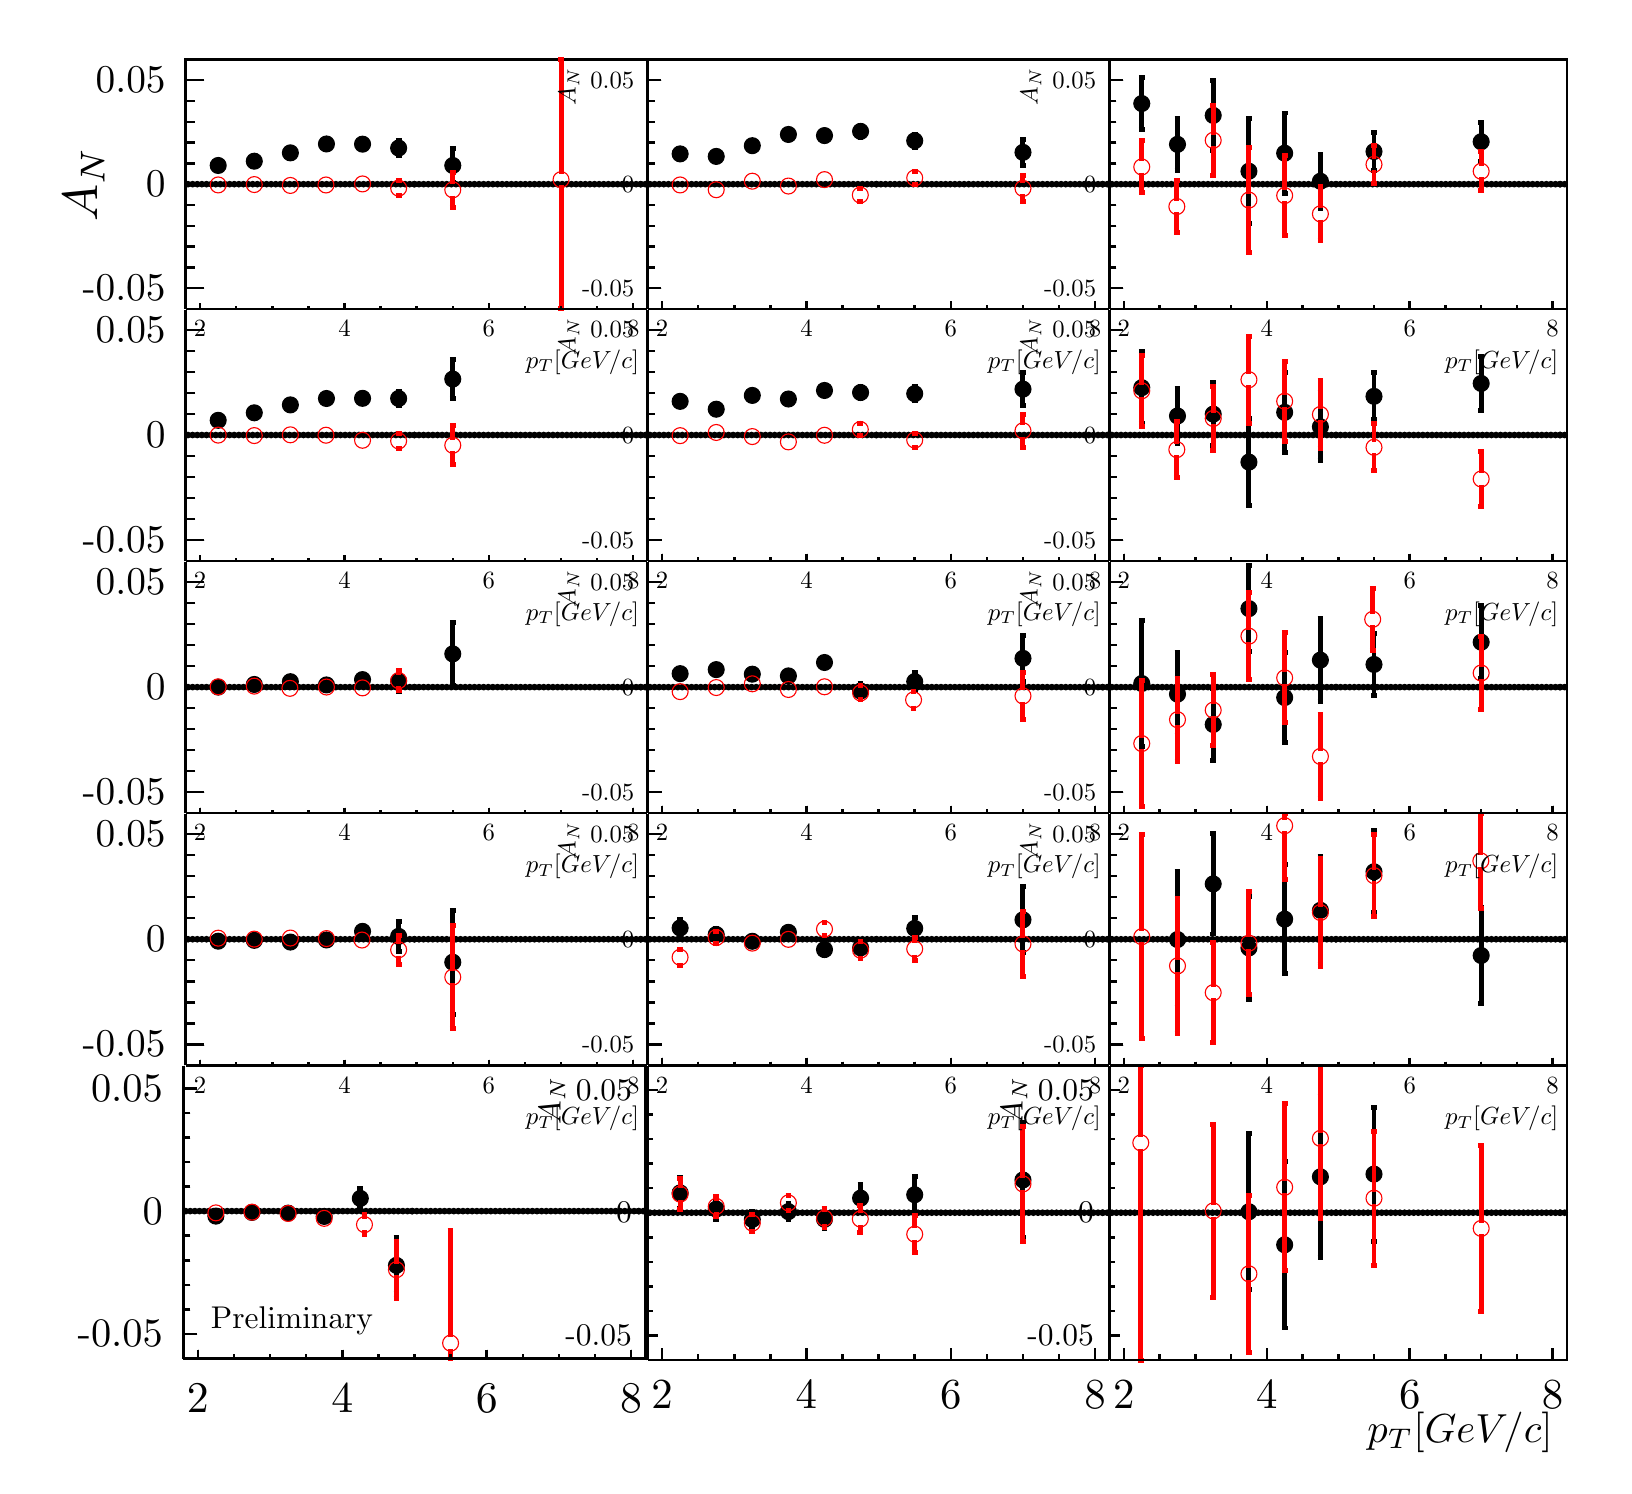
\begin{tikzpicture}
\pgfdeclareplotmark{cross} {
\pgfpathmoveto{\pgfpoint{-0.3\pgfplotmarksize}{\pgfplotmarksize}}
\pgfpathlineto{\pgfpoint{+0.3\pgfplotmarksize}{\pgfplotmarksize}}
\pgfpathlineto{\pgfpoint{+0.3\pgfplotmarksize}{0.3\pgfplotmarksize}}
\pgfpathlineto{\pgfpoint{+1\pgfplotmarksize}{0.3\pgfplotmarksize}}
\pgfpathlineto{\pgfpoint{+1\pgfplotmarksize}{-0.3\pgfplotmarksize}}
\pgfpathlineto{\pgfpoint{+0.3\pgfplotmarksize}{-0.3\pgfplotmarksize}}
\pgfpathlineto{\pgfpoint{+0.3\pgfplotmarksize}{-1.\pgfplotmarksize}}
\pgfpathlineto{\pgfpoint{-0.3\pgfplotmarksize}{-1.\pgfplotmarksize}}
\pgfpathlineto{\pgfpoint{-0.3\pgfplotmarksize}{-0.3\pgfplotmarksize}}
\pgfpathlineto{\pgfpoint{-1.\pgfplotmarksize}{-0.3\pgfplotmarksize}}
\pgfpathlineto{\pgfpoint{-1.\pgfplotmarksize}{0.3\pgfplotmarksize}}
\pgfpathlineto{\pgfpoint{-0.3\pgfplotmarksize}{0.3\pgfplotmarksize}}
\pgfpathclose
\pgfusepathqstroke
}
\pgfdeclareplotmark{cross*} {
\pgfpathmoveto{\pgfpoint{-0.3\pgfplotmarksize}{\pgfplotmarksize}}
\pgfpathlineto{\pgfpoint{+0.3\pgfplotmarksize}{\pgfplotmarksize}}
\pgfpathlineto{\pgfpoint{+0.3\pgfplotmarksize}{0.3\pgfplotmarksize}}
\pgfpathlineto{\pgfpoint{+1\pgfplotmarksize}{0.3\pgfplotmarksize}}
\pgfpathlineto{\pgfpoint{+1\pgfplotmarksize}{-0.3\pgfplotmarksize}}
\pgfpathlineto{\pgfpoint{+0.3\pgfplotmarksize}{-0.3\pgfplotmarksize}}
\pgfpathlineto{\pgfpoint{+0.3\pgfplotmarksize}{-1.\pgfplotmarksize}}
\pgfpathlineto{\pgfpoint{-0.3\pgfplotmarksize}{-1.\pgfplotmarksize}}
\pgfpathlineto{\pgfpoint{-0.3\pgfplotmarksize}{-0.3\pgfplotmarksize}}
\pgfpathlineto{\pgfpoint{-1.\pgfplotmarksize}{-0.3\pgfplotmarksize}}
\pgfpathlineto{\pgfpoint{-1.\pgfplotmarksize}{0.3\pgfplotmarksize}}
\pgfpathlineto{\pgfpoint{-0.3\pgfplotmarksize}{0.3\pgfplotmarksize}}
\pgfpathclose
\pgfusepathqfillstroke
}
\pgfdeclareplotmark{newstar} {
\pgfpathmoveto{\pgfqpoint{0pt}{\pgfplotmarksize}}
\pgfpathlineto{\pgfqpointpolar{44}{0.5\pgfplotmarksize}}
\pgfpathlineto{\pgfqpointpolar{18}{\pgfplotmarksize}}
\pgfpathlineto{\pgfqpointpolar{-20}{0.5\pgfplotmarksize}}
\pgfpathlineto{\pgfqpointpolar{-54}{\pgfplotmarksize}}
\pgfpathlineto{\pgfqpointpolar{-90}{0.5\pgfplotmarksize}}
\pgfpathlineto{\pgfqpointpolar{234}{\pgfplotmarksize}}
\pgfpathlineto{\pgfqpointpolar{198}{0.5\pgfplotmarksize}}
\pgfpathlineto{\pgfqpointpolar{162}{\pgfplotmarksize}}
\pgfpathlineto{\pgfqpointpolar{134}{0.5\pgfplotmarksize}}
\pgfpathclose
\pgfusepathqstroke
}
\pgfdeclareplotmark{newstar*} {
\pgfpathmoveto{\pgfqpoint{0pt}{\pgfplotmarksize}}
\pgfpathlineto{\pgfqpointpolar{44}{0.5\pgfplotmarksize}}
\pgfpathlineto{\pgfqpointpolar{18}{\pgfplotmarksize}}
\pgfpathlineto{\pgfqpointpolar{-20}{0.5\pgfplotmarksize}}
\pgfpathlineto{\pgfqpointpolar{-54}{\pgfplotmarksize}}
\pgfpathlineto{\pgfqpointpolar{-90}{0.5\pgfplotmarksize}}
\pgfpathlineto{\pgfqpointpolar{234}{\pgfplotmarksize}}
\pgfpathlineto{\pgfqpointpolar{198}{0.5\pgfplotmarksize}}
\pgfpathlineto{\pgfqpointpolar{162}{\pgfplotmarksize}}
\pgfpathlineto{\pgfqpointpolar{134}{0.5\pgfplotmarksize}}
\pgfpathclose
\pgfusepathqfillstroke
}
\definecolor{c}{rgb}{0.999,0.999,0.999};
\draw [color=c, fill=c] (0,0) rectangle (20,18.1918);
\definecolor{c}{rgb}{0,0,0};
\draw [anchor=base west] (0.2,0.181918) node[scale=1.01414, color=c, rotate=0]{Tue Oct  6 22:43:49 2020};
\definecolor{c}{rgb}{1,1,1};
\draw [color=c, fill=c] (0.039801,0.0365297) rectangle (7.9005,5.05936);
\draw [color=c, fill=c] (1.97015,1.2968) rectangle (7.8408,5.0411);
\definecolor{c}{rgb}{0,0,0};
\draw [c,line width=0.9] (1.97015,1.2968) -- (1.97015,5.0411) -- (7.8408,5.0411) -- (7.8408,1.2968) -- (1.97015,1.2968);
\definecolor{c}{rgb}{1,1,1};
\draw [color=c, fill=c] (1.97015,1.2968) rectangle (7.8408,5.0411);
\definecolor{c}{rgb}{0,0,0};
\draw [c,line width=0.9] (1.97015,1.2968) -- (1.97015,5.0411) -- (7.8408,5.0411) -- (7.8408,1.2968) -- (1.97015,1.2968);
\foreach \P in
 {(1.9995,3.16895),(2.05821,3.16895),(2.11692,3.16895),(2.17562,3.16895),(2.23433,3.16895),(2.29303,3.16895),(2.35174,3.16895),(2.41045,3.16895),(2.46915,3.16895),(2.52786,3.16895),(2.58657,3.16895),(2.64527,3.16895),(2.70398,3.16895),(2.76269,3.1689
5),(2.82139,3.16895),(2.8801,3.16895),(2.93881,3.16895),(2.99751,3.16895),(3.05622,3.16895),(3.11493,3.16895),(3.17363,3.16895),(3.23234,3.16895),(3.29104,3.16895),(3.34975,3.16895),(3.40846,3.16895),(3.46716,3.16895),(3.52587,3.16895),(3.58458,3.168
95),(3.64328,3.16895),(3.70199,3.16895),(3.7607,3.16895),(3.8194,3.16895),(3.87811,3.16895),(3.93682,3.16895),(3.99552,3.16895),(4.05423,3.16895),(4.11294,3.16895),(4.17164,3.16895),(4.23035,3.16895),(4.28905,3.16895),(4.34776,3.16895),(4.40647,3.168
95),(4.46517,3.16895),(4.52388,3.16895),(4.58259,3.16895),(4.64129,3.16895),(4.7,3.16895),(4.75871,3.16895),(4.81741,3.16895),(4.87612,3.16895)}{\draw[mark options={color=c,fill=c},mark size=2.402402pt,mark=*,mark size=1pt] plot coordinates {\P};}
\foreach \P in
 {(4.87612,3.16895),(4.93483,3.16895),(4.99353,3.16895),(5.05224,3.16895),(5.11095,3.16895),(5.16965,3.16895),(5.22836,3.16895),(5.28706,3.16895),(5.34577,3.16895),(5.40448,3.16895),(5.46318,3.16895),(5.52189,3.16895),(5.5806,3.16895),(5.6393,3.16895
),(5.69801,3.16895),(5.75672,3.16895),(5.81542,3.16895),(5.87413,3.16895),(5.93284,3.16895),(5.99154,3.16895),(6.05025,3.16895),(6.10896,3.16895),(6.16766,3.16895),(6.22637,3.16895),(6.28507,3.16895),(6.34378,3.16895),(6.40249,3.16895),(6.46119,3.168
95),(6.5199,3.16895),(6.57861,3.16895),(6.63731,3.16895),(6.69602,3.16895),(6.75473,3.16895),(6.81343,3.16895),(6.87214,3.16895),(6.93085,3.16895),(6.98955,3.16895),(7.04826,3.16895),(7.10697,3.16895),(7.16567,3.16895),(7.22438,3.16895),(7.28308,3.16
895),(7.34179,3.16895),(7.4005,3.16895),(7.4592,3.16895),(7.51791,3.16895),(7.57662,3.16895),(7.63532,3.16895),(7.69403,3.16895),(7.75274,3.16895)}{\draw[mark options={color=c,fill=c},mark size=2.402402pt,mark=*,mark size=1pt] plot coordinates {\P};}
\foreach \P in {(7.75274,3.16895),(7.81144,3.16895)}{\draw[mark options={color=c,fill=c},mark size=2.402402pt,mark=*,mark size=1pt] plot coordinates {\P};}
\draw [c,line width=0.9] (1.97015,1.2968) -- (7.8408,1.2968);
\draw [c,line width=0.9] (2.15361,1.40934) -- (2.15361,1.2968);
\draw [c,line width=0.9] (2.61225,1.35307) -- (2.61225,1.2968);
\draw [c,line width=0.9] (3.0709,1.35307) -- (3.0709,1.2968);
\draw [c,line width=0.9] (3.52954,1.35307) -- (3.52954,1.2968);
\draw [c,line width=0.9] (3.98818,1.40934) -- (3.98818,1.2968);
\draw [c,line width=0.9] (4.44683,1.35307) -- (4.44683,1.2968);
\draw [c,line width=0.9] (4.90547,1.35307) -- (4.90547,1.2968);
\draw [c,line width=0.9] (5.36412,1.35307) -- (5.36412,1.2968);
\draw [c,line width=0.9] (5.82276,1.40934) -- (5.82276,1.2968);
\draw [c,line width=0.9] (6.28141,1.35307) -- (6.28141,1.2968);
\draw [c,line width=0.9] (6.74005,1.35307) -- (6.74005,1.2968);
\draw [c,line width=0.9] (7.19869,1.35307) -- (7.19869,1.2968);
\draw [c,line width=0.9] (7.65734,1.40934) -- (7.65734,1.2968);
\draw [c,line width=0.9] (2.15361,1.40934) -- (2.15361,1.2968);
\draw [c,line width=0.9] (7.65734,1.40934) -- (7.65734,1.2968);
\draw [anchor=base] (2.15361,0.608676) node[scale=1.58206, color=c, rotate=0]{2};
\draw [anchor=base] (3.98818,0.608676) node[scale=1.58206, color=c, rotate=0]{4};
\draw [anchor=base] (5.82276,0.608676) node[scale=1.58206, color=c, rotate=0]{6};
\draw [anchor=base] (7.65734,0.608676) node[scale=1.58206, color=c, rotate=0]{8};
\draw [c,line width=0.9] (1.97015,1.2968) -- (1.97015,5.0411);
\draw [c,line width=0.9] (2.14594,1.60883) -- (1.97015,1.60883);
\draw [c,line width=0.9] (2.05805,1.92085) -- (1.97015,1.92085);
\draw [c,line width=0.9] (2.05805,2.23288) -- (1.97015,2.23288);
\draw [c,line width=0.9] (2.05805,2.5449) -- (1.97015,2.5449);
\draw [c,line width=0.9] (2.05805,2.85693) -- (1.97015,2.85693);
\draw [c,line width=0.9] (2.14594,3.16895) -- (1.97015,3.16895);
\draw [c,line width=0.9] (2.05805,3.48097) -- (1.97015,3.48097);
\draw [c,line width=0.9] (2.05805,3.793) -- (1.97015,3.793);
\draw [c,line width=0.9] (2.05805,4.10502) -- (1.97015,4.10502);
\draw [c,line width=0.9] (2.05805,4.41705) -- (1.97015,4.41705);
\draw [c,line width=0.9] (2.14594,4.72907) -- (1.97015,4.72907);
\draw [c,line width=0.9] (2.14594,1.60883) -- (1.97015,1.60883);
\draw [c,line width=0.9] (2.05805,1.2968) -- (1.97015,1.2968);
\draw [c,line width=0.9] (2.14594,4.72907) -- (1.97015,4.72907);
\draw [c,line width=0.9] (2.05805,5.0411) -- (1.97015,5.0411);
\draw [anchor= east] (1.89154,1.60883) node[scale=1.46036, color=c, rotate=0]{-0.05};
\draw [anchor= east] (1.89154,3.16895) node[scale=1.46036, color=c, rotate=0]{0};
\draw [anchor= east] (1.89154,4.72907) node[scale=1.46036, color=c, rotate=0]{0.05};
\draw [c,line width=1.8] (4.21751,3.40307) -- (4.21751,3.45855);
\draw [c,line width=1.8] (4.18098,3.45855) -- (4.25404,3.45855);
\draw [c,line width=1.8] (4.21751,3.25695) -- (4.21751,3.20147);
\draw [c,line width=1.8] (4.18098,3.20147) -- (4.25404,3.20147);
\draw [c,line width=1.8] (4.67615,2.55299) -- (4.67615,2.83957);
\draw [c,line width=1.8] (4.63962,2.83957) -- (4.71268,2.83957);
\draw [c,line width=1.8] (4.67615,2.40687) -- (4.67615,2.12029);
\draw [c,line width=1.8] (4.63962,2.12029) -- (4.71268,2.12029);
\foreach \P in {(2.38293,3.10566),(2.84157,3.15245),(3.30022,3.14349),(3.75886,3.10138),(4.21751,3.33001),(4.67615,2.47993)}{\draw[mark options={color=c,fill=c},mark size=2.882883pt,mark=*] plot coordinates {\P};}
\definecolor{c}{rgb}{1,0,0};
\draw [c,line width=1.8] (4.27022,3.07046) -- (4.27022,3.12595);
\draw [c,line width=1.8] (4.23369,3.12595) -- (4.30675,3.12595);
\draw [c,line width=1.8] (4.27022,2.92435) -- (4.27022,2.86886);
\draw [c,line width=1.8] (4.23369,2.86886) -- (4.30675,2.86886);
\draw [c,line width=1.8] (4.67615,2.49797) -- (4.67615,2.78459);
\draw [c,line width=1.8] (4.63962,2.78459) -- (4.71268,2.78459);
\draw [c,line width=1.8] (4.67615,2.35185) -- (4.67615,2.06524);
\draw [c,line width=1.8] (4.63962,2.06524) -- (4.71268,2.06524);
\draw [c,line width=1.8] (5.36412,1.56534) -- (5.36412,2.9186);
\draw [c,line width=1.8] (5.32759,2.9186) -- (5.40065,2.9186);
\draw [c,line width=1.8] (5.36412,1.41922) -- (5.36412,1.2968);
\draw [c,line width=1.8] (5.32759,1.2968) -- (5.40065,1.2968);
\foreach \P in {(2.38293,3.14675),(2.84157,3.15559),(3.30022,3.13938),(3.75886,3.07716),(4.27022,2.9974),(4.67615,2.42491),(5.36412,1.49228)}{\draw[mark options={color=c,fill=c},mark size=2.882883pt,mark=o] plot coordinates {\P};}
\definecolor{c}{rgb}{0,0,0};
\draw [anchor=base west] (2.17925,1.67905) node[scale=1.13584, color=c, rotate=0]{Preliminary};
\draw [c,line width=0.9] (1.97015,1.2968) -- (7.8408,1.2968);
\draw [c,line width=0.9] (2.15361,1.40934) -- (2.15361,1.2968);
\draw [c,line width=0.9] (2.61225,1.35307) -- (2.61225,1.2968);
\draw [c,line width=0.9] (3.0709,1.35307) -- (3.0709,1.2968);
\draw [c,line width=0.9] (3.52954,1.35307) -- (3.52954,1.2968);
\draw [c,line width=0.9] (3.98818,1.40934) -- (3.98818,1.2968);
\draw [c,line width=0.9] (4.44683,1.35307) -- (4.44683,1.2968);
\draw [c,line width=0.9] (4.90547,1.35307) -- (4.90547,1.2968);
\draw [c,line width=0.9] (5.36412,1.35307) -- (5.36412,1.2968);
\draw [c,line width=0.9] (5.82276,1.40934) -- (5.82276,1.2968);
\draw [c,line width=0.9] (6.28141,1.35307) -- (6.28141,1.2968);
\draw [c,line width=0.9] (6.74005,1.35307) -- (6.74005,1.2968);
\draw [c,line width=0.9] (7.19869,1.35307) -- (7.19869,1.2968);
\draw [c,line width=0.9] (7.65734,1.40934) -- (7.65734,1.2968);
\draw [c,line width=0.9] (2.15361,1.40934) -- (2.15361,1.2968);
\draw [c,line width=0.9] (7.65734,1.40934) -- (7.65734,1.2968);
\draw [c,line width=0.9] (1.97015,1.2968) -- (1.97015,5.0411);
\draw [c,line width=0.9] (2.14594,1.60883) -- (1.97015,1.60883);
\draw [c,line width=0.9] (2.05805,1.92085) -- (1.97015,1.92085);
\draw [c,line width=0.9] (2.05805,2.23288) -- (1.97015,2.23288);
\draw [c,line width=0.9] (2.05805,2.5449) -- (1.97015,2.5449);
\draw [c,line width=0.9] (2.05805,2.85693) -- (1.97015,2.85693);
\draw [c,line width=0.9] (2.14594,3.16895) -- (1.97015,3.16895);
\draw [c,line width=0.9] (2.05805,3.48097) -- (1.97015,3.48097);
\draw [c,line width=0.9] (2.05805,3.793) -- (1.97015,3.793);
\draw [c,line width=0.9] (2.05805,4.10502) -- (1.97015,4.10502);
\draw [c,line width=0.9] (2.05805,4.41705) -- (1.97015,4.41705);
\draw [c,line width=0.9] (2.14594,4.72907) -- (1.97015,4.72907);
\draw [c,line width=0.9] (2.14594,1.60883) -- (1.97015,1.60883);
\draw [c,line width=0.9] (2.05805,1.2968) -- (1.97015,1.2968);
\draw [c,line width=0.9] (2.14594,4.72907) -- (1.97015,4.72907);
\draw [c,line width=0.9] (2.05805,5.0411) -- (1.97015,5.0411);
\definecolor{c}{rgb}{1,1,1};
\draw [color=c, fill=c] (0,5.02093) rectangle (7.86667,8.22268);
\draw [color=c, fill=c] (2,5.02093) rectangle (7.86667,8.22268);
\definecolor{c}{rgb}{0,0,0};
\draw [c,line width=0.9] (2,5.02093) -- (2,8.22268) -- (7.86667,8.22268) -- (7.86667,5.02093) -- (2,5.02093);
\definecolor{c}{rgb}{1,1,1};
\draw [color=c, fill=c] (2,5.02093) rectangle (7.86667,8.22268);
\definecolor{c}{rgb}{0,0,0};
\draw [c,line width=0.9] (2,5.02093) -- (2,8.22268) -- (7.86667,8.22268) -- (7.86667,5.02093) -- (2,5.02093);
\foreach \P in
 {(2.02933,6.62181),(2.088,6.62181),(2.14667,6.62181),(2.20533,6.62181),(2.264,6.62181),(2.32267,6.62181),(2.38133,6.62181),(2.44,6.62181),(2.49867,6.62181),(2.55733,6.62181),(2.616,6.62181),(2.67467,6.62181),(2.73333,6.62181),(2.792,6.62181),(2.8506
7,6.62181),(2.90933,6.62181),(2.968,6.62181),(3.02667,6.62181),(3.08533,6.62181),(3.144,6.62181),(3.20267,6.62181),(3.26133,6.62181),(3.32,6.62181),(3.37867,6.62181),(3.43733,6.62181),(3.496,6.62181),(3.55467,6.62181),(3.61333,6.62181),(3.672,6.62181
),(3.73067,6.62181),(3.78933,6.62181),(3.848,6.62181),(3.90667,6.62181),(3.96533,6.62181),(4.024,6.62181),(4.08267,6.62181),(4.14133,6.62181),(4.2,6.62181),(4.25867,6.62181),(4.31733,6.62181),(4.376,6.62181),(4.43467,6.62181),(4.49333,6.62181),(4.552
,6.62181),(4.61067,6.62181),(4.66933,6.62181),(4.728,6.62181),(4.78667,6.62181),(4.84533,6.62181),(4.904,6.62181)}{\draw[mark options={color=c,fill=c},mark size=2.402402pt,mark=*,mark size=1pt] plot coordinates {\P};}
\foreach \P in
 {(4.904,6.62181),(4.96267,6.62181),(5.02133,6.62181),(5.08,6.62181),(5.13867,6.62181),(5.19733,6.62181),(5.256,6.62181),(5.31467,6.62181),(5.37333,6.62181),(5.432,6.62181),(5.49067,6.62181),(5.54933,6.62181),(5.608,6.62181),(5.66667,6.62181),(5.7253
3,6.62181),(5.784,6.62181),(5.84267,6.62181),(5.90133,6.62181),(5.96,6.62181),(6.01867,6.62181),(6.07733,6.62181),(6.136,6.62181),(6.19467,6.62181),(6.25333,6.62181),(6.312,6.62181),(6.37067,6.62181),(6.42933,6.62181),(6.488,6.62181),(6.54667,6.62181
),(6.60533,6.62181),(6.664,6.62181),(6.72267,6.62181),(6.78133,6.62181),(6.84,6.62181),(6.89867,6.62181),(6.95733,6.62181),(7.016,6.62181),(7.07467,6.62181),(7.13333,6.62181),(7.192,6.62181),(7.25067,6.62181),(7.30933,6.62181),(7.368,6.62181),(7.4266
7,6.62181),(7.48533,6.62181),(7.544,6.62181),(7.60267,6.62181),(7.66133,6.62181),(7.72,6.62181),(7.77867,6.62181)}{\draw[mark options={color=c,fill=c},mark size=2.402402pt,mark=*,mark size=1pt] plot coordinates {\P};}
\foreach \P in {(7.77867,6.62181),(7.83733,6.62181)}{\draw[mark options={color=c,fill=c},mark size=2.402402pt,mark=*,mark size=1pt] plot coordinates {\P};}
\draw [c,line width=0.9] (2,5.02093) -- (7.86667,5.02093);
\draw [anchor= east] (7.86667,4.34856) node[scale=0.893954, color=c, rotate=0]{$p_{T} [GeV/c]$};
\draw [c,line width=0.9] (2.18333,5.09256) -- (2.18333,5.02093);
\draw [c,line width=0.9] (2.64167,5.05675) -- (2.64167,5.02093);
\draw [c,line width=0.9] (3.1,5.05675) -- (3.1,5.02093);
\draw [c,line width=0.9] (3.55833,5.05675) -- (3.55833,5.02093);
\draw [c,line width=0.9] (4.01667,5.09256) -- (4.01667,5.02093);
\draw [c,line width=0.9] (4.475,5.05675) -- (4.475,5.02093);
\draw [c,line width=0.9] (4.93333,5.05675) -- (4.93333,5.02093);
\draw [c,line width=0.9] (5.39167,5.05675) -- (5.39167,5.02093);
\draw [c,line width=0.9] (5.85,5.09256) -- (5.85,5.02093);
\draw [c,line width=0.9] (6.30833,5.05675) -- (6.30833,5.02093);
\draw [c,line width=0.9] (6.76667,5.05675) -- (6.76667,5.02093);
\draw [c,line width=0.9] (7.225,5.05675) -- (7.225,5.02093);
\draw [c,line width=0.9] (7.68333,5.09256) -- (7.68333,5.02093);
\draw [c,line width=0.9] (2.18333,5.09256) -- (2.18333,5.02093);
\draw [c,line width=0.9] (7.68333,5.09256) -- (7.68333,5.02093);
\draw [anchor=base] (2.18333,4.66874) node[scale=0.893954, color=c, rotate=0]{2};
\draw [anchor=base] (4.01667,4.66874) node[scale=0.893954, color=c, rotate=0]{4};
\draw [anchor=base] (5.85,4.66874) node[scale=0.893954, color=c, rotate=0]{6};
\draw [anchor=base] (7.68333,4.66874) node[scale=0.893954, color=c, rotate=0]{8};
\draw [c,line width=0.9] (2,5.02093) -- (2,8.22268);
\draw [c,line width=0.9] (2.236,5.28774) -- (2,5.28774);
\draw [c,line width=0.9] (2.118,5.55456) -- (2,5.55456);
\draw [c,line width=0.9] (2.118,5.82137) -- (2,5.82137);
\draw [c,line width=0.9] (2.118,6.08818) -- (2,6.08818);
\draw [c,line width=0.9] (2.118,6.355) -- (2,6.355);
\draw [c,line width=0.9] (2.236,6.62181) -- (2,6.62181);
\draw [c,line width=0.9] (2.118,6.88862) -- (2,6.88862);
\draw [c,line width=0.9] (2.118,7.15543) -- (2,7.15543);
\draw [c,line width=0.9] (2.118,7.42225) -- (2,7.42225);
\draw [c,line width=0.9] (2.118,7.68906) -- (2,7.68906);
\draw [c,line width=0.9] (2.236,7.95587) -- (2,7.95587);
\draw [c,line width=0.9] (2.236,5.28774) -- (2,5.28774);
\draw [c,line width=0.9] (2.118,5.02093) -- (2,5.02093);
\draw [c,line width=0.9] (2.236,7.95587) -- (2,7.95587);
\draw [c,line width=0.9] (2.118,8.22268) -- (2,8.22268);
\draw [anchor= east] (1.92133,5.28774) node[scale=1.4222, color=c, rotate=0]{-0.05};
\draw [anchor= east] (1.92133,6.62181) node[scale=1.4222, color=c, rotate=0]{0};
\draw [anchor= east] (1.92133,7.95587) node[scale=1.4222, color=c, rotate=0]{0.05};
\draw [c,line width=1.8] (4.70417,6.73148) -- (4.70417,6.84463);
\draw [c,line width=1.8] (4.66764,6.84463) -- (4.7407,6.84463);
\draw [c,line width=1.8] (4.70417,6.58536) -- (4.70417,6.47221);
\draw [c,line width=1.8] (4.66764,6.47221) -- (4.7407,6.47221);
\draw [c,line width=1.8] (5.39167,6.40308) -- (5.39167,6.98861);
\draw [c,line width=1.8] (5.35514,6.98861) -- (5.4282,6.98861);
\draw [c,line width=1.8] (5.39167,6.25697) -- (5.39167,5.67144);
\draw [c,line width=1.8] (5.35514,5.67144) -- (5.4282,5.67144);
\foreach \P in {(2.4125,6.597),(2.87083,6.60782),(3.32917,6.58615),(3.7875,6.61266),(4.24583,6.72172),(4.70417,6.65842),(5.39167,6.33002)}{\draw[mark options={color=c,fill=c},mark size=2.882883pt,mark=*] plot coordinates {\P};}
\definecolor{c}{rgb}{1,0,0};
\draw [c,line width=1.8] (4.70417,6.56136) -- (4.70417,6.67448);
\draw [c,line width=1.8] (4.66764,6.67448) -- (4.7407,6.67448);
\draw [c,line width=1.8] (4.70417,6.41525) -- (4.70417,6.30213);
\draw [c,line width=1.8] (4.66764,6.30213) -- (4.7407,6.30213);
\draw [c,line width=1.8] (5.39167,6.21353) -- (5.39167,6.79728);
\draw [c,line width=1.8] (5.35514,6.79728) -- (5.4282,6.79728);
\draw [c,line width=1.8] (5.39167,6.06741) -- (5.39167,5.48365);
\draw [c,line width=1.8] (5.35514,5.48365) -- (5.4282,5.48365);
\foreach \P in {(2.4125,6.63539),(2.87083,6.62337),(3.32917,6.63701),(3.7875,6.63032),(4.23881,6.61187),(4.70417,6.4883),(5.39167,6.14047)}{\draw[mark options={color=c,fill=c},mark size=2.882883pt,mark=o] plot coordinates {\P};}
\definecolor{c}{rgb}{0,0,0};
\draw [c,line width=0.9] (2,5.02093) -- (7.86667,5.02093);
\draw [c,line width=0.9] (2.18333,5.09256) -- (2.18333,5.02093);
\draw [c,line width=0.9] (2.64167,5.05675) -- (2.64167,5.02093);
\draw [c,line width=0.9] (3.1,5.05675) -- (3.1,5.02093);
\draw [c,line width=0.9] (3.55833,5.05675) -- (3.55833,5.02093);
\draw [c,line width=0.9] (4.01667,5.09256) -- (4.01667,5.02093);
\draw [c,line width=0.9] (4.475,5.05675) -- (4.475,5.02093);
\draw [c,line width=0.9] (4.93333,5.05675) -- (4.93333,5.02093);
\draw [c,line width=0.9] (5.39167,5.05675) -- (5.39167,5.02093);
\draw [c,line width=0.9] (5.85,5.09256) -- (5.85,5.02093);
\draw [c,line width=0.9] (6.30833,5.05675) -- (6.30833,5.02093);
\draw [c,line width=0.9] (6.76667,5.05675) -- (6.76667,5.02093);
\draw [c,line width=0.9] (7.225,5.05675) -- (7.225,5.02093);
\draw [c,line width=0.9] (7.68333,5.09256) -- (7.68333,5.02093);
\draw [c,line width=0.9] (2.18333,5.09256) -- (2.18333,5.02093);
\draw [c,line width=0.9] (7.68333,5.09256) -- (7.68333,5.02093);
\draw [c,line width=0.9] (2,5.02093) -- (2,8.22268);
\draw [c,line width=0.9] (2.236,5.28774) -- (2,5.28774);
\draw [c,line width=0.9] (2.118,5.55456) -- (2,5.55456);
\draw [c,line width=0.9] (2.118,5.82137) -- (2,5.82137);
\draw [c,line width=0.9] (2.118,6.08818) -- (2,6.08818);
\draw [c,line width=0.9] (2.118,6.355) -- (2,6.355);
\draw [c,line width=0.9] (2.236,6.62181) -- (2,6.62181);
\draw [c,line width=0.9] (2.118,6.88862) -- (2,6.88862);
\draw [c,line width=0.9] (2.118,7.15543) -- (2,7.15543);
\draw [c,line width=0.9] (2.118,7.42225) -- (2,7.42225);
\draw [c,line width=0.9] (2.118,7.68906) -- (2,7.68906);
\draw [c,line width=0.9] (2.236,7.95587) -- (2,7.95587);
\draw [c,line width=0.9] (2.236,5.28774) -- (2,5.28774);
\draw [c,line width=0.9] (2.118,5.02093) -- (2,5.02093);
\draw [c,line width=0.9] (2.236,7.95587) -- (2,7.95587);
\draw [c,line width=0.9] (2.118,8.22268) -- (2,8.22268);
\definecolor{c}{rgb}{1,1,1};
\draw [color=c, fill=c] (0,8.22268) rectangle (7.86667,11.4244);
\draw [color=c, fill=c] (2,8.22268) rectangle (7.86667,11.4244);
\definecolor{c}{rgb}{0,0,0};
\draw [c,line width=0.9] (2,8.22268) -- (2,11.4244) -- (7.86667,11.4244) -- (7.86667,8.22268) -- (2,8.22268);
\definecolor{c}{rgb}{1,1,1};
\draw [color=c, fill=c] (2,8.22268) rectangle (7.86667,11.4244);
\definecolor{c}{rgb}{0,0,0};
\draw [c,line width=0.9] (2,8.22268) -- (2,11.4244) -- (7.86667,11.4244) -- (7.86667,8.22268) -- (2,8.22268);
\foreach \P in
 {(2.02933,9.82356),(2.088,9.82356),(2.14667,9.82356),(2.20533,9.82356),(2.264,9.82356),(2.32267,9.82356),(2.38133,9.82356),(2.44,9.82356),(2.49867,9.82356),(2.55733,9.82356),(2.616,9.82356),(2.67467,9.82356),(2.73333,9.82356),(2.792,9.82356),(2.8506
7,9.82356),(2.90933,9.82356),(2.968,9.82356),(3.02667,9.82356),(3.08533,9.82356),(3.144,9.82356),(3.20267,9.82356),(3.26133,9.82356),(3.32,9.82356),(3.37867,9.82356),(3.43733,9.82356),(3.496,9.82356),(3.55467,9.82356),(3.61333,9.82356),(3.672,9.82356
),(3.73067,9.82356),(3.78933,9.82356),(3.848,9.82356),(3.90667,9.82356),(3.96533,9.82356),(4.024,9.82356),(4.08267,9.82356),(4.14133,9.82356),(4.2,9.82356),(4.25867,9.82356),(4.31733,9.82356),(4.376,9.82356),(4.43467,9.82356),(4.49333,9.82356),(4.552
,9.82356),(4.61067,9.82356),(4.66933,9.82356),(4.728,9.82356),(4.78667,9.82356),(4.84533,9.82356),(4.904,9.82356)}{\draw[mark options={color=c,fill=c},mark size=2.402402pt,mark=*,mark size=1pt] plot coordinates {\P};}
\foreach \P in
 {(4.904,9.82356),(4.96267,9.82356),(5.02133,9.82356),(5.08,9.82356),(5.13867,9.82356),(5.19733,9.82356),(5.256,9.82356),(5.31467,9.82356),(5.37333,9.82356),(5.432,9.82356),(5.49067,9.82356),(5.54933,9.82356),(5.608,9.82356),(5.66667,9.82356),(5.7253
3,9.82356),(5.784,9.82356),(5.84267,9.82356),(5.90133,9.82356),(5.96,9.82356),(6.01867,9.82356),(6.07733,9.82356),(6.136,9.82356),(6.19467,9.82356),(6.25333,9.82356),(6.312,9.82356),(6.37067,9.82356),(6.42933,9.82356),(6.488,9.82356),(6.54667,9.82356
),(6.60533,9.82356),(6.664,9.82356),(6.72267,9.82356),(6.78133,9.82356),(6.84,9.82356),(6.89867,9.82356),(6.95733,9.82356),(7.016,9.82356),(7.07467,9.82356),(7.13333,9.82356),(7.192,9.82356),(7.25067,9.82356),(7.30933,9.82356),(7.368,9.82356),(7.4266
7,9.82356),(7.48533,9.82356),(7.544,9.82356),(7.60267,9.82356),(7.66133,9.82356),(7.72,9.82356),(7.77867,9.82356)}{\draw[mark options={color=c,fill=c},mark size=2.402402pt,mark=*,mark size=1pt] plot coordinates {\P};}
\foreach \P in {(7.77867,9.82356),(7.83733,9.82356)}{\draw[mark options={color=c,fill=c},mark size=2.402402pt,mark=*,mark size=1pt] plot coordinates {\P};}
\draw [c,line width=0.9] (2,8.22268) -- (7.86667,8.22268);
\draw [anchor= east] (7.86667,7.55032) node[scale=0.893954, color=c, rotate=0]{$p_{T} [GeV/c]$};
\draw [c,line width=0.9] (2.18333,8.29432) -- (2.18333,8.22268);
\draw [c,line width=0.9] (2.64167,8.2585) -- (2.64167,8.22268);
\draw [c,line width=0.9] (3.1,8.2585) -- (3.1,8.22268);
\draw [c,line width=0.9] (3.55833,8.2585) -- (3.55833,8.22268);
\draw [c,line width=0.9] (4.01667,8.29432) -- (4.01667,8.22268);
\draw [c,line width=0.9] (4.475,8.2585) -- (4.475,8.22268);
\draw [c,line width=0.9] (4.93333,8.2585) -- (4.93333,8.22268);
\draw [c,line width=0.9] (5.39167,8.2585) -- (5.39167,8.22268);
\draw [c,line width=0.9] (5.85,8.29432) -- (5.85,8.22268);
\draw [c,line width=0.9] (6.30833,8.2585) -- (6.30833,8.22268);
\draw [c,line width=0.9] (6.76667,8.2585) -- (6.76667,8.22268);
\draw [c,line width=0.9] (7.225,8.2585) -- (7.225,8.22268);
\draw [c,line width=0.9] (7.68333,8.29432) -- (7.68333,8.22268);
\draw [c,line width=0.9] (2.18333,8.29432) -- (2.18333,8.22268);
\draw [c,line width=0.9] (7.68333,8.29432) -- (7.68333,8.22268);
\draw [anchor=base] (2.18333,7.87049) node[scale=0.893954, color=c, rotate=0]{2};
\draw [anchor=base] (4.01667,7.87049) node[scale=0.893954, color=c, rotate=0]{4};
\draw [anchor=base] (5.85,7.87049) node[scale=0.893954, color=c, rotate=0]{6};
\draw [anchor=base] (7.68333,7.87049) node[scale=0.893954, color=c, rotate=0]{8};
\draw [c,line width=0.9] (2,8.22268) -- (2,11.4244);
\draw [c,line width=0.9] (2.236,8.4895) -- (2,8.4895);
\draw [c,line width=0.9] (2.118,8.75631) -- (2,8.75631);
\draw [c,line width=0.9] (2.118,9.02312) -- (2,9.02312);
\draw [c,line width=0.9] (2.118,9.28994) -- (2,9.28994);
\draw [c,line width=0.9] (2.118,9.55675) -- (2,9.55675);
\draw [c,line width=0.9] (2.236,9.82356) -- (2,9.82356);
\draw [c,line width=0.9] (2.118,10.0904) -- (2,10.0904);
\draw [c,line width=0.9] (2.118,10.3572) -- (2,10.3572);
\draw [c,line width=0.9] (2.118,10.624) -- (2,10.624);
\draw [c,line width=0.9] (2.118,10.8908) -- (2,10.8908);
\draw [c,line width=0.9] (2.236,11.1576) -- (2,11.1576);
\draw [c,line width=0.9] (2.236,8.4895) -- (2,8.4895);
\draw [c,line width=0.9] (2.118,8.22268) -- (2,8.22268);
\draw [c,line width=0.9] (2.236,11.1576) -- (2,11.1576);
\draw [c,line width=0.9] (2.118,11.4244) -- (2,11.4244);
\draw [anchor= east] (1.92133,8.4895) node[scale=1.4222, color=c, rotate=0]{-0.05};
\draw [anchor= east] (1.92133,9.82356) node[scale=1.4222, color=c, rotate=0]{0};
\draw [anchor= east] (1.92133,11.1576) node[scale=1.4222, color=c, rotate=0]{0.05};
\draw [c,line width=1.8] (4.70417,9.97171) -- (4.70417,10.0274);
\draw [c,line width=1.8] (4.66764,10.0274) -- (4.7407,10.0274);
\draw [c,line width=1.8] (4.70417,9.8256) -- (4.70417,9.76992);
\draw [c,line width=1.8] (4.66764,9.76992) -- (4.7407,9.76992);
\draw [c,line width=1.8] (5.39167,10.319) -- (5.39167,10.6432);
\draw [c,line width=1.8] (5.35514,10.6432) -- (5.4282,10.6432);
\draw [c,line width=1.8] (5.39167,10.1729) -- (5.39167,9.84873);
\draw [c,line width=1.8] (5.35514,9.84873) -- (5.4282,9.84873);
\foreach \P in {(2.4125,9.8241),(2.87083,9.85736),(3.32917,9.89271),(3.7875,9.85133),(4.24583,9.91905),(4.70417,9.89866),(5.39167,10.246)}{\draw[mark options={color=c,fill=c},mark size=2.882883pt,mark=*] plot coordinates {\P};}
\definecolor{c}{rgb}{1,0,0};
\draw [c,line width=1.8] (4.70417,9.97984) -- (4.70417,10.0355);
\draw [c,line width=1.8] (4.66764,10.0355) -- (4.7407,10.0355);
\draw [c,line width=1.8] (4.70417,9.83372) -- (4.70417,9.77805);
\draw [c,line width=1.8] (4.66764,9.77805) -- (4.7407,9.77805);
\foreach \P in {(2.4125,9.82723),(2.87083,9.83619),(3.32338,9.80822),(3.7875,9.82486),(4.24583,9.81414),(4.70417,9.90678)}{\draw[mark options={color=c,fill=c},mark size=2.882883pt,mark=o] plot coordinates {\P};}
\definecolor{c}{rgb}{0,0,0};
\draw [c,line width=0.9] (2,8.22268) -- (7.86667,8.22268);
\draw [c,line width=0.9] (2.18333,8.29432) -- (2.18333,8.22268);
\draw [c,line width=0.9] (2.64167,8.2585) -- (2.64167,8.22268);
\draw [c,line width=0.9] (3.1,8.2585) -- (3.1,8.22268);
\draw [c,line width=0.9] (3.55833,8.2585) -- (3.55833,8.22268);
\draw [c,line width=0.9] (4.01667,8.29432) -- (4.01667,8.22268);
\draw [c,line width=0.9] (4.475,8.2585) -- (4.475,8.22268);
\draw [c,line width=0.9] (4.93333,8.2585) -- (4.93333,8.22268);
\draw [c,line width=0.9] (5.39167,8.2585) -- (5.39167,8.22268);
\draw [c,line width=0.9] (5.85,8.29432) -- (5.85,8.22268);
\draw [c,line width=0.9] (6.30833,8.2585) -- (6.30833,8.22268);
\draw [c,line width=0.9] (6.76667,8.2585) -- (6.76667,8.22268);
\draw [c,line width=0.9] (7.225,8.2585) -- (7.225,8.22268);
\draw [c,line width=0.9] (7.68333,8.29432) -- (7.68333,8.22268);
\draw [c,line width=0.9] (2.18333,8.29432) -- (2.18333,8.22268);
\draw [c,line width=0.9] (7.68333,8.29432) -- (7.68333,8.22268);
\draw [c,line width=0.9] (2,8.22268) -- (2,11.4244);
\draw [c,line width=0.9] (2.236,8.4895) -- (2,8.4895);
\draw [c,line width=0.9] (2.118,8.75631) -- (2,8.75631);
\draw [c,line width=0.9] (2.118,9.02312) -- (2,9.02312);
\draw [c,line width=0.9] (2.118,9.28994) -- (2,9.28994);
\draw [c,line width=0.9] (2.118,9.55675) -- (2,9.55675);
\draw [c,line width=0.9] (2.236,9.82356) -- (2,9.82356);
\draw [c,line width=0.9] (2.118,10.0904) -- (2,10.0904);
\draw [c,line width=0.9] (2.118,10.3572) -- (2,10.3572);
\draw [c,line width=0.9] (2.118,10.624) -- (2,10.624);
\draw [c,line width=0.9] (2.118,10.8908) -- (2,10.8908);
\draw [c,line width=0.9] (2.236,11.1576) -- (2,11.1576);
\draw [c,line width=0.9] (2.236,8.4895) -- (2,8.4895);
\draw [c,line width=0.9] (2.118,8.22268) -- (2,8.22268);
\draw [c,line width=0.9] (2.236,11.1576) -- (2,11.1576);
\draw [c,line width=0.9] (2.118,11.4244) -- (2,11.4244);
\definecolor{c}{rgb}{1,1,1};
\draw [color=c, fill=c] (0,11.4244) rectangle (7.86667,14.6262);
\draw [color=c, fill=c] (2,11.4244) rectangle (7.86667,14.6262);
\definecolor{c}{rgb}{0,0,0};
\draw [c,line width=0.9] (2,11.4244) -- (2,14.6262) -- (7.86667,14.6262) -- (7.86667,11.4244) -- (2,11.4244);
\definecolor{c}{rgb}{1,1,1};
\draw [color=c, fill=c] (2,11.4244) rectangle (7.86667,14.6262);
\definecolor{c}{rgb}{0,0,0};
\draw [c,line width=0.9] (2,11.4244) -- (2,14.6262) -- (7.86667,14.6262) -- (7.86667,11.4244) -- (2,11.4244);
\foreach \P in
 {(2.02933,13.0253),(2.088,13.0253),(2.14667,13.0253),(2.20533,13.0253),(2.264,13.0253),(2.32267,13.0253),(2.38133,13.0253),(2.44,13.0253),(2.49867,13.0253),(2.55733,13.0253),(2.616,13.0253),(2.67467,13.0253),(2.73333,13.0253),(2.792,13.0253),(2.8506
7,13.0253),(2.90933,13.0253),(2.968,13.0253),(3.02667,13.0253),(3.08533,13.0253),(3.144,13.0253),(3.20267,13.0253),(3.26133,13.0253),(3.32,13.0253),(3.37867,13.0253),(3.43733,13.0253),(3.496,13.0253),(3.55467,13.0253),(3.61333,13.0253),(3.672,13.0253
),(3.73067,13.0253),(3.78933,13.0253),(3.848,13.0253),(3.90667,13.0253),(3.96533,13.0253),(4.024,13.0253),(4.08267,13.0253),(4.14133,13.0253),(4.2,13.0253),(4.25867,13.0253),(4.31733,13.0253),(4.376,13.0253),(4.43467,13.0253),(4.49333,13.0253),(4.552
,13.0253),(4.61067,13.0253),(4.66933,13.0253),(4.728,13.0253),(4.78667,13.0253),(4.84533,13.0253),(4.904,13.0253)}{\draw[mark options={color=c,fill=c},mark size=2.402402pt,mark=*,mark size=1pt] plot coordinates {\P};}
\foreach \P in
 {(4.904,13.0253),(4.96267,13.0253),(5.02133,13.0253),(5.08,13.0253),(5.13867,13.0253),(5.19733,13.0253),(5.256,13.0253),(5.31467,13.0253),(5.37333,13.0253),(5.432,13.0253),(5.49067,13.0253),(5.54933,13.0253),(5.608,13.0253),(5.66667,13.0253),(5.7253
3,13.0253),(5.784,13.0253),(5.84267,13.0253),(5.90133,13.0253),(5.96,13.0253),(6.01867,13.0253),(6.07733,13.0253),(6.136,13.0253),(6.19467,13.0253),(6.25333,13.0253),(6.312,13.0253),(6.37067,13.0253),(6.42933,13.0253),(6.488,13.0253),(6.54667,13.0253
),(6.60533,13.0253),(6.664,13.0253),(6.72267,13.0253),(6.78133,13.0253),(6.84,13.0253),(6.89867,13.0253),(6.95733,13.0253),(7.016,13.0253),(7.07467,13.0253),(7.13333,13.0253),(7.192,13.0253),(7.25067,13.0253),(7.30933,13.0253),(7.368,13.0253),(7.4266
7,13.0253),(7.48533,13.0253),(7.544,13.0253),(7.60267,13.0253),(7.66133,13.0253),(7.72,13.0253),(7.77867,13.0253)}{\draw[mark options={color=c,fill=c},mark size=2.402402pt,mark=*,mark size=1pt] plot coordinates {\P};}
\foreach \P in {(7.77867,13.0253),(7.83733,13.0253)}{\draw[mark options={color=c,fill=c},mark size=2.402402pt,mark=*,mark size=1pt] plot coordinates {\P};}
\draw [c,line width=0.9] (2,11.4244) -- (7.86667,11.4244);
\draw [anchor= east] (7.86667,10.7521) node[scale=0.893954, color=c, rotate=0]{$p_{T} [GeV/c]$};
\draw [c,line width=0.9] (2.18333,11.4961) -- (2.18333,11.4244);
\draw [c,line width=0.9] (2.64167,11.4603) -- (2.64167,11.4244);
\draw [c,line width=0.9] (3.1,11.4603) -- (3.1,11.4244);
\draw [c,line width=0.9] (3.55833,11.4603) -- (3.55833,11.4244);
\draw [c,line width=0.9] (4.01667,11.4961) -- (4.01667,11.4244);
\draw [c,line width=0.9] (4.475,11.4603) -- (4.475,11.4244);
\draw [c,line width=0.9] (4.93333,11.4603) -- (4.93333,11.4244);
\draw [c,line width=0.9] (5.39167,11.4603) -- (5.39167,11.4244);
\draw [c,line width=0.9] (5.85,11.4961) -- (5.85,11.4244);
\draw [c,line width=0.9] (6.30833,11.4603) -- (6.30833,11.4244);
\draw [c,line width=0.9] (6.76667,11.4603) -- (6.76667,11.4244);
\draw [c,line width=0.9] (7.225,11.4603) -- (7.225,11.4244);
\draw [c,line width=0.9] (7.68333,11.4961) -- (7.68333,11.4244);
\draw [c,line width=0.9] (2.18333,11.4961) -- (2.18333,11.4244);
\draw [c,line width=0.9] (7.68333,11.4961) -- (7.68333,11.4244);
\draw [anchor=base] (2.18333,11.0722) node[scale=0.893954, color=c, rotate=0]{2};
\draw [anchor=base] (4.01667,11.0722) node[scale=0.893954, color=c, rotate=0]{4};
\draw [anchor=base] (5.85,11.0722) node[scale=0.893954, color=c, rotate=0]{6};
\draw [anchor=base] (7.68333,11.0722) node[scale=0.893954, color=c, rotate=0]{8};
\draw [c,line width=0.9] (2,11.4244) -- (2,14.6262);
\draw [c,line width=0.9] (2.236,11.6913) -- (2,11.6913);
\draw [c,line width=0.9] (2.118,11.9581) -- (2,11.9581);
\draw [c,line width=0.9] (2.118,12.2249) -- (2,12.2249);
\draw [c,line width=0.9] (2.118,12.4917) -- (2,12.4917);
\draw [c,line width=0.9] (2.118,12.7585) -- (2,12.7585);
\draw [c,line width=0.9] (2.236,13.0253) -- (2,13.0253);
\draw [c,line width=0.9] (2.118,13.2921) -- (2,13.2921);
\draw [c,line width=0.9] (2.118,13.5589) -- (2,13.5589);
\draw [c,line width=0.9] (2.118,13.8258) -- (2,13.8258);
\draw [c,line width=0.9] (2.118,14.0926) -- (2,14.0926);
\draw [c,line width=0.9] (2.236,14.3594) -- (2,14.3594);
\draw [c,line width=0.9] (2.236,11.6913) -- (2,11.6913);
\draw [c,line width=0.9] (2.118,11.4244) -- (2,11.4244);
\draw [c,line width=0.9] (2.236,14.3594) -- (2,14.3594);
\draw [c,line width=0.9] (2.118,14.6262) -- (2,14.6262);
\draw [anchor= east] (1.92133,11.6913) node[scale=1.4222, color=c, rotate=0]{-0.05};
\draw [anchor= east] (1.92133,13.0253) node[scale=1.4222, color=c, rotate=0]{0};
\draw [anchor= east] (1.92133,14.3594) node[scale=1.4222, color=c, rotate=0]{0.05};
\draw [c,line width=1.8] (4.70417,13.5624) -- (4.70417,13.5812);
\draw [c,line width=1.8] (4.66764,13.5812) -- (4.7407,13.5812);
\draw [c,line width=1.8] (4.70417,13.4163) -- (4.70417,13.3975);
\draw [c,line width=1.8] (4.66764,13.3975) -- (4.7407,13.3975);
\draw [c,line width=1.8] (5.39167,13.809) -- (5.39167,13.9833);
\draw [c,line width=1.8] (5.35514,13.9833) -- (5.4282,13.9833);
\draw [c,line width=1.8] (5.39167,13.6629) -- (5.39167,13.4885);
\draw [c,line width=1.8] (5.35514,13.4885) -- (5.4282,13.4885);
\foreach \P in {(2.4125,13.212),(2.87083,13.3075),(3.32917,13.408),(3.7875,13.4892),(4.24583,13.4911),(4.70417,13.4894),(5.39167,13.7359)}{\draw[mark options={color=c,fill=c},mark size=2.882883pt,mark=*] plot coordinates {\P};}
\definecolor{c}{rgb}{1,0,0};
\draw [c,line width=1.8] (4.70417,13.0235) -- (4.70417,13.0422);
\draw [c,line width=1.8] (4.66764,13.0422) -- (4.7407,13.0422);
\draw [c,line width=1.8] (4.70417,12.8774) -- (4.70417,12.8586);
\draw [c,line width=1.8] (4.66764,12.8586) -- (4.7407,12.8586);
\draw [c,line width=1.8] (5.39167,12.9682) -- (5.39167,13.1426);
\draw [c,line width=1.8] (5.35514,13.1426) -- (5.4282,13.1426);
\draw [c,line width=1.8] (5.39167,12.8221) -- (5.39167,12.6478);
\draw [c,line width=1.8] (5.35514,12.6478) -- (5.4282,12.6478);
\foreach \P in {(2.4125,13.0242),(2.87083,13.0183),(3.32917,13.0278),(3.78109,13.0228),(4.24583,12.9586),(4.70417,12.9504),(5.39167,12.8952)}{\draw[mark options={color=c,fill=c},mark size=2.882883pt,mark=o] plot coordinates {\P};}
\definecolor{c}{rgb}{0,0,0};
\draw [c,line width=0.9] (2,11.4244) -- (7.86667,11.4244);
\draw [c,line width=0.9] (2.18333,11.4961) -- (2.18333,11.4244);
\draw [c,line width=0.9] (2.64167,11.4603) -- (2.64167,11.4244);
\draw [c,line width=0.9] (3.1,11.4603) -- (3.1,11.4244);
\draw [c,line width=0.9] (3.55833,11.4603) -- (3.55833,11.4244);
\draw [c,line width=0.9] (4.01667,11.4961) -- (4.01667,11.4244);
\draw [c,line width=0.9] (4.475,11.4603) -- (4.475,11.4244);
\draw [c,line width=0.9] (4.93333,11.4603) -- (4.93333,11.4244);
\draw [c,line width=0.9] (5.39167,11.4603) -- (5.39167,11.4244);
\draw [c,line width=0.9] (5.85,11.4961) -- (5.85,11.4244);
\draw [c,line width=0.9] (6.30833,11.4603) -- (6.30833,11.4244);
\draw [c,line width=0.9] (6.76667,11.4603) -- (6.76667,11.4244);
\draw [c,line width=0.9] (7.225,11.4603) -- (7.225,11.4244);
\draw [c,line width=0.9] (7.68333,11.4961) -- (7.68333,11.4244);
\draw [c,line width=0.9] (2.18333,11.4961) -- (2.18333,11.4244);
\draw [c,line width=0.9] (7.68333,11.4961) -- (7.68333,11.4244);
\draw [c,line width=0.9] (2,11.4244) -- (2,14.6262);
\draw [c,line width=0.9] (2.236,11.6913) -- (2,11.6913);
\draw [c,line width=0.9] (2.118,11.9581) -- (2,11.9581);
\draw [c,line width=0.9] (2.118,12.2249) -- (2,12.2249);
\draw [c,line width=0.9] (2.118,12.4917) -- (2,12.4917);
\draw [c,line width=0.9] (2.118,12.7585) -- (2,12.7585);
\draw [c,line width=0.9] (2.236,13.0253) -- (2,13.0253);
\draw [c,line width=0.9] (2.118,13.2921) -- (2,13.2921);
\draw [c,line width=0.9] (2.118,13.5589) -- (2,13.5589);
\draw [c,line width=0.9] (2.118,13.8258) -- (2,13.8258);
\draw [c,line width=0.9] (2.118,14.0926) -- (2,14.0926);
\draw [c,line width=0.9] (2.236,14.3594) -- (2,14.3594);
\draw [c,line width=0.9] (2.236,11.6913) -- (2,11.6913);
\draw [c,line width=0.9] (2.118,11.4244) -- (2,11.4244);
\draw [c,line width=0.9] (2.236,14.3594) -- (2,14.3594);
\draw [c,line width=0.9] (2.118,14.6262) -- (2,14.6262);
\definecolor{c}{rgb}{1,1,1};
\draw [color=c, fill=c] (0,14.6262) rectangle (7.86667,17.8279);
\draw [color=c, fill=c] (2,14.6262) rectangle (7.86667,17.7959);
\definecolor{c}{rgb}{0,0,0};
\draw [c,line width=0.9] (2,14.6262) -- (2,17.7959) -- (7.86667,17.7959) -- (7.86667,14.6262) -- (2,14.6262);
\definecolor{c}{rgb}{1,1,1};
\draw [color=c, fill=c] (2,14.6262) rectangle (7.86667,17.7959);
\definecolor{c}{rgb}{0,0,0};
\draw [c,line width=0.9] (2,14.6262) -- (2,17.7959) -- (7.86667,17.7959) -- (7.86667,14.6262) -- (2,14.6262);
\foreach \P in
 {(2.02933,16.2111),(2.088,16.2111),(2.14667,16.2111),(2.20533,16.2111),(2.264,16.2111),(2.32267,16.2111),(2.38133,16.2111),(2.44,16.2111),(2.49867,16.2111),(2.55733,16.2111),(2.616,16.2111),(2.67467,16.2111),(2.73333,16.2111),(2.792,16.2111),(2.8506
7,16.2111),(2.90933,16.2111),(2.968,16.2111),(3.02667,16.2111),(3.08533,16.2111),(3.144,16.2111),(3.20267,16.2111),(3.26133,16.2111),(3.32,16.2111),(3.37867,16.2111),(3.43733,16.2111),(3.496,16.2111),(3.55467,16.2111),(3.61333,16.2111),(3.672,16.2111
),(3.73067,16.2111),(3.78933,16.2111),(3.848,16.2111),(3.90667,16.2111),(3.96533,16.2111),(4.024,16.2111),(4.08267,16.2111),(4.14133,16.2111),(4.2,16.2111),(4.25867,16.2111),(4.31733,16.2111),(4.376,16.2111),(4.43467,16.2111),(4.49333,16.2111),(4.552
,16.2111),(4.61067,16.2111),(4.66933,16.2111),(4.728,16.2111),(4.78667,16.2111),(4.84533,16.2111),(4.904,16.2111)}{\draw[mark options={color=c,fill=c},mark size=2.402402pt,mark=*,mark size=1pt] plot coordinates {\P};}
\foreach \P in
 {(4.904,16.2111),(4.96267,16.2111),(5.02133,16.2111),(5.08,16.2111),(5.13867,16.2111),(5.19733,16.2111),(5.256,16.2111),(5.31467,16.2111),(5.37333,16.2111),(5.432,16.2111),(5.49067,16.2111),(5.54933,16.2111),(5.608,16.2111),(5.66667,16.2111),(5.7253
3,16.2111),(5.784,16.2111),(5.84267,16.2111),(5.90133,16.2111),(5.96,16.2111),(6.01867,16.2111),(6.07733,16.2111),(6.136,16.2111),(6.19467,16.2111),(6.25333,16.2111),(6.312,16.2111),(6.37067,16.2111),(6.42933,16.2111),(6.488,16.2111),(6.54667,16.2111
),(6.60533,16.2111),(6.664,16.2111),(6.72267,16.2111),(6.78133,16.2111),(6.84,16.2111),(6.89867,16.2111),(6.95733,16.2111),(7.016,16.2111),(7.07467,16.2111),(7.13333,16.2111),(7.192,16.2111),(7.25067,16.2111),(7.30933,16.2111),(7.368,16.2111),(7.4266
7,16.2111),(7.48533,16.2111),(7.544,16.2111),(7.60267,16.2111),(7.66133,16.2111),(7.72,16.2111),(7.77867,16.2111)}{\draw[mark options={color=c,fill=c},mark size=2.402402pt,mark=*,mark size=1pt] plot coordinates {\P};}
\foreach \P in {(7.77867,16.2111),(7.83733,16.2111)}{\draw[mark options={color=c,fill=c},mark size=2.402402pt,mark=*,mark size=1pt] plot coordinates {\P};}
\draw [c,line width=0.9] (2,14.6262) -- (7.86667,14.6262);
\draw [anchor= east] (7.86667,13.9538) node[scale=0.893954, color=c, rotate=0]{$p_{T} [GeV/c]$};
\draw [c,line width=0.9] (2.18333,14.6978) -- (2.18333,14.6262);
\draw [c,line width=0.9] (2.64167,14.662) -- (2.64167,14.6262);
\draw [c,line width=0.9] (3.1,14.662) -- (3.1,14.6262);
\draw [c,line width=0.9] (3.55833,14.662) -- (3.55833,14.6262);
\draw [c,line width=0.9] (4.01667,14.6978) -- (4.01667,14.6262);
\draw [c,line width=0.9] (4.475,14.662) -- (4.475,14.6262);
\draw [c,line width=0.9] (4.93333,14.662) -- (4.93333,14.6262);
\draw [c,line width=0.9] (5.39167,14.662) -- (5.39167,14.6262);
\draw [c,line width=0.9] (5.85,14.6978) -- (5.85,14.6262);
\draw [c,line width=0.9] (6.30833,14.662) -- (6.30833,14.6262);
\draw [c,line width=0.9] (6.76667,14.662) -- (6.76667,14.6262);
\draw [c,line width=0.9] (7.225,14.662) -- (7.225,14.6262);
\draw [c,line width=0.9] (7.68333,14.6978) -- (7.68333,14.6262);
\draw [c,line width=0.9] (2.18333,14.6978) -- (2.18333,14.6262);
\draw [c,line width=0.9] (7.68333,14.6978) -- (7.68333,14.6262);
\draw [anchor=base] (2.18333,14.274) node[scale=0.893954, color=c, rotate=0]{2};
\draw [anchor=base] (4.01667,14.274) node[scale=0.893954, color=c, rotate=0]{4};
\draw [anchor=base] (5.85,14.274) node[scale=0.893954, color=c, rotate=0]{6};
\draw [anchor=base] (7.68333,14.274) node[scale=0.893954, color=c, rotate=0]{8};
\draw [c,line width=0.9] (2,14.6262) -- (2,17.7959);
\draw (0.709867,16.2111) node[scale=1.78791, color=c, rotate=90]{$A_{N}$};
\draw [c,line width=0.9] (2.23364,14.8903) -- (2,14.8903);
\draw [c,line width=0.9] (2.11682,15.1545) -- (2,15.1545);
\draw [c,line width=0.9] (2.11682,15.4186) -- (2,15.4186);
\draw [c,line width=0.9] (2.11682,15.6828) -- (2,15.6828);
\draw [c,line width=0.9] (2.11682,15.9469) -- (2,15.9469);
\draw [c,line width=0.9] (2.23364,16.2111) -- (2,16.2111);
\draw [c,line width=0.9] (2.11682,16.4752) -- (2,16.4752);
\draw [c,line width=0.9] (2.11682,16.7393) -- (2,16.7393);
\draw [c,line width=0.9] (2.11682,17.0035) -- (2,17.0035);
\draw [c,line width=0.9] (2.11682,17.2676) -- (2,17.2676);
\draw [c,line width=0.9] (2.23364,17.5318) -- (2,17.5318);
\draw [c,line width=0.9] (2.23364,14.8903) -- (2,14.8903);
\draw [c,line width=0.9] (2.11682,14.6262) -- (2,14.6262);
\draw [c,line width=0.9] (2.23364,17.5318) -- (2,17.5318);
\draw [c,line width=0.9] (2.11682,17.7959) -- (2,17.7959);
\draw [anchor= east] (1.92133,14.8903) node[scale=1.4222, color=c, rotate=0]{-0.05};
\draw [anchor= east] (1.92133,16.2111) node[scale=1.4222, color=c, rotate=0]{0};
\draw [anchor= east] (1.92133,17.5318) node[scale=1.4222, color=c, rotate=0]{0.05};
\draw [c,line width=1.8] (4.70417,16.7426) -- (4.70417,16.7637);
\draw [c,line width=1.8] (4.66764,16.7637) -- (4.7407,16.7637);
\draw [c,line width=1.8] (4.70417,16.5965) -- (4.70417,16.5755);
\draw [c,line width=1.8] (4.66764,16.5755) -- (4.7407,16.5755);
\draw [c,line width=1.8] (5.39167,16.5214) -- (5.39167,16.6685);
\draw [c,line width=1.8] (5.35514,16.6685) -- (5.4282,16.6685);
\draw [c,line width=1.8] (5.39167,16.3753) -- (5.39167,16.2283);
\draw [c,line width=1.8] (5.35514,16.2283) -- (5.4282,16.2283);
\foreach \P in {(2.4125,16.4486),(2.87083,16.5029),(3.32917,16.6088),(3.7875,16.7217),(4.24583,16.7193),(4.70417,16.6696),(5.39167,16.4484)}{\draw[mark options={color=c,fill=c},mark size=2.882883pt,mark=*] plot coordinates {\P};}
\definecolor{c}{rgb}{1,0,0};
\draw [c,line width=1.8] (4.70417,16.2338) -- (4.70417,16.2548);
\draw [c,line width=1.8] (4.66764,16.2548) -- (4.7407,16.2548);
\draw [c,line width=1.8] (4.70417,16.0877) -- (4.70417,16.0666);
\draw [c,line width=1.8] (4.66764,16.0666) -- (4.7407,16.0666);
\draw [c,line width=1.8] (5.39167,16.2121) -- (5.39167,16.3592);
\draw [c,line width=1.8] (5.35514,16.3592) -- (5.4282,16.3592);
\draw [c,line width=1.8] (5.39167,16.066) -- (5.39167,15.919);
\draw [c,line width=1.8] (5.35514,15.919) -- (5.4282,15.919);
\draw [c,line width=1.8] (6.76667,16.3413) -- (6.76667,17.7959);
\draw [c,line width=1.8] (6.73014,17.7959) -- (6.8032,17.7959);
\draw [c,line width=1.8] (6.76667,16.1951) -- (6.76667,14.6262);
\draw [c,line width=1.8] (6.73014,14.6262) -- (6.8032,14.6262);
\foreach \P in {(2.4125,16.2013),(2.87083,16.2061),(3.32917,16.195),(3.78109,16.2009),(4.24583,16.2142),(4.70417,16.1607),(5.39167,16.1391),(6.76667,16.2682)}{\draw[mark options={color=c,fill=c},mark size=2.882883pt,mark=o] plot coordinates {\P};}
\definecolor{c}{rgb}{0,0,0};
\draw [c,line width=0.9] (2,14.6262) -- (7.86667,14.6262);
\draw [c,line width=0.9] (2.18333,14.6978) -- (2.18333,14.6262);
\draw [c,line width=0.9] (2.64167,14.662) -- (2.64167,14.6262);
\draw [c,line width=0.9] (3.1,14.662) -- (3.1,14.6262);
\draw [c,line width=0.9] (3.55833,14.662) -- (3.55833,14.6262);
\draw [c,line width=0.9] (4.01667,14.6978) -- (4.01667,14.6262);
\draw [c,line width=0.9] (4.475,14.662) -- (4.475,14.6262);
\draw [c,line width=0.9] (4.93333,14.662) -- (4.93333,14.6262);
\draw [c,line width=0.9] (5.39167,14.662) -- (5.39167,14.6262);
\draw [c,line width=0.9] (5.85,14.6978) -- (5.85,14.6262);
\draw [c,line width=0.9] (6.30833,14.662) -- (6.30833,14.6262);
\draw [c,line width=0.9] (6.76667,14.662) -- (6.76667,14.6262);
\draw [c,line width=0.9] (7.225,14.662) -- (7.225,14.6262);
\draw [c,line width=0.9] (7.68333,14.6978) -- (7.68333,14.6262);
\draw [c,line width=0.9] (2.18333,14.6978) -- (2.18333,14.6262);
\draw [c,line width=0.9] (7.68333,14.6978) -- (7.68333,14.6262);
\draw [c,line width=0.9] (2,14.6262) -- (2,17.7959);
\draw [c,line width=0.9] (2.23364,14.8903) -- (2,14.8903);
\draw [c,line width=0.9] (2.11682,15.1545) -- (2,15.1545);
\draw [c,line width=0.9] (2.11682,15.4186) -- (2,15.4186);
\draw [c,line width=0.9] (2.11682,15.6828) -- (2,15.6828);
\draw [c,line width=0.9] (2.11682,15.9469) -- (2,15.9469);
\draw [c,line width=0.9] (2.23364,16.2111) -- (2,16.2111);
\draw [c,line width=0.9] (2.11682,16.4752) -- (2,16.4752);
\draw [c,line width=0.9] (2.11682,16.7393) -- (2,16.7393);
\draw [c,line width=0.9] (2.11682,17.0035) -- (2,17.0035);
\draw [c,line width=0.9] (2.11682,17.2676) -- (2,17.2676);
\draw [c,line width=0.9] (2.23364,17.5318) -- (2,17.5318);
\draw [c,line width=0.9] (2.23364,14.8903) -- (2,14.8903);
\draw [c,line width=0.9] (2.11682,14.6262) -- (2,14.6262);
\draw [c,line width=0.9] (2.23364,17.5318) -- (2,17.5318);
\draw [c,line width=0.9] (2.11682,17.7959) -- (2,17.7959);
\definecolor{c}{rgb}{1,1,1};
\draw [color=c, fill=c] (7.86667,0) rectangle (13.7333,5.02093);
\draw [color=c, fill=c] (7.86667,1.27651) rectangle (13.7333,5.02093);
\definecolor{c}{rgb}{0,0,0};
\draw [c,line width=0.9] (7.86667,1.27651) -- (7.86667,5.02093) -- (13.7333,5.02093) -- (13.7333,1.27651) -- (7.86667,1.27651);
\definecolor{c}{rgb}{1,1,1};
\draw [color=c, fill=c] (7.86667,1.27651) rectangle (13.7333,5.02093);
\definecolor{c}{rgb}{0,0,0};
\draw [c,line width=0.9] (7.86667,1.27651) -- (7.86667,5.02093) -- (13.7333,5.02093) -- (13.7333,1.27651) -- (7.86667,1.27651);
\foreach \P in
 {(7.896,3.14872),(7.95467,3.14872),(8.01333,3.14872),(8.072,3.14872),(8.13067,3.14872),(8.18933,3.14872),(8.248,3.14872),(8.30667,3.14872),(8.36533,3.14872),(8.424,3.14872),(8.48267,3.14872),(8.54133,3.14872),(8.6,3.14872),(8.65867,3.14872),(8.71733
,3.14872),(8.776,3.14872),(8.83467,3.14872),(8.89333,3.14872),(8.952,3.14872),(9.01067,3.14872),(9.06933,3.14872),(9.128,3.14872),(9.18667,3.14872),(9.24533,3.14872),(9.304,3.14872),(9.36267,3.14872),(9.42133,3.14872),(9.48,3.14872),(9.53867,3.14872)
,(9.59733,3.14872),(9.656,3.14872),(9.71467,3.14872),(9.77333,3.14872),(9.832,3.14872),(9.89067,3.14872),(9.94933,3.14872),(10.008,3.14872),(10.0667,3.14872),(10.1253,3.14872),(10.184,3.14872),(10.2427,3.14872),(10.3013,3.14872),(10.36,3.14872),(10.4
187,3.14872),(10.4773,3.14872),(10.536,3.14872),(10.5947,3.14872),(10.6533,3.14872),(10.712,3.14872),(10.7707,3.14872)}{\draw[mark options={color=c,fill=c},mark size=2.402402pt,mark=*,mark size=1pt] plot coordinates {\P};}
\foreach \P in
 {(10.7707,3.14872),(10.8293,3.14872),(10.888,3.14872),(10.9467,3.14872),(11.0053,3.14872),(11.064,3.14872),(11.1227,3.14872),(11.1813,3.14872),(11.24,3.14872),(11.2987,3.14872),(11.3573,3.14872),(11.416,3.14872),(11.4747,3.14872),(11.5333,3.14872),(
11.592,3.14872),(11.6507,3.14872),(11.7093,3.14872),(11.768,3.14872),(11.8267,3.14872),(11.8853,3.14872),(11.944,3.14872),(12.0027,3.14872),(12.0613,3.14872),(12.12,3.14872),(12.1787,3.14872),(12.2373,3.14872),(12.296,3.14872),(12.3547,3.14872),(12.4
133,3.14872),(12.472,3.14872),(12.5307,3.14872),(12.5893,3.14872),(12.648,3.14872),(12.7067,3.14872),(12.7653,3.14872),(12.824,3.14872),(12.8827,3.14872),(12.9413,3.14872),(13,3.14872),(13.0587,3.14872),(13.1173,3.14872),(13.176,3.14872),(13.2347,3.1
4872),(13.2933,3.14872),(13.352,3.14872),(13.4107,3.14872),(13.4693,3.14872),(13.528,3.14872),(13.5867,3.14872),(13.6453,3.14872)}{\draw[mark options={color=c,fill=c},mark size=2.402402pt,mark=*,mark size=1pt] plot coordinates {\P};}
\foreach \P in {(13.6453,3.14872),(13.704,3.14872)}{\draw[mark options={color=c,fill=c},mark size=2.402402pt,mark=*,mark size=1pt] plot coordinates {\P};}
\draw [c,line width=0.9] (7.86667,1.27651) -- (13.7333,1.27651);
\draw [c,line width=0.9] (8.05,1.42714) -- (8.05,1.27651);
\draw [c,line width=0.9] (8.50833,1.35182) -- (8.50833,1.27651);
\draw [c,line width=0.9] (8.96667,1.35182) -- (8.96667,1.27651);
\draw [c,line width=0.9] (9.425,1.35182) -- (9.425,1.27651);
\draw [c,line width=0.9] (9.88333,1.42714) -- (9.88333,1.27651);
\draw [c,line width=0.9] (10.3417,1.35182) -- (10.3417,1.27651);
\draw [c,line width=0.9] (10.8,1.35182) -- (10.8,1.27651);
\draw [c,line width=0.9] (11.2583,1.35182) -- (11.2583,1.27651);
\draw [c,line width=0.9] (11.7167,1.42714) -- (11.7167,1.27651);
\draw [c,line width=0.9] (12.175,1.35182) -- (12.175,1.27651);
\draw [c,line width=0.9] (12.6333,1.35182) -- (12.6333,1.27651);
\draw [c,line width=0.9] (13.0917,1.35182) -- (13.0917,1.27651);
\draw [c,line width=0.9] (13.55,1.42714) -- (13.55,1.27651);
\draw [c,line width=0.9] (8.05,1.42714) -- (8.05,1.27651);
\draw [c,line width=0.9] (13.55,1.42714) -- (13.55,1.27651);
\draw [anchor=base] (8.05,0.663954) node[scale=1.54654, color=c, rotate=0]{2};
\draw [anchor=base] (9.88333,0.663954) node[scale=1.54654, color=c, rotate=0]{4};
\draw [anchor=base] (11.7167,0.663954) node[scale=1.54654, color=c, rotate=0]{6};
\draw [anchor=base] (13.55,0.663954) node[scale=1.54654, color=c, rotate=0]{8};
\draw [c,line width=0.9] (7.86667,1.27651) -- (7.86667,5.02093);
\draw [anchor= east] (6.65616,5.02093) node[scale=1.13955, color=c, rotate=90]{$A_{N}$};
\draw [c,line width=0.9] (7.99792,1.58854) -- (7.86667,1.58854);
\draw [c,line width=0.9] (7.93229,1.90058) -- (7.86667,1.90058);
\draw [c,line width=0.9] (7.93229,2.21261) -- (7.86667,2.21261);
\draw [c,line width=0.9] (7.93229,2.52465) -- (7.86667,2.52465);
\draw [c,line width=0.9] (7.93229,2.83668) -- (7.86667,2.83668);
\draw [c,line width=0.9] (7.99792,3.14872) -- (7.86667,3.14872);
\draw [c,line width=0.9] (7.93229,3.46075) -- (7.86667,3.46075);
\draw [c,line width=0.9] (7.93229,3.77279) -- (7.86667,3.77279);
\draw [c,line width=0.9] (7.93229,4.08483) -- (7.86667,4.08483);
\draw [c,line width=0.9] (7.93229,4.39686) -- (7.86667,4.39686);
\draw [c,line width=0.9] (7.99792,4.7089) -- (7.86667,4.7089);
\draw [c,line width=0.9] (7.99792,1.58854) -- (7.86667,1.58854);
\draw [c,line width=0.9] (7.93229,1.27651) -- (7.86667,1.27651);
\draw [c,line width=0.9] (7.99792,4.7089) -- (7.86667,4.7089);
\draw [c,line width=0.9] (7.93229,5.02093) -- (7.86667,5.02093);
\draw [anchor= east] (7.808,1.58854) node[scale=1.13955, color=c, rotate=0]{-0.05};
\draw [anchor= east] (7.808,3.14872) node[scale=1.13955, color=c, rotate=0]{0};
\draw [anchor= east] (7.808,4.7089) node[scale=1.13955, color=c, rotate=0]{0.05};
\draw [c,line width=1.8] (8.27917,3.47361) -- (8.27917,3.59451);
\draw [c,line width=1.8] (8.24264,3.59451) -- (8.3157,3.59451);
\draw [c,line width=1.8] (8.27917,3.3275) -- (8.27917,3.2066);
\draw [c,line width=1.8] (8.24264,3.2066) -- (8.3157,3.2066);
\draw [c,line width=1.8] (8.7375,3.26755) -- (8.7375,3.32338);
\draw [c,line width=1.8] (8.70097,3.32338) -- (8.77403,3.32338);
\draw [c,line width=1.8] (8.7375,3.12143) -- (8.7375,3.06561);
\draw [c,line width=1.8] (8.70097,3.06561) -- (8.77403,3.06561);
\draw [c,line width=1.8] (9.19583,3.13645) -- (9.19583,3.16724);
\draw [c,line width=1.8] (9.1593,3.16724) -- (9.23236,3.16724);
\draw [c,line width=1.8] (9.19583,2.99033) -- (9.19583,2.95954);
\draw [c,line width=1.8] (9.1593,2.95954) -- (9.23236,2.95954);
\draw [c,line width=1.8] (9.65417,3.23586) -- (9.65417,3.26191);
\draw [c,line width=1.8] (9.61764,3.26191) -- (9.6907,3.26191);
\draw [c,line width=1.8] (9.65417,3.08975) -- (9.65417,3.0637);
\draw [c,line width=1.8] (9.61764,3.0637) -- (9.6907,3.0637);
\draw [c,line width=1.8] (10.1125,3.13826) -- (10.1125,3.18484);
\draw [c,line width=1.8] (10.076,3.18484) -- (10.149,3.18484);
\draw [c,line width=1.8] (10.1125,2.99214) -- (10.1125,2.94556);
\draw [c,line width=1.8] (10.076,2.94556) -- (10.149,2.94556);
\draw [c,line width=1.8] (10.5708,3.40704) -- (10.5708,3.50348);
\draw [c,line width=1.8] (10.5343,3.50348) -- (10.6074,3.50348);
\draw [c,line width=1.8] (10.5708,3.26092) -- (10.5708,3.16448);
\draw [c,line width=1.8] (10.5343,3.16448) -- (10.6074,3.16448);
\draw [c,line width=1.8] (11.2583,3.44994) -- (11.2583,3.61412);
\draw [c,line width=1.8] (11.2218,3.61412) -- (11.2949,3.61412);
\draw [c,line width=1.8] (11.2583,3.30382) -- (11.2583,3.13965);
\draw [c,line width=1.8] (11.2218,3.13965) -- (11.2949,3.13965);
\draw [c,line width=1.8] (12.6333,3.63738) -- (12.6333,4.29094);
\draw [c,line width=1.8] (12.5968,4.29094) -- (12.6699,4.29094);
\draw [c,line width=1.8] (12.6333,3.49126) -- (12.6333,2.8377);
\draw [c,line width=1.8] (12.5968,2.8377) -- (12.6699,2.8377);
\foreach \P in {(8.27917,3.40055),(8.7375,3.19449),(9.19583,3.06339),(9.65417,3.1628),(10.1125,3.0652),(10.5708,3.33398),(11.2583,3.37688),(12.6333,3.56432)}{\draw[mark options={color=c,fill=c},mark size=2.882883pt,mark=*] plot coordinates {\P};}
\definecolor{c}{rgb}{1,0,0};
\draw [c,line width=1.8] (8.27917,3.45812) -- (8.27917,3.57903);
\draw [c,line width=1.8] (8.24264,3.57903) -- (8.3157,3.57903);
\draw [c,line width=1.8] (8.27917,3.312) -- (8.27917,3.19109);
\draw [c,line width=1.8] (8.24264,3.19109) -- (8.3157,3.19109);
\draw [c,line width=1.8] (8.7375,3.3018) -- (8.7375,3.35763);
\draw [c,line width=1.8] (8.70097,3.35763) -- (8.77403,3.35763);
\draw [c,line width=1.8] (8.7375,3.15568) -- (8.7375,3.09984);
\draw [c,line width=1.8] (8.70097,3.09984) -- (8.77403,3.09984);
\draw [c,line width=1.8] (9.19583,3.08999) -- (9.19583,3.12077);
\draw [c,line width=1.8] (9.1593,3.12077) -- (9.23236,3.12077);
\draw [c,line width=1.8] (9.19583,2.94387) -- (9.19583,2.91308);
\draw [c,line width=1.8] (9.1593,2.91308) -- (9.23236,2.91308);
\draw [c,line width=1.8] (9.65417,3.34687) -- (9.65417,3.37291);
\draw [c,line width=1.8] (9.61764,3.37291) -- (9.6907,3.37291);
\draw [c,line width=1.8] (9.65417,3.20075) -- (9.65417,3.17471);
\draw [c,line width=1.8] (9.61764,3.17471) -- (9.6907,3.17471);
\draw [c,line width=1.8] (10.1125,3.15239) -- (10.1125,3.19898);
\draw [c,line width=1.8] (10.076,3.19898) -- (10.149,3.19898);
\draw [c,line width=1.8] (10.1125,3.00628) -- (10.1125,2.95969);
\draw [c,line width=1.8] (10.076,2.95969) -- (10.149,2.95969);
\draw [c,line width=1.8] (10.5672,3.14155) -- (10.5672,3.23801);
\draw [c,line width=1.8] (10.5306,3.23801) -- (10.6037,3.23801);
\draw [c,line width=1.8] (10.5672,2.99543) -- (10.5672,2.89897);
\draw [c,line width=1.8] (10.5306,2.89897) -- (10.6037,2.89897);
\draw [c,line width=1.8] (11.2583,2.94878) -- (11.2583,3.11293);
\draw [c,line width=1.8] (11.2218,3.11293) -- (11.2949,3.11293);
\draw [c,line width=1.8] (11.2583,2.80266) -- (11.2583,2.63852);
\draw [c,line width=1.8] (11.2218,2.63852) -- (11.2949,2.63852);
\draw [c,line width=1.8] (12.6333,3.58748) -- (12.6333,4.24093);
\draw [c,line width=1.8] (12.5968,4.24093) -- (12.6699,4.24093);
\draw [c,line width=1.8] (12.6333,3.44136) -- (12.6333,2.7879);
\draw [c,line width=1.8] (12.5968,2.7879) -- (12.6699,2.7879);
\foreach \P in {(8.27917,3.38506),(8.7375,3.22874),(9.19583,3.01693),(9.65417,3.27381),(10.1125,3.07933),(10.5672,3.06849),(11.2583,2.87572),(12.6333,3.51442)}{\draw[mark options={color=c,fill=c},mark size=2.882883pt,mark=o] plot coordinates {\P};}
\definecolor{c}{rgb}{0,0,0};
\draw [c,line width=0.9] (7.86667,1.27651) -- (13.7333,1.27651);
\draw [c,line width=0.9] (8.05,1.42714) -- (8.05,1.27651);
\draw [c,line width=0.9] (8.50833,1.35182) -- (8.50833,1.27651);
\draw [c,line width=0.9] (8.96667,1.35182) -- (8.96667,1.27651);
\draw [c,line width=0.9] (9.425,1.35182) -- (9.425,1.27651);
\draw [c,line width=0.9] (9.88333,1.42714) -- (9.88333,1.27651);
\draw [c,line width=0.9] (10.3417,1.35182) -- (10.3417,1.27651);
\draw [c,line width=0.9] (10.8,1.35182) -- (10.8,1.27651);
\draw [c,line width=0.9] (11.2583,1.35182) -- (11.2583,1.27651);
\draw [c,line width=0.9] (11.7167,1.42714) -- (11.7167,1.27651);
\draw [c,line width=0.9] (12.175,1.35182) -- (12.175,1.27651);
\draw [c,line width=0.9] (12.6333,1.35182) -- (12.6333,1.27651);
\draw [c,line width=0.9] (13.0917,1.35182) -- (13.0917,1.27651);
\draw [c,line width=0.9] (13.55,1.42714) -- (13.55,1.27651);
\draw [c,line width=0.9] (8.05,1.42714) -- (8.05,1.27651);
\draw [c,line width=0.9] (13.55,1.42714) -- (13.55,1.27651);
\draw [c,line width=0.9] (7.86667,1.27651) -- (7.86667,5.02093);
\draw [c,line width=0.9] (7.99792,1.58854) -- (7.86667,1.58854);
\draw [c,line width=0.9] (7.93229,1.90058) -- (7.86667,1.90058);
\draw [c,line width=0.9] (7.93229,2.21261) -- (7.86667,2.21261);
\draw [c,line width=0.9] (7.93229,2.52465) -- (7.86667,2.52465);
\draw [c,line width=0.9] (7.93229,2.83668) -- (7.86667,2.83668);
\draw [c,line width=0.9] (7.99792,3.14872) -- (7.86667,3.14872);
\draw [c,line width=0.9] (7.93229,3.46075) -- (7.86667,3.46075);
\draw [c,line width=0.9] (7.93229,3.77279) -- (7.86667,3.77279);
\draw [c,line width=0.9] (7.93229,4.08483) -- (7.86667,4.08483);
\draw [c,line width=0.9] (7.93229,4.39686) -- (7.86667,4.39686);
\draw [c,line width=0.9] (7.99792,4.7089) -- (7.86667,4.7089);
\draw [c,line width=0.9] (7.99792,1.58854) -- (7.86667,1.58854);
\draw [c,line width=0.9] (7.93229,1.27651) -- (7.86667,1.27651);
\draw [c,line width=0.9] (7.99792,4.7089) -- (7.86667,4.7089);
\draw [c,line width=0.9] (7.93229,5.02093) -- (7.86667,5.02093);
\definecolor{c}{rgb}{1,1,1};
\draw [color=c, fill=c] (7.86667,5.02093) rectangle (13.7333,8.22268);
\draw [color=c, fill=c] (7.86667,5.02093) rectangle (13.7333,8.22268);
\definecolor{c}{rgb}{0,0,0};
\draw [c,line width=0.9] (7.86667,5.02093) -- (7.86667,8.22268) -- (13.7333,8.22268) -- (13.7333,5.02093) -- (7.86667,5.02093);
\definecolor{c}{rgb}{1,1,1};
\draw [color=c, fill=c] (7.86667,5.02093) rectangle (13.7333,8.22268);
\definecolor{c}{rgb}{0,0,0};
\draw [c,line width=0.9] (7.86667,5.02093) -- (7.86667,8.22268) -- (13.7333,8.22268) -- (13.7333,5.02093) -- (7.86667,5.02093);
\foreach \P in
 {(7.896,6.62181),(7.95467,6.62181),(8.01333,6.62181),(8.072,6.62181),(8.13067,6.62181),(8.18933,6.62181),(8.248,6.62181),(8.30667,6.62181),(8.36533,6.62181),(8.424,6.62181),(8.48267,6.62181),(8.54133,6.62181),(8.6,6.62181),(8.65867,6.62181),(8.71733
,6.62181),(8.776,6.62181),(8.83467,6.62181),(8.89333,6.62181),(8.952,6.62181),(9.01067,6.62181),(9.06933,6.62181),(9.128,6.62181),(9.18667,6.62181),(9.24533,6.62181),(9.304,6.62181),(9.36267,6.62181),(9.42133,6.62181),(9.48,6.62181),(9.53867,6.62181)
,(9.59733,6.62181),(9.656,6.62181),(9.71467,6.62181),(9.77333,6.62181),(9.832,6.62181),(9.89067,6.62181),(9.94933,6.62181),(10.008,6.62181),(10.0667,6.62181),(10.1253,6.62181),(10.184,6.62181),(10.2427,6.62181),(10.3013,6.62181),(10.36,6.62181),(10.4
187,6.62181),(10.4773,6.62181),(10.536,6.62181),(10.5947,6.62181),(10.6533,6.62181),(10.712,6.62181),(10.7707,6.62181)}{\draw[mark options={color=c,fill=c},mark size=2.402402pt,mark=*,mark size=1pt] plot coordinates {\P};}
\foreach \P in
 {(10.7707,6.62181),(10.8293,6.62181),(10.888,6.62181),(10.9467,6.62181),(11.0053,6.62181),(11.064,6.62181),(11.1227,6.62181),(11.1813,6.62181),(11.24,6.62181),(11.2987,6.62181),(11.3573,6.62181),(11.416,6.62181),(11.4747,6.62181),(11.5333,6.62181),(
11.592,6.62181),(11.6507,6.62181),(11.7093,6.62181),(11.768,6.62181),(11.8267,6.62181),(11.8853,6.62181),(11.944,6.62181),(12.0027,6.62181),(12.0613,6.62181),(12.12,6.62181),(12.1787,6.62181),(12.2373,6.62181),(12.296,6.62181),(12.3547,6.62181),(12.4
133,6.62181),(12.472,6.62181),(12.5307,6.62181),(12.5893,6.62181),(12.648,6.62181),(12.7067,6.62181),(12.7653,6.62181),(12.824,6.62181),(12.8827,6.62181),(12.9413,6.62181),(13,6.62181),(13.0587,6.62181),(13.1173,6.62181),(13.176,6.62181),(13.2347,6.6
2181),(13.2933,6.62181),(13.352,6.62181),(13.4107,6.62181),(13.4693,6.62181),(13.528,6.62181),(13.5867,6.62181),(13.6453,6.62181)}{\draw[mark options={color=c,fill=c},mark size=2.402402pt,mark=*,mark size=1pt] plot coordinates {\P};}
\foreach \P in {(13.6453,6.62181),(13.704,6.62181)}{\draw[mark options={color=c,fill=c},mark size=2.402402pt,mark=*,mark size=1pt] plot coordinates {\P};}
\draw [c,line width=0.9] (7.86667,5.02093) -- (13.7333,5.02093);
\draw [anchor= east] (13.7333,4.34856) node[scale=0.893954, color=c, rotate=0]{$p_{T} [GeV/c]$};
\draw [c,line width=0.9] (8.05,5.11698) -- (8.05,5.02093);
\draw [c,line width=0.9] (8.50833,5.06896) -- (8.50833,5.02093);
\draw [c,line width=0.9] (8.96667,5.06896) -- (8.96667,5.02093);
\draw [c,line width=0.9] (9.425,5.06896) -- (9.425,5.02093);
\draw [c,line width=0.9] (9.88333,5.11698) -- (9.88333,5.02093);
\draw [c,line width=0.9] (10.3417,5.06896) -- (10.3417,5.02093);
\draw [c,line width=0.9] (10.8,5.06896) -- (10.8,5.02093);
\draw [c,line width=0.9] (11.2583,5.06896) -- (11.2583,5.02093);
\draw [c,line width=0.9] (11.7167,5.11698) -- (11.7167,5.02093);
\draw [c,line width=0.9] (12.175,5.06896) -- (12.175,5.02093);
\draw [c,line width=0.9] (12.6333,5.06896) -- (12.6333,5.02093);
\draw [c,line width=0.9] (13.0917,5.06896) -- (13.0917,5.02093);
\draw [c,line width=0.9] (13.55,5.11698) -- (13.55,5.02093);
\draw [c,line width=0.9] (8.05,5.11698) -- (8.05,5.02093);
\draw [c,line width=0.9] (13.55,5.11698) -- (13.55,5.02093);
\draw [anchor=base] (8.05,4.66874) node[scale=0.893954, color=c, rotate=0]{2};
\draw [anchor=base] (9.88333,4.66874) node[scale=0.893954, color=c, rotate=0]{4};
\draw [anchor=base] (11.7167,4.66874) node[scale=0.893954, color=c, rotate=0]{6};
\draw [anchor=base] (13.55,4.66874) node[scale=0.893954, color=c, rotate=0]{8};
\draw [c,line width=0.9] (7.86667,5.02093) -- (7.86667,8.22268);
\draw [anchor= east] (6.86933,8.22268) node[scale=0.893954, color=c, rotate=90]{$A_{N}$};
\draw [c,line width=0.9] (8.04267,5.28774) -- (7.86667,5.28774);
\draw [c,line width=0.9] (7.95467,5.55456) -- (7.86667,5.55456);
\draw [c,line width=0.9] (7.95467,5.82137) -- (7.86667,5.82137);
\draw [c,line width=0.9] (7.95467,6.08818) -- (7.86667,6.08818);
\draw [c,line width=0.9] (7.95467,6.355) -- (7.86667,6.355);
\draw [c,line width=0.9] (8.04267,6.62181) -- (7.86667,6.62181);
\draw [c,line width=0.9] (7.95467,6.88862) -- (7.86667,6.88862);
\draw [c,line width=0.9] (7.95467,7.15543) -- (7.86667,7.15543);
\draw [c,line width=0.9] (7.95467,7.42225) -- (7.86667,7.42225);
\draw [c,line width=0.9] (7.95467,7.68906) -- (7.86667,7.68906);
\draw [c,line width=0.9] (8.04267,7.95587) -- (7.86667,7.95587);
\draw [c,line width=0.9] (8.04267,5.28774) -- (7.86667,5.28774);
\draw [c,line width=0.9] (7.95467,5.02093) -- (7.86667,5.02093);
\draw [c,line width=0.9] (8.04267,7.95587) -- (7.86667,7.95587);
\draw [c,line width=0.9] (7.95467,8.22268) -- (7.86667,8.22268);
\draw [anchor= east] (7.808,5.28774) node[scale=0.893954, color=c, rotate=0]{-0.05};
\draw [anchor= east] (7.808,6.62181) node[scale=0.893954, color=c, rotate=0]{0};
\draw [anchor= east] (7.808,7.95587) node[scale=0.893954, color=c, rotate=0]{0.05};
\draw [c,line width=1.8] (8.27917,6.83795) -- (8.27917,6.86713);
\draw [c,line width=1.8] (8.24264,6.86713) -- (8.3157,6.86713);
\draw [c,line width=1.8] (8.27917,6.69183) -- (8.27917,6.66264);
\draw [c,line width=1.8] (8.24264,6.66264) -- (8.3157,6.66264);
\draw [c,line width=1.8] (8.7375,6.75517) -- (8.7375,6.76086);
\draw [c,line width=1.8] (8.70097,6.76086) -- (8.77403,6.76086);
\draw [c,line width=1.8] (8.7375,6.60905) -- (8.7375,6.60336);
\draw [c,line width=1.8] (8.70097,6.60336) -- (8.77403,6.60336);
\draw [c,line width=1.8] (10.1125,6.56423) -- (10.1125,6.56941);
\draw [c,line width=1.8] (10.076,6.56941) -- (10.149,6.56941);
\draw [c,line width=1.8] (10.1125,6.41812) -- (10.1125,6.41294);
\draw [c,line width=1.8] (10.076,6.41294) -- (10.149,6.41294);
\draw [c,line width=1.8] (10.5708,6.58584) -- (10.5708,6.62014);
\draw [c,line width=1.8] (10.5343,6.62014) -- (10.6074,6.62014);
\draw [c,line width=1.8] (10.5708,6.43972) -- (10.5708,6.40543);
\draw [c,line width=1.8] (10.5343,6.40543) -- (10.6074,6.40543);
\draw [c,line width=1.8] (11.2583,6.83253) -- (11.2583,6.90313);
\draw [c,line width=1.8] (11.2218,6.90313) -- (11.2949,6.90313);
\draw [c,line width=1.8] (11.2583,6.68641) -- (11.2583,6.61581);
\draw [c,line width=1.8] (11.2218,6.61581) -- (11.2949,6.61581);
\draw [c,line width=1.8] (12.6333,6.94156) -- (12.6333,7.28613);
\draw [c,line width=1.8] (12.5968,7.28613) -- (12.6699,7.28613);
\draw [c,line width=1.8] (12.6333,6.79544) -- (12.6333,6.45087);
\draw [c,line width=1.8] (12.5968,6.45087) -- (12.6699,6.45087);
\foreach \P in {(8.27917,6.76489),(8.7375,6.68211),(9.19583,6.5958),(9.65417,6.70963),(10.1125,6.49117),(10.5708,6.51278),(11.2583,6.75947),(12.6333,6.8685)}{\draw[mark options={color=c,fill=c},mark size=2.882883pt,mark=*] plot coordinates {\P};}
\definecolor{c}{rgb}{1,0,0};
\draw [c,line width=1.8] (8.27861,6.46575) -- (8.27861,6.49494);
\draw [c,line width=1.8] (8.24208,6.49494) -- (8.31514,6.49494);
\draw [c,line width=1.8] (8.27861,6.31963) -- (8.27861,6.29044);
\draw [c,line width=1.8] (8.24208,6.29044) -- (8.31514,6.29044);
\draw [c,line width=1.8] (8.7375,6.71633) -- (8.7375,6.72202);
\draw [c,line width=1.8] (8.70097,6.72202) -- (8.77403,6.72202);
\draw [c,line width=1.8] (8.7375,6.57021) -- (8.7375,6.56453);
\draw [c,line width=1.8] (8.70097,6.56453) -- (8.77403,6.56453);
\draw [c,line width=1.8] (10.1125,6.82333) -- (10.1125,6.82851);
\draw [c,line width=1.8] (10.076,6.82851) -- (10.149,6.82851);
\draw [c,line width=1.8] (10.1125,6.67721) -- (10.1125,6.67204);
\draw [c,line width=1.8] (10.076,6.67204) -- (10.149,6.67204);
\draw [c,line width=1.8] (10.5708,6.55587) -- (10.5708,6.59017);
\draw [c,line width=1.8] (10.5343,6.59017) -- (10.6074,6.59017);
\draw [c,line width=1.8] (10.5708,6.40975) -- (10.5708,6.37546);
\draw [c,line width=1.8] (10.5343,6.37546) -- (10.6074,6.37546);
\draw [c,line width=1.8] (11.2583,6.57201) -- (11.2583,6.64264);
\draw [c,line width=1.8] (11.2218,6.64264) -- (11.2949,6.64264);
\draw [c,line width=1.8] (11.2583,6.42589) -- (11.2583,6.35526);
\draw [c,line width=1.8] (11.2218,6.35526) -- (11.2949,6.35526);
\draw [c,line width=1.8] (12.6333,6.63485) -- (12.6333,6.97958);
\draw [c,line width=1.8] (12.5968,6.97958) -- (12.6699,6.97958);
\draw [c,line width=1.8] (12.6333,6.48874) -- (12.6333,6.14402);
\draw [c,line width=1.8] (12.5968,6.14402) -- (12.6699,6.14402);
\foreach \P in {(8.27861,6.39269),(8.7375,6.64327),(9.19583,6.5723),(9.65417,6.62055),(10.1125,6.75027),(10.5708,6.48281),(11.2583,6.49895),(12.6333,6.5618)}{\draw[mark options={color=c,fill=c},mark size=2.882883pt,mark=o] plot coordinates {\P};}
\definecolor{c}{rgb}{0,0,0};
\draw [c,line width=0.9] (7.86667,5.02093) -- (13.7333,5.02093);
\draw [c,line width=0.9] (8.05,5.11698) -- (8.05,5.02093);
\draw [c,line width=0.9] (8.50833,5.06896) -- (8.50833,5.02093);
\draw [c,line width=0.9] (8.96667,5.06896) -- (8.96667,5.02093);
\draw [c,line width=0.9] (9.425,5.06896) -- (9.425,5.02093);
\draw [c,line width=0.9] (9.88333,5.11698) -- (9.88333,5.02093);
\draw [c,line width=0.9] (10.3417,5.06896) -- (10.3417,5.02093);
\draw [c,line width=0.9] (10.8,5.06896) -- (10.8,5.02093);
\draw [c,line width=0.9] (11.2583,5.06896) -- (11.2583,5.02093);
\draw [c,line width=0.9] (11.7167,5.11698) -- (11.7167,5.02093);
\draw [c,line width=0.9] (12.175,5.06896) -- (12.175,5.02093);
\draw [c,line width=0.9] (12.6333,5.06896) -- (12.6333,5.02093);
\draw [c,line width=0.9] (13.0917,5.06896) -- (13.0917,5.02093);
\draw [c,line width=0.9] (13.55,5.11698) -- (13.55,5.02093);
\draw [c,line width=0.9] (8.05,5.11698) -- (8.05,5.02093);
\draw [c,line width=0.9] (13.55,5.11698) -- (13.55,5.02093);
\draw [c,line width=0.9] (7.86667,5.02093) -- (7.86667,8.22268);
\draw [c,line width=0.9] (8.04267,5.28774) -- (7.86667,5.28774);
\draw [c,line width=0.9] (7.95467,5.55456) -- (7.86667,5.55456);
\draw [c,line width=0.9] (7.95467,5.82137) -- (7.86667,5.82137);
\draw [c,line width=0.9] (7.95467,6.08818) -- (7.86667,6.08818);
\draw [c,line width=0.9] (7.95467,6.355) -- (7.86667,6.355);
\draw [c,line width=0.9] (8.04267,6.62181) -- (7.86667,6.62181);
\draw [c,line width=0.9] (7.95467,6.88862) -- (7.86667,6.88862);
\draw [c,line width=0.9] (7.95467,7.15543) -- (7.86667,7.15543);
\draw [c,line width=0.9] (7.95467,7.42225) -- (7.86667,7.42225);
\draw [c,line width=0.9] (7.95467,7.68906) -- (7.86667,7.68906);
\draw [c,line width=0.9] (8.04267,7.95587) -- (7.86667,7.95587);
\draw [c,line width=0.9] (8.04267,5.28774) -- (7.86667,5.28774);
\draw [c,line width=0.9] (7.95467,5.02093) -- (7.86667,5.02093);
\draw [c,line width=0.9] (8.04267,7.95587) -- (7.86667,7.95587);
\draw [c,line width=0.9] (7.95467,8.22268) -- (7.86667,8.22268);
\definecolor{c}{rgb}{1,1,1};
\draw [color=c, fill=c] (7.86667,8.22268) rectangle (13.7333,11.4244);
\draw [color=c, fill=c] (7.86667,8.22268) rectangle (13.7333,11.4244);
\definecolor{c}{rgb}{0,0,0};
\draw [c,line width=0.9] (7.86667,8.22268) -- (7.86667,11.4244) -- (13.7333,11.4244) -- (13.7333,8.22268) -- (7.86667,8.22268);
\definecolor{c}{rgb}{1,1,1};
\draw [color=c, fill=c] (7.86667,8.22268) rectangle (13.7333,11.4244);
\definecolor{c}{rgb}{0,0,0};
\draw [c,line width=0.9] (7.86667,8.22268) -- (7.86667,11.4244) -- (13.7333,11.4244) -- (13.7333,8.22268) -- (7.86667,8.22268);
\foreach \P in
 {(7.896,9.82356),(7.95467,9.82356),(8.01333,9.82356),(8.072,9.82356),(8.13067,9.82356),(8.18933,9.82356),(8.248,9.82356),(8.30667,9.82356),(8.36533,9.82356),(8.424,9.82356),(8.48267,9.82356),(8.54133,9.82356),(8.6,9.82356),(8.65867,9.82356),(8.71733
,9.82356),(8.776,9.82356),(8.83467,9.82356),(8.89333,9.82356),(8.952,9.82356),(9.01067,9.82356),(9.06933,9.82356),(9.128,9.82356),(9.18667,9.82356),(9.24533,9.82356),(9.304,9.82356),(9.36267,9.82356),(9.42133,9.82356),(9.48,9.82356),(9.53867,9.82356)
,(9.59733,9.82356),(9.656,9.82356),(9.71467,9.82356),(9.77333,9.82356),(9.832,9.82356),(9.89067,9.82356),(9.94933,9.82356),(10.008,9.82356),(10.0667,9.82356),(10.1253,9.82356),(10.184,9.82356),(10.2427,9.82356),(10.3013,9.82356),(10.36,9.82356),(10.4
187,9.82356),(10.4773,9.82356),(10.536,9.82356),(10.5947,9.82356),(10.6533,9.82356),(10.712,9.82356),(10.7707,9.82356)}{\draw[mark options={color=c,fill=c},mark size=2.402402pt,mark=*,mark size=1pt] plot coordinates {\P};}
\foreach \P in
 {(10.7707,9.82356),(10.8293,9.82356),(10.888,9.82356),(10.9467,9.82356),(11.0053,9.82356),(11.064,9.82356),(11.1227,9.82356),(11.1813,9.82356),(11.24,9.82356),(11.2987,9.82356),(11.3573,9.82356),(11.416,9.82356),(11.4747,9.82356),(11.5333,9.82356),(
11.592,9.82356),(11.6507,9.82356),(11.7093,9.82356),(11.768,9.82356),(11.8267,9.82356),(11.8853,9.82356),(11.944,9.82356),(12.0027,9.82356),(12.0613,9.82356),(12.12,9.82356),(12.1787,9.82356),(12.2373,9.82356),(12.296,9.82356),(12.3547,9.82356),(12.4
133,9.82356),(12.472,9.82356),(12.5307,9.82356),(12.5893,9.82356),(12.648,9.82356),(12.7067,9.82356),(12.7653,9.82356),(12.824,9.82356),(12.8827,9.82356),(12.9413,9.82356),(13,9.82356),(13.0587,9.82356),(13.1173,9.82356),(13.176,9.82356),(13.2347,9.8
2356),(13.2933,9.82356),(13.352,9.82356),(13.4107,9.82356),(13.4693,9.82356),(13.528,9.82356),(13.5867,9.82356),(13.6453,9.82356)}{\draw[mark options={color=c,fill=c},mark size=2.402402pt,mark=*,mark size=1pt] plot coordinates {\P};}
\foreach \P in {(13.6453,9.82356),(13.704,9.82356)}{\draw[mark options={color=c,fill=c},mark size=2.402402pt,mark=*,mark size=1pt] plot coordinates {\P};}
\draw [c,line width=0.9] (7.86667,8.22268) -- (13.7333,8.22268);
\draw [anchor= east] (13.7333,7.55032) node[scale=0.893954, color=c, rotate=0]{$p_{T} [GeV/c]$};
\draw [c,line width=0.9] (8.05,8.31874) -- (8.05,8.22268);
\draw [c,line width=0.9] (8.50833,8.27071) -- (8.50833,8.22268);
\draw [c,line width=0.9] (8.96667,8.27071) -- (8.96667,8.22268);
\draw [c,line width=0.9] (9.425,8.27071) -- (9.425,8.22268);
\draw [c,line width=0.9] (9.88333,8.31874) -- (9.88333,8.22268);
\draw [c,line width=0.9] (10.3417,8.27071) -- (10.3417,8.22268);
\draw [c,line width=0.9] (10.8,8.27071) -- (10.8,8.22268);
\draw [c,line width=0.9] (11.2583,8.27071) -- (11.2583,8.22268);
\draw [c,line width=0.9] (11.7167,8.31874) -- (11.7167,8.22268);
\draw [c,line width=0.9] (12.175,8.27071) -- (12.175,8.22268);
\draw [c,line width=0.9] (12.6333,8.27071) -- (12.6333,8.22268);
\draw [c,line width=0.9] (13.0917,8.27071) -- (13.0917,8.22268);
\draw [c,line width=0.9] (13.55,8.31874) -- (13.55,8.22268);
\draw [c,line width=0.9] (8.05,8.31874) -- (8.05,8.22268);
\draw [c,line width=0.9] (13.55,8.31874) -- (13.55,8.22268);
\draw [anchor=base] (8.05,7.87049) node[scale=0.893954, color=c, rotate=0]{2};
\draw [anchor=base] (9.88333,7.87049) node[scale=0.893954, color=c, rotate=0]{4};
\draw [anchor=base] (11.7167,7.87049) node[scale=0.893954, color=c, rotate=0]{6};
\draw [anchor=base] (13.55,7.87049) node[scale=0.893954, color=c, rotate=0]{8};
\draw [c,line width=0.9] (7.86667,8.22268) -- (7.86667,11.4244);
\draw [anchor= east] (6.86933,11.4244) node[scale=0.893954, color=c, rotate=90]{$A_{N}$};
\draw [c,line width=0.9] (8.04267,8.4895) -- (7.86667,8.4895);
\draw [c,line width=0.9] (7.95467,8.75631) -- (7.86667,8.75631);
\draw [c,line width=0.9] (7.95467,9.02312) -- (7.86667,9.02312);
\draw [c,line width=0.9] (7.95467,9.28994) -- (7.86667,9.28994);
\draw [c,line width=0.9] (7.95467,9.55675) -- (7.86667,9.55675);
\draw [c,line width=0.9] (8.04267,9.82356) -- (7.86667,9.82356);
\draw [c,line width=0.9] (7.95467,10.0904) -- (7.86667,10.0904);
\draw [c,line width=0.9] (7.95467,10.3572) -- (7.86667,10.3572);
\draw [c,line width=0.9] (7.95467,10.624) -- (7.86667,10.624);
\draw [c,line width=0.9] (7.95467,10.8908) -- (7.86667,10.8908);
\draw [c,line width=0.9] (8.04267,11.1576) -- (7.86667,11.1576);
\draw [c,line width=0.9] (8.04267,8.4895) -- (7.86667,8.4895);
\draw [c,line width=0.9] (7.95467,8.22268) -- (7.86667,8.22268);
\draw [c,line width=0.9] (8.04267,11.1576) -- (7.86667,11.1576);
\draw [c,line width=0.9] (7.95467,11.4244) -- (7.86667,11.4244);
\draw [anchor= east] (7.808,8.4895) node[scale=0.893954, color=c, rotate=0]{-0.05};
\draw [anchor= east] (7.808,9.82356) node[scale=0.893954, color=c, rotate=0]{0};
\draw [anchor= east] (7.808,11.1576) node[scale=0.893954, color=c, rotate=0]{0.05};
\draw [c,line width=1.8] (10.5708,9.84707) -- (10.5708,9.86392);
\draw [c,line width=1.8] (10.5343,9.86392) -- (10.6074,9.86392);
\draw [c,line width=1.8] (10.5708,9.70095) -- (10.5708,9.6841);
\draw [c,line width=1.8] (10.5343,9.6841) -- (10.6074,9.6841);
\draw [c,line width=1.8] (11.2583,9.9672) -- (11.2583,10.0059);
\draw [c,line width=1.8] (11.2218,10.0059) -- (11.2949,10.0059);
\draw [c,line width=1.8] (11.2583,9.82108) -- (11.2583,9.78238);
\draw [c,line width=1.8] (11.2218,9.78238) -- (11.2949,9.78238);
\draw [c,line width=1.8] (12.6333,10.2621) -- (12.6333,10.4835);
\draw [c,line width=1.8] (12.5968,10.4835) -- (12.6699,10.4835);
\draw [c,line width=1.8] (12.6333,10.116) -- (12.6333,9.89455);
\draw [c,line width=1.8] (12.5968,9.89455) -- (12.6699,9.89455);
\foreach \P in {(8.27917,9.99467),(8.7375,10.046),(9.19583,9.98788),(9.65417,9.96612),(10.1125,10.1364),(10.5708,9.77401),(11.2583,9.89414),(12.6333,10.189)}{\draw[mark options={color=c,fill=c},mark size=2.882883pt,mark=*] plot coordinates {\P};}
\definecolor{c}{rgb}{1,0,0};
\draw [c,line width=1.8] (10.5708,9.82325) -- (10.5708,9.84009);
\draw [c,line width=1.8] (10.5343,9.84009) -- (10.6074,9.84009);
\draw [c,line width=1.8] (10.5708,9.67713) -- (10.5708,9.66028);
\draw [c,line width=1.8] (10.5343,9.66028) -- (10.6074,9.66028);
\draw [c,line width=1.8] (11.2438,9.73516) -- (11.2438,9.77386);
\draw [c,line width=1.8] (11.2073,9.77386) -- (11.2803,9.77386);
\draw [c,line width=1.8] (11.2438,9.58904) -- (11.2438,9.55034);
\draw [c,line width=1.8] (11.2073,9.55034) -- (11.2803,9.55034);
\draw [c,line width=1.8] (12.6333,9.78483) -- (12.6333,10.0061);
\draw [c,line width=1.8] (12.5968,10.0061) -- (12.6699,10.0061);
\draw [c,line width=1.8] (12.6333,9.63871) -- (12.6333,9.41743);
\draw [c,line width=1.8] (12.5968,9.41743) -- (12.6699,9.41743);
\foreach \P in {(8.27917,9.76636),(8.7375,9.81822),(9.19583,9.8659),(9.65417,9.79364),(10.1125,9.82799),(10.5708,9.75019),(11.2438,9.6621),(12.6333,9.71177)}{\draw[mark options={color=c,fill=c},mark size=2.882883pt,mark=o] plot coordinates {\P};}
\definecolor{c}{rgb}{0,0,0};
\draw [c,line width=0.9] (7.86667,8.22268) -- (13.7333,8.22268);
\draw [c,line width=0.9] (8.05,8.31874) -- (8.05,8.22268);
\draw [c,line width=0.9] (8.50833,8.27071) -- (8.50833,8.22268);
\draw [c,line width=0.9] (8.96667,8.27071) -- (8.96667,8.22268);
\draw [c,line width=0.9] (9.425,8.27071) -- (9.425,8.22268);
\draw [c,line width=0.9] (9.88333,8.31874) -- (9.88333,8.22268);
\draw [c,line width=0.9] (10.3417,8.27071) -- (10.3417,8.22268);
\draw [c,line width=0.9] (10.8,8.27071) -- (10.8,8.22268);
\draw [c,line width=0.9] (11.2583,8.27071) -- (11.2583,8.22268);
\draw [c,line width=0.9] (11.7167,8.31874) -- (11.7167,8.22268);
\draw [c,line width=0.9] (12.175,8.27071) -- (12.175,8.22268);
\draw [c,line width=0.9] (12.6333,8.27071) -- (12.6333,8.22268);
\draw [c,line width=0.9] (13.0917,8.27071) -- (13.0917,8.22268);
\draw [c,line width=0.9] (13.55,8.31874) -- (13.55,8.22268);
\draw [c,line width=0.9] (8.05,8.31874) -- (8.05,8.22268);
\draw [c,line width=0.9] (13.55,8.31874) -- (13.55,8.22268);
\draw [c,line width=0.9] (7.86667,8.22268) -- (7.86667,11.4244);
\draw [c,line width=0.9] (8.04267,8.4895) -- (7.86667,8.4895);
\draw [c,line width=0.9] (7.95467,8.75631) -- (7.86667,8.75631);
\draw [c,line width=0.9] (7.95467,9.02312) -- (7.86667,9.02312);
\draw [c,line width=0.9] (7.95467,9.28994) -- (7.86667,9.28994);
\draw [c,line width=0.9] (7.95467,9.55675) -- (7.86667,9.55675);
\draw [c,line width=0.9] (8.04267,9.82356) -- (7.86667,9.82356);
\draw [c,line width=0.9] (7.95467,10.0904) -- (7.86667,10.0904);
\draw [c,line width=0.9] (7.95467,10.3572) -- (7.86667,10.3572);
\draw [c,line width=0.9] (7.95467,10.624) -- (7.86667,10.624);
\draw [c,line width=0.9] (7.95467,10.8908) -- (7.86667,10.8908);
\draw [c,line width=0.9] (8.04267,11.1576) -- (7.86667,11.1576);
\draw [c,line width=0.9] (8.04267,8.4895) -- (7.86667,8.4895);
\draw [c,line width=0.9] (7.95467,8.22268) -- (7.86667,8.22268);
\draw [c,line width=0.9] (8.04267,11.1576) -- (7.86667,11.1576);
\draw [c,line width=0.9] (7.95467,11.4244) -- (7.86667,11.4244);
\definecolor{c}{rgb}{1,1,1};
\draw [color=c, fill=c] (7.86667,11.4244) rectangle (13.7333,14.6262);
\draw [color=c, fill=c] (7.86667,11.4244) rectangle (13.7333,14.6262);
\definecolor{c}{rgb}{0,0,0};
\draw [c,line width=0.9] (7.86667,11.4244) -- (7.86667,14.6262) -- (13.7333,14.6262) -- (13.7333,11.4244) -- (7.86667,11.4244);
\definecolor{c}{rgb}{1,1,1};
\draw [color=c, fill=c] (7.86667,11.4244) rectangle (13.7333,14.6262);
\definecolor{c}{rgb}{0,0,0};
\draw [c,line width=0.9] (7.86667,11.4244) -- (7.86667,14.6262) -- (13.7333,14.6262) -- (13.7333,11.4244) -- (7.86667,11.4244);
\foreach \P in
 {(7.896,13.0253),(7.95467,13.0253),(8.01333,13.0253),(8.072,13.0253),(8.13067,13.0253),(8.18933,13.0253),(8.248,13.0253),(8.30667,13.0253),(8.36533,13.0253),(8.424,13.0253),(8.48267,13.0253),(8.54133,13.0253),(8.6,13.0253),(8.65867,13.0253),(8.71733
,13.0253),(8.776,13.0253),(8.83467,13.0253),(8.89333,13.0253),(8.952,13.0253),(9.01067,13.0253),(9.06933,13.0253),(9.128,13.0253),(9.18667,13.0253),(9.24533,13.0253),(9.304,13.0253),(9.36267,13.0253),(9.42133,13.0253),(9.48,13.0253),(9.53867,13.0253)
,(9.59733,13.0253),(9.656,13.0253),(9.71467,13.0253),(9.77333,13.0253),(9.832,13.0253),(9.89067,13.0253),(9.94933,13.0253),(10.008,13.0253),(10.0667,13.0253),(10.1253,13.0253),(10.184,13.0253),(10.2427,13.0253),(10.3013,13.0253),(10.36,13.0253),(10.4
187,13.0253),(10.4773,13.0253),(10.536,13.0253),(10.5947,13.0253),(10.6533,13.0253),(10.712,13.0253),(10.7707,13.0253)}{\draw[mark options={color=c,fill=c},mark size=2.402402pt,mark=*,mark size=1pt] plot coordinates {\P};}
\foreach \P in
 {(10.7707,13.0253),(10.8293,13.0253),(10.888,13.0253),(10.9467,13.0253),(11.0053,13.0253),(11.064,13.0253),(11.1227,13.0253),(11.1813,13.0253),(11.24,13.0253),(11.2987,13.0253),(11.3573,13.0253),(11.416,13.0253),(11.4747,13.0253),(11.5333,13.0253),(
11.592,13.0253),(11.6507,13.0253),(11.7093,13.0253),(11.768,13.0253),(11.8267,13.0253),(11.8853,13.0253),(11.944,13.0253),(12.0027,13.0253),(12.0613,13.0253),(12.12,13.0253),(12.1787,13.0253),(12.2373,13.0253),(12.296,13.0253),(12.3547,13.0253),(12.4
133,13.0253),(12.472,13.0253),(12.5307,13.0253),(12.5893,13.0253),(12.648,13.0253),(12.7067,13.0253),(12.7653,13.0253),(12.824,13.0253),(12.8827,13.0253),(12.9413,13.0253),(13,13.0253),(13.0587,13.0253),(13.1173,13.0253),(13.176,13.0253),(13.2347,13.
0253),(13.2933,13.0253),(13.352,13.0253),(13.4107,13.0253),(13.4693,13.0253),(13.528,13.0253),(13.5867,13.0253),(13.6453,13.0253)}{\draw[mark options={color=c,fill=c},mark size=2.402402pt,mark=*,mark size=1pt] plot coordinates {\P};}
\foreach \P in {(13.6453,13.0253),(13.704,13.0253)}{\draw[mark options={color=c,fill=c},mark size=2.402402pt,mark=*,mark size=1pt] plot coordinates {\P};}
\draw [c,line width=0.9] (7.86667,11.4244) -- (13.7333,11.4244);
\draw [anchor= east] (13.7333,10.7521) node[scale=0.893954, color=c, rotate=0]{$p_{T} [GeV/c]$};
\draw [c,line width=0.9] (8.05,11.5205) -- (8.05,11.4244);
\draw [c,line width=0.9] (8.50833,11.4725) -- (8.50833,11.4244);
\draw [c,line width=0.9] (8.96667,11.4725) -- (8.96667,11.4244);
\draw [c,line width=0.9] (9.425,11.4725) -- (9.425,11.4244);
\draw [c,line width=0.9] (9.88333,11.5205) -- (9.88333,11.4244);
\draw [c,line width=0.9] (10.3417,11.4725) -- (10.3417,11.4244);
\draw [c,line width=0.9] (10.8,11.4725) -- (10.8,11.4244);
\draw [c,line width=0.9] (11.2583,11.4725) -- (11.2583,11.4244);
\draw [c,line width=0.9] (11.7167,11.5205) -- (11.7167,11.4244);
\draw [c,line width=0.9] (12.175,11.4725) -- (12.175,11.4244);
\draw [c,line width=0.9] (12.6333,11.4725) -- (12.6333,11.4244);
\draw [c,line width=0.9] (13.0917,11.4725) -- (13.0917,11.4244);
\draw [c,line width=0.9] (13.55,11.5205) -- (13.55,11.4244);
\draw [c,line width=0.9] (8.05,11.5205) -- (8.05,11.4244);
\draw [c,line width=0.9] (13.55,11.5205) -- (13.55,11.4244);
\draw [anchor=base] (8.05,11.0722) node[scale=0.893954, color=c, rotate=0]{2};
\draw [anchor=base] (9.88333,11.0722) node[scale=0.893954, color=c, rotate=0]{4};
\draw [anchor=base] (11.7167,11.0722) node[scale=0.893954, color=c, rotate=0]{6};
\draw [anchor=base] (13.55,11.0722) node[scale=0.893954, color=c, rotate=0]{8};
\draw [c,line width=0.9] (7.86667,11.4244) -- (7.86667,14.6262);
\draw [anchor= east] (6.86933,14.6262) node[scale=0.893954, color=c, rotate=90]{$A_{N}$};
\draw [c,line width=0.9] (8.04267,11.6913) -- (7.86667,11.6913);
\draw [c,line width=0.9] (7.95467,11.9581) -- (7.86667,11.9581);
\draw [c,line width=0.9] (7.95467,12.2249) -- (7.86667,12.2249);
\draw [c,line width=0.9] (7.95467,12.4917) -- (7.86667,12.4917);
\draw [c,line width=0.9] (7.95467,12.7585) -- (7.86667,12.7585);
\draw [c,line width=0.9] (8.04267,13.0253) -- (7.86667,13.0253);
\draw [c,line width=0.9] (7.95467,13.2921) -- (7.86667,13.2921);
\draw [c,line width=0.9] (7.95467,13.5589) -- (7.86667,13.5589);
\draw [c,line width=0.9] (7.95467,13.8258) -- (7.86667,13.8258);
\draw [c,line width=0.9] (7.95467,14.0926) -- (7.86667,14.0926);
\draw [c,line width=0.9] (8.04267,14.3594) -- (7.86667,14.3594);
\draw [c,line width=0.9] (8.04267,11.6913) -- (7.86667,11.6913);
\draw [c,line width=0.9] (7.95467,11.4244) -- (7.86667,11.4244);
\draw [c,line width=0.9] (8.04267,14.3594) -- (7.86667,14.3594);
\draw [c,line width=0.9] (7.95467,14.6262) -- (7.86667,14.6262);
\draw [anchor= east] (7.808,11.6913) node[scale=0.893954, color=c, rotate=0]{-0.05};
\draw [anchor= east] (7.808,13.0253) node[scale=0.893954, color=c, rotate=0]{0};
\draw [anchor= east] (7.808,14.3594) node[scale=0.893954, color=c, rotate=0]{0.05};
\draw [c,line width=1.8] (10.5708,13.6382) -- (10.5708,13.6423);
\draw [c,line width=1.8] (10.5343,13.6423) -- (10.6074,13.6423);
\draw [c,line width=1.8] (10.5708,13.4921) -- (10.5708,13.488);
\draw [c,line width=1.8] (10.5343,13.488) -- (10.6074,13.488);
\draw [c,line width=1.8] (11.2583,13.6235) -- (11.2583,13.6394);
\draw [c,line width=1.8] (11.2218,13.6394) -- (11.2949,13.6394);
\draw [c,line width=1.8] (11.2583,13.4774) -- (11.2583,13.4615);
\draw [c,line width=1.8] (11.2218,13.4615) -- (11.2949,13.4615);
\draw [c,line width=1.8] (12.6333,13.6811) -- (12.6333,13.8183);
\draw [c,line width=1.8] (12.5968,13.8183) -- (12.6699,13.8183);
\draw [c,line width=1.8] (12.6333,13.535) -- (12.6333,13.3978);
\draw [c,line width=1.8] (12.5968,13.3978) -- (12.6699,13.3978);
\foreach \P in {(8.27917,13.4528),(8.7375,13.3531),(9.19583,13.5283),(9.65417,13.4826),(10.1125,13.5911),(10.5708,13.5651),(11.2583,13.5505),(12.6333,13.6081)}{\draw[mark options={color=c,fill=c},mark size=2.882883pt,mark=*] plot coordinates {\P};}
\definecolor{c}{rgb}{1,0,0};
\draw [c,line width=1.8] (10.5672,13.1689) -- (10.5672,13.173);
\draw [c,line width=1.8] (10.5306,13.173) -- (10.6037,13.173);
\draw [c,line width=1.8] (10.5672,13.0228) -- (10.5672,13.0187);
\draw [c,line width=1.8] (10.5306,13.0187) -- (10.6037,13.0187);
\draw [c,line width=1.8] (11.2583,13.0345) -- (11.2583,13.0504);
\draw [c,line width=1.8] (11.2218,13.0504) -- (11.2949,13.0504);
\draw [c,line width=1.8] (11.2583,12.8884) -- (11.2583,12.8725);
\draw [c,line width=1.8] (11.2218,12.8725) -- (11.2949,12.8725);
\draw [c,line width=1.8] (12.6333,13.1527) -- (12.6333,13.2898);
\draw [c,line width=1.8] (12.5968,13.2898) -- (12.6699,13.2898);
\draw [c,line width=1.8] (12.6333,13.0065) -- (12.6333,12.8694);
\draw [c,line width=1.8] (12.5968,12.8694) -- (12.6699,12.8694);
\foreach \P in {(8.27917,13.0172),(8.7375,13.0578),(9.19583,13.0056),(9.65417,12.9383),(10.1125,13.0223),(10.5672,13.0959),(11.2583,12.9614),(12.6333,13.0796)}{\draw[mark options={color=c,fill=c},mark size=2.882883pt,mark=o] plot coordinates {\P};}
\definecolor{c}{rgb}{0,0,0};
\draw [c,line width=0.9] (7.86667,11.4244) -- (13.7333,11.4244);
\draw [c,line width=0.9] (8.05,11.5205) -- (8.05,11.4244);
\draw [c,line width=0.9] (8.50833,11.4725) -- (8.50833,11.4244);
\draw [c,line width=0.9] (8.96667,11.4725) -- (8.96667,11.4244);
\draw [c,line width=0.9] (9.425,11.4725) -- (9.425,11.4244);
\draw [c,line width=0.9] (9.88333,11.5205) -- (9.88333,11.4244);
\draw [c,line width=0.9] (10.3417,11.4725) -- (10.3417,11.4244);
\draw [c,line width=0.9] (10.8,11.4725) -- (10.8,11.4244);
\draw [c,line width=0.9] (11.2583,11.4725) -- (11.2583,11.4244);
\draw [c,line width=0.9] (11.7167,11.5205) -- (11.7167,11.4244);
\draw [c,line width=0.9] (12.175,11.4725) -- (12.175,11.4244);
\draw [c,line width=0.9] (12.6333,11.4725) -- (12.6333,11.4244);
\draw [c,line width=0.9] (13.0917,11.4725) -- (13.0917,11.4244);
\draw [c,line width=0.9] (13.55,11.5205) -- (13.55,11.4244);
\draw [c,line width=0.9] (8.05,11.5205) -- (8.05,11.4244);
\draw [c,line width=0.9] (13.55,11.5205) -- (13.55,11.4244);
\draw [c,line width=0.9] (7.86667,11.4244) -- (7.86667,14.6262);
\draw [c,line width=0.9] (8.04267,11.6913) -- (7.86667,11.6913);
\draw [c,line width=0.9] (7.95467,11.9581) -- (7.86667,11.9581);
\draw [c,line width=0.9] (7.95467,12.2249) -- (7.86667,12.2249);
\draw [c,line width=0.9] (7.95467,12.4917) -- (7.86667,12.4917);
\draw [c,line width=0.9] (7.95467,12.7585) -- (7.86667,12.7585);
\draw [c,line width=0.9] (8.04267,13.0253) -- (7.86667,13.0253);
\draw [c,line width=0.9] (7.95467,13.2921) -- (7.86667,13.2921);
\draw [c,line width=0.9] (7.95467,13.5589) -- (7.86667,13.5589);
\draw [c,line width=0.9] (7.95467,13.8258) -- (7.86667,13.8258);
\draw [c,line width=0.9] (7.95467,14.0926) -- (7.86667,14.0926);
\draw [c,line width=0.9] (8.04267,14.3594) -- (7.86667,14.3594);
\draw [c,line width=0.9] (8.04267,11.6913) -- (7.86667,11.6913);
\draw [c,line width=0.9] (7.95467,11.4244) -- (7.86667,11.4244);
\draw [c,line width=0.9] (8.04267,14.3594) -- (7.86667,14.3594);
\draw [c,line width=0.9] (7.95467,14.6262) -- (7.86667,14.6262);
\definecolor{c}{rgb}{1,1,1};
\draw [color=c, fill=c] (7.86667,14.6262) rectangle (13.7333,17.8279);
\draw [color=c, fill=c] (7.86667,14.6262) rectangle (13.7333,17.7959);
\definecolor{c}{rgb}{0,0,0};
\draw [c,line width=0.9] (7.86667,14.6262) -- (7.86667,17.7959) -- (13.7333,17.7959) -- (13.7333,14.6262) -- (7.86667,14.6262);
\definecolor{c}{rgb}{1,1,1};
\draw [color=c, fill=c] (7.86667,14.6262) rectangle (13.7333,17.7959);
\definecolor{c}{rgb}{0,0,0};
\draw [c,line width=0.9] (7.86667,14.6262) -- (7.86667,17.7959) -- (13.7333,17.7959) -- (13.7333,14.6262) -- (7.86667,14.6262);
\foreach \P in
 {(7.896,16.2111),(7.95467,16.2111),(8.01333,16.2111),(8.072,16.2111),(8.13067,16.2111),(8.18933,16.2111),(8.248,16.2111),(8.30667,16.2111),(8.36533,16.2111),(8.424,16.2111),(8.48267,16.2111),(8.54133,16.2111),(8.6,16.2111),(8.65867,16.2111),(8.71733
,16.2111),(8.776,16.2111),(8.83467,16.2111),(8.89333,16.2111),(8.952,16.2111),(9.01067,16.2111),(9.06933,16.2111),(9.128,16.2111),(9.18667,16.2111),(9.24533,16.2111),(9.304,16.2111),(9.36267,16.2111),(9.42133,16.2111),(9.48,16.2111),(9.53867,16.2111)
,(9.59733,16.2111),(9.656,16.2111),(9.71467,16.2111),(9.77333,16.2111),(9.832,16.2111),(9.89067,16.2111),(9.94933,16.2111),(10.008,16.2111),(10.0667,16.2111),(10.1253,16.2111),(10.184,16.2111),(10.2427,16.2111),(10.3013,16.2111),(10.36,16.2111),(10.4
187,16.2111),(10.4773,16.2111),(10.536,16.2111),(10.5947,16.2111),(10.6533,16.2111),(10.712,16.2111),(10.7707,16.2111)}{\draw[mark options={color=c,fill=c},mark size=2.402402pt,mark=*,mark size=1pt] plot coordinates {\P};}
\foreach \P in
 {(10.7707,16.2111),(10.8293,16.2111),(10.888,16.2111),(10.9467,16.2111),(11.0053,16.2111),(11.064,16.2111),(11.1227,16.2111),(11.1813,16.2111),(11.24,16.2111),(11.2987,16.2111),(11.3573,16.2111),(11.416,16.2111),(11.4747,16.2111),(11.5333,16.2111),(
11.592,16.2111),(11.6507,16.2111),(11.7093,16.2111),(11.768,16.2111),(11.8267,16.2111),(11.8853,16.2111),(11.944,16.2111),(12.0027,16.2111),(12.0613,16.2111),(12.12,16.2111),(12.1787,16.2111),(12.2373,16.2111),(12.296,16.2111),(12.3547,16.2111),(12.4
133,16.2111),(12.472,16.2111),(12.5307,16.2111),(12.5893,16.2111),(12.648,16.2111),(12.7067,16.2111),(12.7653,16.2111),(12.824,16.2111),(12.8827,16.2111),(12.9413,16.2111),(13,16.2111),(13.0587,16.2111),(13.1173,16.2111),(13.176,16.2111),(13.2347,16.
2111),(13.2933,16.2111),(13.352,16.2111),(13.4107,16.2111),(13.4693,16.2111),(13.528,16.2111),(13.5867,16.2111),(13.6453,16.2111)}{\draw[mark options={color=c,fill=c},mark size=2.402402pt,mark=*,mark size=1pt] plot coordinates {\P};}
\foreach \P in {(13.6453,16.2111),(13.704,16.2111)}{\draw[mark options={color=c,fill=c},mark size=2.402402pt,mark=*,mark size=1pt] plot coordinates {\P};}
\draw [c,line width=0.9] (7.86667,14.6262) -- (13.7333,14.6262);
\draw [anchor= east] (13.7333,13.9538) node[scale=0.893954, color=c, rotate=0]{$p_{T} [GeV/c]$};
\draw [c,line width=0.9] (8.05,14.7222) -- (8.05,14.6262);
\draw [c,line width=0.9] (8.50833,14.6742) -- (8.50833,14.6262);
\draw [c,line width=0.9] (8.96667,14.6742) -- (8.96667,14.6262);
\draw [c,line width=0.9] (9.425,14.6742) -- (9.425,14.6262);
\draw [c,line width=0.9] (9.88333,14.7222) -- (9.88333,14.6262);
\draw [c,line width=0.9] (10.3417,14.6742) -- (10.3417,14.6262);
\draw [c,line width=0.9] (10.8,14.6742) -- (10.8,14.6262);
\draw [c,line width=0.9] (11.2583,14.6742) -- (11.2583,14.6262);
\draw [c,line width=0.9] (11.7167,14.7222) -- (11.7167,14.6262);
\draw [c,line width=0.9] (12.175,14.6742) -- (12.175,14.6262);
\draw [c,line width=0.9] (12.6333,14.6742) -- (12.6333,14.6262);
\draw [c,line width=0.9] (13.0917,14.6742) -- (13.0917,14.6262);
\draw [c,line width=0.9] (13.55,14.7222) -- (13.55,14.6262);
\draw [c,line width=0.9] (8.05,14.7222) -- (8.05,14.6262);
\draw [c,line width=0.9] (13.55,14.7222) -- (13.55,14.6262);
\draw [anchor=base] (8.05,14.274) node[scale=0.893954, color=c, rotate=0]{2};
\draw [anchor=base] (9.88333,14.274) node[scale=0.893954, color=c, rotate=0]{4};
\draw [anchor=base] (11.7167,14.274) node[scale=0.893954, color=c, rotate=0]{6};
\draw [anchor=base] (13.55,14.274) node[scale=0.893954, color=c, rotate=0]{8};
\draw [c,line width=0.9] (7.86667,14.6262) -- (7.86667,17.7959);
\draw [anchor= east] (6.86933,17.7959) node[scale=0.893954, color=c, rotate=90]{$A_{N}$};
\draw [c,line width=0.9] (8.04091,14.8903) -- (7.86667,14.8903);
\draw [c,line width=0.9] (7.95379,15.1545) -- (7.86667,15.1545);
\draw [c,line width=0.9] (7.95379,15.4186) -- (7.86667,15.4186);
\draw [c,line width=0.9] (7.95379,15.6828) -- (7.86667,15.6828);
\draw [c,line width=0.9] (7.95379,15.9469) -- (7.86667,15.9469);
\draw [c,line width=0.9] (8.04091,16.2111) -- (7.86667,16.2111);
\draw [c,line width=0.9] (7.95379,16.4752) -- (7.86667,16.4752);
\draw [c,line width=0.9] (7.95379,16.7393) -- (7.86667,16.7393);
\draw [c,line width=0.9] (7.95379,17.0035) -- (7.86667,17.0035);
\draw [c,line width=0.9] (7.95379,17.2676) -- (7.86667,17.2676);
\draw [c,line width=0.9] (8.04091,17.5318) -- (7.86667,17.5318);
\draw [c,line width=0.9] (8.04091,14.8903) -- (7.86667,14.8903);
\draw [c,line width=0.9] (7.95379,14.6262) -- (7.86667,14.6262);
\draw [c,line width=0.9] (8.04091,17.5318) -- (7.86667,17.5318);
\draw [c,line width=0.9] (7.95379,17.7959) -- (7.86667,17.7959);
\draw [anchor= east] (7.808,14.8903) node[scale=0.893954, color=c, rotate=0]{-0.05};
\draw [anchor= east] (7.808,16.2111) node[scale=0.893954, color=c, rotate=0]{0};
\draw [anchor= east] (7.808,17.5318) node[scale=0.893954, color=c, rotate=0]{0.05};
\draw [c,line width=1.8] (10.5708,16.9546) -- (10.5708,16.9589);
\draw [c,line width=1.8] (10.5343,16.9589) -- (10.6074,16.9589);
\draw [c,line width=1.8] (10.5708,16.8084) -- (10.5708,16.8041);
\draw [c,line width=1.8] (10.5343,16.8041) -- (10.6074,16.8041);
\draw [c,line width=1.8] (11.2583,16.836) -- (11.2583,16.8445);
\draw [c,line width=1.8] (11.2218,16.8445) -- (11.2949,16.8445);
\draw [c,line width=1.8] (11.2583,16.6899) -- (11.2583,16.6814);
\draw [c,line width=1.8] (11.2218,16.6814) -- (11.2949,16.6814);
\draw [c,line width=1.8] (12.6333,16.6882) -- (12.6333,16.7822);
\draw [c,line width=1.8] (12.5968,16.7822) -- (12.6699,16.7822);
\draw [c,line width=1.8] (12.6333,16.5421) -- (12.6333,16.4482);
\draw [c,line width=1.8] (12.5968,16.4482) -- (12.6699,16.4482);
\foreach \P in {(8.27917,16.5956),(8.7375,16.5636),(9.19583,16.6997),(9.65417,16.8423),(10.1125,16.8283),(10.5708,16.8815),(11.2583,16.7629),(12.6333,16.6152)}{\draw[mark options={color=c,fill=c},mark size=2.882883pt,mark=*] plot coordinates {\P};}
\definecolor{c}{rgb}{1,0,0};
\draw [c,line width=1.8] (10.5672,16.1461) -- (10.5672,16.1504);
\draw [c,line width=1.8] (10.5306,16.1504) -- (10.6037,16.1504);
\draw [c,line width=1.8] (10.5672,16) -- (10.5672,15.9957);
\draw [c,line width=1.8] (10.5306,15.9957) -- (10.6037,15.9957);
\draw [c,line width=1.8] (11.2583,16.3641) -- (11.2583,16.3726);
\draw [c,line width=1.8] (11.2218,16.3726) -- (11.2949,16.3726);
\draw [c,line width=1.8] (11.2583,16.218) -- (11.2583,16.2095);
\draw [c,line width=1.8] (11.2218,16.2095) -- (11.2949,16.2095);
\draw [c,line width=1.8] (12.6333,16.2308) -- (12.6333,16.3247);
\draw [c,line width=1.8] (12.5968,16.3247) -- (12.6699,16.3247);
\draw [c,line width=1.8] (12.6333,16.0847) -- (12.6333,15.9908);
\draw [c,line width=1.8] (12.5968,15.9908) -- (12.6699,15.9908);
\foreach \P in {(8.27917,16.2012),(8.7375,16.1405),(9.19583,16.2489),(9.65417,16.1873),(10.1125,16.2689),(10.5672,16.0731),(11.2583,16.291),(12.6333,16.1577)}{\draw[mark options={color=c,fill=c},mark size=2.882883pt,mark=o] plot coordinates {\P};}
\definecolor{c}{rgb}{0,0,0};
\draw [c,line width=0.9] (7.86667,14.6262) -- (13.7333,14.6262);
\draw [c,line width=0.9] (8.05,14.7222) -- (8.05,14.6262);
\draw [c,line width=0.9] (8.50833,14.6742) -- (8.50833,14.6262);
\draw [c,line width=0.9] (8.96667,14.6742) -- (8.96667,14.6262);
\draw [c,line width=0.9] (9.425,14.6742) -- (9.425,14.6262);
\draw [c,line width=0.9] (9.88333,14.7222) -- (9.88333,14.6262);
\draw [c,line width=0.9] (10.3417,14.6742) -- (10.3417,14.6262);
\draw [c,line width=0.9] (10.8,14.6742) -- (10.8,14.6262);
\draw [c,line width=0.9] (11.2583,14.6742) -- (11.2583,14.6262);
\draw [c,line width=0.9] (11.7167,14.7222) -- (11.7167,14.6262);
\draw [c,line width=0.9] (12.175,14.6742) -- (12.175,14.6262);
\draw [c,line width=0.9] (12.6333,14.6742) -- (12.6333,14.6262);
\draw [c,line width=0.9] (13.0917,14.6742) -- (13.0917,14.6262);
\draw [c,line width=0.9] (13.55,14.7222) -- (13.55,14.6262);
\draw [c,line width=0.9] (8.05,14.7222) -- (8.05,14.6262);
\draw [c,line width=0.9] (13.55,14.7222) -- (13.55,14.6262);
\draw [c,line width=0.9] (7.86667,14.6262) -- (7.86667,17.7959);
\draw [c,line width=0.9] (8.04091,14.8903) -- (7.86667,14.8903);
\draw [c,line width=0.9] (7.95379,15.1545) -- (7.86667,15.1545);
\draw [c,line width=0.9] (7.95379,15.4186) -- (7.86667,15.4186);
\draw [c,line width=0.9] (7.95379,15.6828) -- (7.86667,15.6828);
\draw [c,line width=0.9] (7.95379,15.9469) -- (7.86667,15.9469);
\draw [c,line width=0.9] (8.04091,16.2111) -- (7.86667,16.2111);
\draw [c,line width=0.9] (7.95379,16.4752) -- (7.86667,16.4752);
\draw [c,line width=0.9] (7.95379,16.7393) -- (7.86667,16.7393);
\draw [c,line width=0.9] (7.95379,17.0035) -- (7.86667,17.0035);
\draw [c,line width=0.9] (7.95379,17.2676) -- (7.86667,17.2676);
\draw [c,line width=0.9] (8.04091,17.5318) -- (7.86667,17.5318);
\draw [c,line width=0.9] (8.04091,14.8903) -- (7.86667,14.8903);
\draw [c,line width=0.9] (7.95379,14.6262) -- (7.86667,14.6262);
\draw [c,line width=0.9] (8.04091,17.5318) -- (7.86667,17.5318);
\draw [c,line width=0.9] (7.95379,17.7959) -- (7.86667,17.7959);
\definecolor{c}{rgb}{1,1,1};
\draw [color=c, fill=c] (13.7333,0) rectangle (19.6,5.02093);
\draw [color=c, fill=c] (13.7333,1.27651) rectangle (19.5413,5.02093);
\definecolor{c}{rgb}{0,0,0};
\draw [c,line width=0.9] (13.7333,1.27651) -- (13.7333,5.02093) -- (19.5413,5.02093) -- (19.5413,1.27651) -- (13.7333,1.27651);
\definecolor{c}{rgb}{1,1,1};
\draw [color=c, fill=c] (13.7333,1.27651) rectangle (19.5413,5.02093);
\definecolor{c}{rgb}{0,0,0};
\draw [c,line width=0.9] (13.7333,1.27651) -- (13.7333,5.02093) -- (19.5413,5.02093) -- (19.5413,1.27651) -- (13.7333,1.27651);
\foreach \P in
 {(13.7624,3.14872),(13.8205,3.14872),(13.8785,3.14872),(13.9366,3.14872),(13.9947,3.14872),(14.0528,3.14872),(14.1109,3.14872),(14.1689,3.14872),(14.227,3.14872),(14.2851,3.14872),(14.3432,3.14872),(14.4013,3.14872),(14.4593,3.14872),(14.5174,3.1487
2),(14.5755,3.14872),(14.6336,3.14872),(14.6917,3.14872),(14.7497,3.14872),(14.8078,3.14872),(14.8659,3.14872),(14.924,3.14872),(14.9821,3.14872),(15.0401,3.14872),(15.0982,3.14872),(15.1563,3.14872),(15.2144,3.14872),(15.2725,3.14872),(15.3305,3.148
72),(15.3886,3.14872),(15.4467,3.14872),(15.5048,3.14872),(15.5629,3.14872),(15.6209,3.14872),(15.679,3.14872),(15.7371,3.14872),(15.7952,3.14872),(15.8533,3.14872),(15.9113,3.14872),(15.9694,3.14872),(16.0275,3.14872),(16.0856,3.14872),(16.1437,3.14
872),(16.2017,3.14872),(16.2598,3.14872),(16.3179,3.14872),(16.376,3.14872),(16.4341,3.14872),(16.4921,3.14872),(16.5502,3.14872),(16.6083,3.14872)}{\draw[mark options={color=c,fill=c},mark size=2.402402pt,mark=*,mark size=1pt] plot coordinates
 {\P};}
\foreach \P in
 {(16.6083,3.14872),(16.6664,3.14872),(16.7245,3.14872),(16.7825,3.14872),(16.8406,3.14872),(16.8987,3.14872),(16.9568,3.14872),(17.0149,3.14872),(17.0729,3.14872),(17.131,3.14872),(17.1891,3.14872),(17.2472,3.14872),(17.3053,3.14872),(17.3633,3.1487
2),(17.4214,3.14872),(17.4795,3.14872),(17.5376,3.14872),(17.5957,3.14872),(17.6537,3.14872),(17.7118,3.14872),(17.7699,3.14872),(17.828,3.14872),(17.8861,3.14872),(17.9441,3.14872),(18.0022,3.14872),(18.0603,3.14872),(18.1184,3.14872),(18.1765,3.148
72),(18.2345,3.14872),(18.2926,3.14872),(18.3507,3.14872),(18.4088,3.14872),(18.4669,3.14872),(18.5249,3.14872),(18.583,3.14872),(18.6411,3.14872),(18.6992,3.14872),(18.7573,3.14872),(18.8153,3.14872),(18.8734,3.14872),(18.9315,3.14872),(18.9896,3.14
872),(19.0477,3.14872),(19.1057,3.14872),(19.1638,3.14872),(19.2219,3.14872),(19.28,3.14872),(19.3381,3.14872),(19.3961,3.14872),(19.4542,3.14872)}{\draw[mark options={color=c,fill=c},mark size=2.402402pt,mark=*,mark size=1pt] plot coordinates {\P};}
\foreach \P in {(19.4542,3.14872),(19.5123,3.14872)}{\draw[mark options={color=c,fill=c},mark size=2.402402pt,mark=*,mark size=1pt] plot coordinates {\P};}
\draw [c,line width=0.9] (13.7333,1.27651) -- (19.5413,1.27651);
\draw [anchor= east] (19.5413,0.357477) node[scale=1.46514, color=c, rotate=0]{$p_{T} [GeV/c]$};
\draw [c,line width=0.9] (13.9148,1.42563) -- (13.9148,1.27651);
\draw [c,line width=0.9] (14.3686,1.35107) -- (14.3686,1.27651);
\draw [c,line width=0.9] (14.8223,1.35107) -- (14.8223,1.27651);
\draw [c,line width=0.9] (15.2761,1.35107) -- (15.2761,1.27651);
\draw [c,line width=0.9] (15.7298,1.42563) -- (15.7298,1.27651);
\draw [c,line width=0.9] (16.1836,1.35107) -- (16.1836,1.27651);
\draw [c,line width=0.9] (16.6373,1.35107) -- (16.6373,1.27651);
\draw [c,line width=0.9] (17.0911,1.35107) -- (17.0911,1.27651);
\draw [c,line width=0.9] (17.5448,1.42563) -- (17.5448,1.27651);
\draw [c,line width=0.9] (17.9986,1.35107) -- (17.9986,1.27651);
\draw [c,line width=0.9] (18.4523,1.35107) -- (18.4523,1.27651);
\draw [c,line width=0.9] (18.9061,1.35107) -- (18.9061,1.27651);
\draw [c,line width=0.9] (19.3598,1.42563) -- (19.3598,1.27651);
\draw [c,line width=0.9] (13.9148,1.42563) -- (13.9148,1.27651);
\draw [c,line width=0.9] (19.3598,1.42563) -- (19.3598,1.27651);
\draw [anchor=base] (13.9148,0.663954) node[scale=1.54654, color=c, rotate=0]{2};
\draw [anchor=base] (15.7298,0.663954) node[scale=1.54654, color=c, rotate=0]{4};
\draw [anchor=base] (17.5448,0.663954) node[scale=1.54654, color=c, rotate=0]{6};
\draw [anchor=base] (19.3598,0.663954) node[scale=1.54654, color=c, rotate=0]{8};
\draw [c,line width=0.9] (13.7333,1.27651) -- (13.7333,5.02093);
\draw [anchor= east] (12.5228,5.02093) node[scale=1.13955, color=c, rotate=90]{$A_{N}$};
\draw [c,line width=0.9] (13.8646,1.58854) -- (13.7333,1.58854);
\draw [c,line width=0.9] (13.799,1.90058) -- (13.7333,1.90058);
\draw [c,line width=0.9] (13.799,2.21261) -- (13.7333,2.21261);
\draw [c,line width=0.9] (13.799,2.52465) -- (13.7333,2.52465);
\draw [c,line width=0.9] (13.799,2.83668) -- (13.7333,2.83668);
\draw [c,line width=0.9] (13.8646,3.14872) -- (13.7333,3.14872);
\draw [c,line width=0.9] (13.799,3.46075) -- (13.7333,3.46075);
\draw [c,line width=0.9] (13.799,3.77279) -- (13.7333,3.77279);
\draw [c,line width=0.9] (13.799,4.08483) -- (13.7333,4.08483);
\draw [c,line width=0.9] (13.799,4.39686) -- (13.7333,4.39686);
\draw [c,line width=0.9] (13.8646,4.7089) -- (13.7333,4.7089);
\draw [c,line width=0.9] (13.8646,1.58854) -- (13.7333,1.58854);
\draw [c,line width=0.9] (13.799,1.27651) -- (13.7333,1.27651);
\draw [c,line width=0.9] (13.8646,4.7089) -- (13.7333,4.7089);
\draw [c,line width=0.9] (13.799,5.02093) -- (13.7333,5.02093);
\draw [anchor= east] (13.6747,1.58854) node[scale=1.13955, color=c, rotate=0]{-0.05};
\draw [anchor= east] (13.6747,3.14872) node[scale=1.13955, color=c, rotate=0]{0};
\draw [anchor= east] (13.6747,4.7089) node[scale=1.13955, color=c, rotate=0]{0.05};
\draw [c,line width=1.8] (15.503,3.23433) -- (15.503,4.15495);
\draw [c,line width=1.8] (15.4664,4.15495) -- (15.5395,4.15495);
\draw [c,line width=1.8] (15.503,3.08821) -- (15.503,2.16758);
\draw [c,line width=1.8] (15.4664,2.16758) -- (15.5395,2.16758);
\draw [c,line width=1.8] (15.9567,2.81442) -- (15.9567,3.79807);
\draw [c,line width=1.8] (15.9202,3.79807) -- (15.9932,3.79807);
\draw [c,line width=1.8] (15.9567,2.6683) -- (15.9567,1.68465);
\draw [c,line width=1.8] (15.9202,1.68465) -- (15.9932,1.68465);
\draw [c,line width=1.8] (16.4105,3.67763) -- (16.4105,4.62305);
\draw [c,line width=1.8] (16.3739,4.62305) -- (16.447,4.62305);
\draw [c,line width=1.8] (16.4105,3.53151) -- (16.4105,2.58609);
\draw [c,line width=1.8] (16.3739,2.58609) -- (16.447,2.58609);
\draw [c,line width=1.8] (17.0911,3.71235) -- (17.0911,4.49011);
\draw [c,line width=1.8] (17.0546,4.49011) -- (17.1276,4.49011);
\draw [c,line width=1.8] (17.0911,3.56623) -- (17.0911,2.78847);
\draw [c,line width=1.8] (17.0546,2.78847) -- (17.1276,2.78847);
\foreach \P in {(15.503,3.16127),(15.9567,2.74136),(16.4105,3.60457),(17.0911,3.63929)}{\draw[mark options={color=c,fill=c},mark size=2.882883pt,mark=*] plot coordinates {\P};}
\definecolor{c}{rgb}{1,0,0};
\draw [c,line width=1.8] (14.1294,4.10959) -- (14.1294,5.02093);
\draw [c,line width=1.8] (14.0928,5.02093) -- (14.1659,5.02093);
\draw [c,line width=1.8] (14.1294,3.96347) -- (14.1294,1.27651);
\draw [c,line width=1.8] (14.0928,1.27651) -- (14.1659,1.27651);
\draw [c,line width=1.8] (15.0492,3.24503) -- (15.0492,4.27165);
\draw [c,line width=1.8] (15.0127,4.27165) -- (15.0857,4.27165);
\draw [c,line width=1.8] (15.0492,3.09892) -- (15.0492,2.0723);
\draw [c,line width=1.8] (15.0127,2.0723) -- (15.0857,2.0723);
\draw [c,line width=1.8] (15.503,2.44587) -- (15.503,3.37124);
\draw [c,line width=1.8] (15.4664,3.37124) -- (15.5395,3.37124);
\draw [c,line width=1.8] (15.503,2.29975) -- (15.503,1.37438);
\draw [c,line width=1.8] (15.4664,1.37438) -- (15.5395,1.37438);
\draw [c,line width=1.8] (15.9567,3.54521) -- (15.9567,4.53267);
\draw [c,line width=1.8] (15.9202,4.53267) -- (15.9932,4.53267);
\draw [c,line width=1.8] (15.9567,3.39909) -- (15.9567,2.41163);
\draw [c,line width=1.8] (15.9202,2.41163) -- (15.9932,2.41163);
\draw [c,line width=1.8] (16.4105,4.16574) -- (16.4105,5.02093);
\draw [c,line width=1.8] (16.3739,5.02093) -- (16.447,5.02093);
\draw [c,line width=1.8] (16.4105,4.01962) -- (16.4105,3.07649);
\draw [c,line width=1.8] (16.3739,3.07649) -- (16.447,3.07649);
\draw [c,line width=1.8] (17.0911,3.40575) -- (17.0911,4.18132);
\draw [c,line width=1.8] (17.0546,4.18132) -- (17.1276,4.18132);
\draw [c,line width=1.8] (17.0911,3.25963) -- (17.0911,2.48406);
\draw [c,line width=1.8] (17.0546,2.48406) -- (17.1276,2.48406);
\draw [c,line width=1.8] (18.4523,3.02214) -- (18.4523,3.99847);
\draw [c,line width=1.8] (18.4158,3.99847) -- (18.4889,3.99847);
\draw [c,line width=1.8] (18.4523,2.87602) -- (18.4523,1.89969);
\draw [c,line width=1.8] (18.4158,1.89969) -- (18.4889,1.89969);
\foreach \P in {(14.1294,4.03653)}{\draw[mark options={color=c,fill=c},mark size=2.882883pt,mark=o] plot coordinates {\P};}
\foreach \P in {(15.0492,3.17198),(15.503,2.37281),(15.9567,3.47215),(16.4105,4.09268),(17.0911,3.33269),(18.4523,2.94908)}{\draw[mark options={color=c,fill=c},mark size=2.882883pt,mark=o] plot coordinates {\P};}
\definecolor{c}{rgb}{0,0,0};
\draw [c,line width=0.9] (13.7333,1.27651) -- (19.5413,1.27651);
\draw [c,line width=0.9] (13.9148,1.42563) -- (13.9148,1.27651);
\draw [c,line width=0.9] (14.3686,1.35107) -- (14.3686,1.27651);
\draw [c,line width=0.9] (14.8223,1.35107) -- (14.8223,1.27651);
\draw [c,line width=0.9] (15.2761,1.35107) -- (15.2761,1.27651);
\draw [c,line width=0.9] (15.7298,1.42563) -- (15.7298,1.27651);
\draw [c,line width=0.9] (16.1836,1.35107) -- (16.1836,1.27651);
\draw [c,line width=0.9] (16.6373,1.35107) -- (16.6373,1.27651);
\draw [c,line width=0.9] (17.0911,1.35107) -- (17.0911,1.27651);
\draw [c,line width=0.9] (17.5448,1.42563) -- (17.5448,1.27651);
\draw [c,line width=0.9] (17.9986,1.35107) -- (17.9986,1.27651);
\draw [c,line width=0.9] (18.4523,1.35107) -- (18.4523,1.27651);
\draw [c,line width=0.9] (18.9061,1.35107) -- (18.9061,1.27651);
\draw [c,line width=0.9] (19.3598,1.42563) -- (19.3598,1.27651);
\draw [c,line width=0.9] (13.9148,1.42563) -- (13.9148,1.27651);
\draw [c,line width=0.9] (19.3598,1.42563) -- (19.3598,1.27651);
\draw [c,line width=0.9] (13.7333,1.27651) -- (13.7333,5.02093);
\draw [c,line width=0.9] (13.8646,1.58854) -- (13.7333,1.58854);
\draw [c,line width=0.9] (13.799,1.90058) -- (13.7333,1.90058);
\draw [c,line width=0.9] (13.799,2.21261) -- (13.7333,2.21261);
\draw [c,line width=0.9] (13.799,2.52465) -- (13.7333,2.52465);
\draw [c,line width=0.9] (13.799,2.83668) -- (13.7333,2.83668);
\draw [c,line width=0.9] (13.8646,3.14872) -- (13.7333,3.14872);
\draw [c,line width=0.9] (13.799,3.46075) -- (13.7333,3.46075);
\draw [c,line width=0.9] (13.799,3.77279) -- (13.7333,3.77279);
\draw [c,line width=0.9] (13.799,4.08483) -- (13.7333,4.08483);
\draw [c,line width=0.9] (13.799,4.39686) -- (13.7333,4.39686);
\draw [c,line width=0.9] (13.8646,4.7089) -- (13.7333,4.7089);
\draw [c,line width=0.9] (13.8646,1.58854) -- (13.7333,1.58854);
\draw [c,line width=0.9] (13.799,1.27651) -- (13.7333,1.27651);
\draw [c,line width=0.9] (13.8646,4.7089) -- (13.7333,4.7089);
\draw [c,line width=0.9] (13.799,5.02093) -- (13.7333,5.02093);
\definecolor{c}{rgb}{1,1,1};
\draw [color=c, fill=c] (13.7333,5.02093) rectangle (19.6,8.22268);
\draw [color=c, fill=c] (13.7333,5.02093) rectangle (19.5413,8.22268);
\definecolor{c}{rgb}{0,0,0};
\draw [c,line width=0.9] (13.7333,5.02093) -- (13.7333,8.22268) -- (19.5413,8.22268) -- (19.5413,5.02093) -- (13.7333,5.02093);
\definecolor{c}{rgb}{1,1,1};
\draw [color=c, fill=c] (13.7333,5.02093) rectangle (19.5413,8.22268);
\definecolor{c}{rgb}{0,0,0};
\draw [c,line width=0.9] (13.7333,5.02093) -- (13.7333,8.22268) -- (19.5413,8.22268) -- (19.5413,5.02093) -- (13.7333,5.02093);
\foreach \P in
 {(13.7624,6.62181),(13.8205,6.62181),(13.8785,6.62181),(13.9366,6.62181),(13.9947,6.62181),(14.0528,6.62181),(14.1109,6.62181),(14.1689,6.62181),(14.227,6.62181),(14.2851,6.62181),(14.3432,6.62181),(14.4013,6.62181),(14.4593,6.62181),(14.5174,6.6218
1),(14.5755,6.62181),(14.6336,6.62181),(14.6917,6.62181),(14.7497,6.62181),(14.8078,6.62181),(14.8659,6.62181),(14.924,6.62181),(14.9821,6.62181),(15.0401,6.62181),(15.0982,6.62181),(15.1563,6.62181),(15.2144,6.62181),(15.2725,6.62181),(15.3305,6.621
81),(15.3886,6.62181),(15.4467,6.62181),(15.5048,6.62181),(15.5629,6.62181),(15.6209,6.62181),(15.679,6.62181),(15.7371,6.62181),(15.7952,6.62181),(15.8533,6.62181),(15.9113,6.62181),(15.9694,6.62181),(16.0275,6.62181),(16.0856,6.62181),(16.1437,6.62
181),(16.2017,6.62181),(16.2598,6.62181),(16.3179,6.62181),(16.376,6.62181),(16.4341,6.62181),(16.4921,6.62181),(16.5502,6.62181),(16.6083,6.62181)}{\draw[mark options={color=c,fill=c},mark size=2.402402pt,mark=*,mark size=1pt] plot coordinates
 {\P};}
\foreach \P in
 {(16.6083,6.62181),(16.6664,6.62181),(16.7245,6.62181),(16.7825,6.62181),(16.8406,6.62181),(16.8987,6.62181),(16.9568,6.62181),(17.0149,6.62181),(17.0729,6.62181),(17.131,6.62181),(17.1891,6.62181),(17.2472,6.62181),(17.3053,6.62181),(17.3633,6.6218
1),(17.4214,6.62181),(17.4795,6.62181),(17.5376,6.62181),(17.5957,6.62181),(17.6537,6.62181),(17.7118,6.62181),(17.7699,6.62181),(17.828,6.62181),(17.8861,6.62181),(17.9441,6.62181),(18.0022,6.62181),(18.0603,6.62181),(18.1184,6.62181),(18.1765,6.621
81),(18.2345,6.62181),(18.2926,6.62181),(18.3507,6.62181),(18.4088,6.62181),(18.4669,6.62181),(18.5249,6.62181),(18.583,6.62181),(18.6411,6.62181),(18.6992,6.62181),(18.7573,6.62181),(18.8153,6.62181),(18.8734,6.62181),(18.9315,6.62181),(18.9896,6.62
181),(19.0477,6.62181),(19.1057,6.62181),(19.1638,6.62181),(19.2219,6.62181),(19.28,6.62181),(19.3381,6.62181),(19.3961,6.62181),(19.4542,6.62181)}{\draw[mark options={color=c,fill=c},mark size=2.402402pt,mark=*,mark size=1pt] plot coordinates {\P};}
\foreach \P in {(19.4542,6.62181),(19.5123,6.62181)}{\draw[mark options={color=c,fill=c},mark size=2.402402pt,mark=*,mark size=1pt] plot coordinates {\P};}
\draw [c,line width=0.9] (13.7333,5.02093) -- (19.5413,5.02093);
\draw [anchor= east] (19.5413,4.34856) node[scale=0.893954, color=c, rotate=0]{$p_{T} [GeV/c]$};
\draw [c,line width=0.9] (13.9148,5.11602) -- (13.9148,5.02093);
\draw [c,line width=0.9] (14.3686,5.06848) -- (14.3686,5.02093);
\draw [c,line width=0.9] (14.8223,5.06848) -- (14.8223,5.02093);
\draw [c,line width=0.9] (15.2761,5.06848) -- (15.2761,5.02093);
\draw [c,line width=0.9] (15.7298,5.11602) -- (15.7298,5.02093);
\draw [c,line width=0.9] (16.1836,5.06848) -- (16.1836,5.02093);
\draw [c,line width=0.9] (16.6373,5.06848) -- (16.6373,5.02093);
\draw [c,line width=0.9] (17.0911,5.06848) -- (17.0911,5.02093);
\draw [c,line width=0.9] (17.5448,5.11602) -- (17.5448,5.02093);
\draw [c,line width=0.9] (17.9986,5.06848) -- (17.9986,5.02093);
\draw [c,line width=0.9] (18.4523,5.06848) -- (18.4523,5.02093);
\draw [c,line width=0.9] (18.9061,5.06848) -- (18.9061,5.02093);
\draw [c,line width=0.9] (19.3598,5.11602) -- (19.3598,5.02093);
\draw [c,line width=0.9] (13.9148,5.11602) -- (13.9148,5.02093);
\draw [c,line width=0.9] (19.3598,5.11602) -- (19.3598,5.02093);
\draw [anchor=base] (13.9148,4.66874) node[scale=0.893954, color=c, rotate=0]{2};
\draw [anchor=base] (15.7298,4.66874) node[scale=0.893954, color=c, rotate=0]{4};
\draw [anchor=base] (17.5448,4.66874) node[scale=0.893954, color=c, rotate=0]{6};
\draw [anchor=base] (19.3598,4.66874) node[scale=0.893954, color=c, rotate=0]{8};
\draw [c,line width=0.9] (13.7333,5.02093) -- (13.7333,8.22268);
\draw [anchor= east] (12.736,8.22268) node[scale=0.893954, color=c, rotate=90]{$A_{N}$};
\draw [c,line width=0.9] (13.9093,5.28774) -- (13.7333,5.28774);
\draw [c,line width=0.9] (13.8213,5.55456) -- (13.7333,5.55456);
\draw [c,line width=0.9] (13.8213,5.82137) -- (13.7333,5.82137);
\draw [c,line width=0.9] (13.8213,6.08818) -- (13.7333,6.08818);
\draw [c,line width=0.9] (13.8213,6.355) -- (13.7333,6.355);
\draw [c,line width=0.9] (13.9093,6.62181) -- (13.7333,6.62181);
\draw [c,line width=0.9] (13.8213,6.88862) -- (13.7333,6.88862);
\draw [c,line width=0.9] (13.8213,7.15543) -- (13.7333,7.15543);
\draw [c,line width=0.9] (13.8213,7.42225) -- (13.7333,7.42225);
\draw [c,line width=0.9] (13.8213,7.68906) -- (13.7333,7.68906);
\draw [c,line width=0.9] (13.9093,7.95587) -- (13.7333,7.95587);
\draw [c,line width=0.9] (13.9093,5.28774) -- (13.7333,5.28774);
\draw [c,line width=0.9] (13.8213,5.02093) -- (13.7333,5.02093);
\draw [c,line width=0.9] (13.9093,7.95587) -- (13.7333,7.95587);
\draw [c,line width=0.9] (13.8213,8.22268) -- (13.7333,8.22268);
\draw [anchor= east] (13.6747,5.28774) node[scale=0.893954, color=c, rotate=0]{-0.05};
\draw [anchor= east] (13.6747,6.62181) node[scale=0.893954, color=c, rotate=0]{0};
\draw [anchor= east] (13.6747,7.95587) node[scale=0.893954, color=c, rotate=0]{0.05};
\draw [c,line width=1.8] (14.5955,6.69125) -- (14.5955,7.48079);
\draw [c,line width=1.8] (14.5589,7.48079) -- (14.632,7.48079);
\draw [c,line width=1.8] (14.5955,6.54513) -- (14.5955,5.75559);
\draw [c,line width=1.8] (14.5589,5.75559) -- (14.632,5.75559);
\draw [c,line width=1.8] (15.0492,7.39756) -- (15.0492,7.96062);
\draw [c,line width=1.8] (15.0127,7.96062) -- (15.0857,7.96062);
\draw [c,line width=1.8] (15.0492,7.25144) -- (15.0492,6.68838);
\draw [c,line width=1.8] (15.0127,6.68838) -- (15.0857,6.68838);
\draw [c,line width=1.8] (15.503,6.58439) -- (15.503,7.16833);
\draw [c,line width=1.8] (15.4664,7.16833) -- (15.5395,7.16833);
\draw [c,line width=1.8] (15.503,6.43827) -- (15.503,5.85433);
\draw [c,line width=1.8] (15.4664,5.85433) -- (15.5395,5.85433);
\draw [c,line width=1.8] (15.9567,6.94998) -- (15.9567,7.56608);
\draw [c,line width=1.8] (15.9202,7.56608) -- (15.9932,7.56608);
\draw [c,line width=1.8] (15.9567,6.80386) -- (15.9567,6.18775);
\draw [c,line width=1.8] (15.9202,6.18775) -- (15.9932,6.18775);
\draw [c,line width=1.8] (16.4105,7.06186) -- (16.4105,7.67265);
\draw [c,line width=1.8] (16.3739,7.67265) -- (16.447,7.67265);
\draw [c,line width=1.8] (16.4105,6.91574) -- (16.4105,6.30496);
\draw [c,line width=1.8] (16.3739,6.30496) -- (16.447,6.30496);
\draw [c,line width=1.8] (17.0911,7.55178) -- (17.0911,7.99735);
\draw [c,line width=1.8] (17.0546,7.99735) -- (17.1276,7.99735);
\draw [c,line width=1.8] (17.0911,7.40566) -- (17.0911,6.96009);
\draw [c,line width=1.8] (17.0546,6.96009) -- (17.1276,6.96009);
\draw [c,line width=1.8] (18.4523,6.48809) -- (18.4523,7.02452);
\draw [c,line width=1.8] (18.4158,7.02452) -- (18.4889,7.02452);
\draw [c,line width=1.8] (18.4523,6.34198) -- (18.4523,5.80555);
\draw [c,line width=1.8] (18.4158,5.80555) -- (18.4889,5.80555);
\foreach \P in {(14.5955,6.61819),(15.0492,7.3245),(15.503,6.51133),(15.9567,6.87692),(16.4105,6.9888),(17.0911,7.47872),(18.4523,6.41503)}{\draw[mark options={color=c,fill=c},mark size=2.882883pt,mark=*] plot coordinates {\P};}
\definecolor{c}{rgb}{1,0,0};
\draw [c,line width=1.8] (14.1417,6.72671) -- (14.1417,7.94782);
\draw [c,line width=1.8] (14.1052,7.94782) -- (14.1782,7.94782);
\draw [c,line width=1.8] (14.1417,6.58059) -- (14.1417,5.35948);
\draw [c,line width=1.8] (14.1052,5.35948) -- (14.1782,5.35948);
\draw [c,line width=1.8] (14.5955,6.3565) -- (14.5955,7.14259);
\draw [c,line width=1.8] (14.5589,7.14259) -- (14.632,7.14259);
\draw [c,line width=1.8] (14.5955,6.21038) -- (14.5955,5.42429);
\draw [c,line width=1.8] (14.5589,5.42429) -- (14.632,5.42429);
\draw [c,line width=1.8] (15.0492,6.01644) -- (15.0492,6.57857);
\draw [c,line width=1.8] (15.0127,6.57857) -- (15.0857,6.57857);
\draw [c,line width=1.8] (15.0492,5.87032) -- (15.0492,5.3082);
\draw [c,line width=1.8] (15.0127,5.3082) -- (15.0857,5.3082);
\draw [c,line width=1.8] (15.503,6.64482) -- (15.503,7.2293);
\draw [c,line width=1.8] (15.4664,7.2293) -- (15.5395,7.2293);
\draw [c,line width=1.8] (15.503,6.49871) -- (15.503,5.91423);
\draw [c,line width=1.8] (15.4664,5.91423) -- (15.5395,5.91423);
\draw [c,line width=1.8] (15.9567,8.13684) -- (15.9567,8.22268);
\draw [c,line width=1.8] (15.9202,8.22268) -- (15.9932,8.22268);
\draw [c,line width=1.8] (15.9567,7.99072) -- (15.9567,7.37462);
\draw [c,line width=1.8] (15.9202,7.37462) -- (15.9932,7.37462);
\draw [c,line width=1.8] (16.4105,7.03444) -- (16.4105,7.64641);
\draw [c,line width=1.8] (16.3739,7.64641) -- (16.447,7.64641);
\draw [c,line width=1.8] (16.4105,6.88832) -- (16.4105,6.27635);
\draw [c,line width=1.8] (16.3739,6.27635) -- (16.447,6.27635);
\draw [c,line width=1.8] (17.0911,7.5024) -- (17.0911,7.94684);
\draw [c,line width=1.8] (17.0546,7.94684) -- (17.1276,7.94684);
\draw [c,line width=1.8] (17.0911,7.35629) -- (17.0911,6.91185);
\draw [c,line width=1.8] (17.0546,6.91185) -- (17.1276,6.91185);
\draw [c,line width=1.8] (18.4478,7.6895) -- (18.4478,8.22268);
\draw [c,line width=1.8] (18.4112,8.22268) -- (18.4843,8.22268);
\draw [c,line width=1.8] (18.4478,7.54338) -- (18.4478,7.00644);
\draw [c,line width=1.8] (18.4112,7.00644) -- (18.4843,7.00644);
\foreach \P in {(14.1417,6.65365),(14.5955,6.28344),(15.0492,5.94338),(15.503,6.57177),(15.9567,8.06378),(16.4105,6.96138),(17.0911,7.42935),(18.4478,7.61644)}{\draw[mark options={color=c,fill=c},mark size=2.882883pt,mark=o] plot coordinates {\P};}
\definecolor{c}{rgb}{0,0,0};
\draw [c,line width=0.9] (13.7333,5.02093) -- (19.5413,5.02093);
\draw [c,line width=0.9] (13.9148,5.11602) -- (13.9148,5.02093);
\draw [c,line width=0.9] (14.3686,5.06848) -- (14.3686,5.02093);
\draw [c,line width=0.9] (14.8223,5.06848) -- (14.8223,5.02093);
\draw [c,line width=0.9] (15.2761,5.06848) -- (15.2761,5.02093);
\draw [c,line width=0.9] (15.7298,5.11602) -- (15.7298,5.02093);
\draw [c,line width=0.9] (16.1836,5.06848) -- (16.1836,5.02093);
\draw [c,line width=0.9] (16.6373,5.06848) -- (16.6373,5.02093);
\draw [c,line width=0.9] (17.0911,5.06848) -- (17.0911,5.02093);
\draw [c,line width=0.9] (17.5448,5.11602) -- (17.5448,5.02093);
\draw [c,line width=0.9] (17.9986,5.06848) -- (17.9986,5.02093);
\draw [c,line width=0.9] (18.4523,5.06848) -- (18.4523,5.02093);
\draw [c,line width=0.9] (18.9061,5.06848) -- (18.9061,5.02093);
\draw [c,line width=0.9] (19.3598,5.11602) -- (19.3598,5.02093);
\draw [c,line width=0.9] (13.9148,5.11602) -- (13.9148,5.02093);
\draw [c,line width=0.9] (19.3598,5.11602) -- (19.3598,5.02093);
\draw [c,line width=0.9] (13.7333,5.02093) -- (13.7333,8.22268);
\draw [c,line width=0.9] (13.9093,5.28774) -- (13.7333,5.28774);
\draw [c,line width=0.9] (13.8213,5.55456) -- (13.7333,5.55456);
\draw [c,line width=0.9] (13.8213,5.82137) -- (13.7333,5.82137);
\draw [c,line width=0.9] (13.8213,6.08818) -- (13.7333,6.08818);
\draw [c,line width=0.9] (13.8213,6.355) -- (13.7333,6.355);
\draw [c,line width=0.9] (13.9093,6.62181) -- (13.7333,6.62181);
\draw [c,line width=0.9] (13.8213,6.88862) -- (13.7333,6.88862);
\draw [c,line width=0.9] (13.8213,7.15543) -- (13.7333,7.15543);
\draw [c,line width=0.9] (13.8213,7.42225) -- (13.7333,7.42225);
\draw [c,line width=0.9] (13.8213,7.68906) -- (13.7333,7.68906);
\draw [c,line width=0.9] (13.9093,7.95587) -- (13.7333,7.95587);
\draw [c,line width=0.9] (13.9093,5.28774) -- (13.7333,5.28774);
\draw [c,line width=0.9] (13.8213,5.02093) -- (13.7333,5.02093);
\draw [c,line width=0.9] (13.9093,7.95587) -- (13.7333,7.95587);
\draw [c,line width=0.9] (13.8213,8.22268) -- (13.7333,8.22268);
\definecolor{c}{rgb}{1,1,1};
\draw [color=c, fill=c] (13.7333,8.22268) rectangle (19.6,11.4244);
\draw [color=c, fill=c] (13.7333,8.22268) rectangle (19.5413,11.4244);
\definecolor{c}{rgb}{0,0,0};
\draw [c,line width=0.9] (13.7333,8.22268) -- (13.7333,11.4244) -- (19.5413,11.4244) -- (19.5413,8.22268) -- (13.7333,8.22268);
\definecolor{c}{rgb}{1,1,1};
\draw [color=c, fill=c] (13.7333,8.22268) rectangle (19.5413,11.4244);
\definecolor{c}{rgb}{0,0,0};
\draw [c,line width=0.9] (13.7333,8.22268) -- (13.7333,11.4244) -- (19.5413,11.4244) -- (19.5413,8.22268) -- (13.7333,8.22268);
\foreach \P in
 {(13.7624,9.82356),(13.8205,9.82356),(13.8785,9.82356),(13.9366,9.82356),(13.9947,9.82356),(14.0528,9.82356),(14.1109,9.82356),(14.1689,9.82356),(14.227,9.82356),(14.2851,9.82356),(14.3432,9.82356),(14.4013,9.82356),(14.4593,9.82356),(14.5174,9.8235
6),(14.5755,9.82356),(14.6336,9.82356),(14.6917,9.82356),(14.7497,9.82356),(14.8078,9.82356),(14.8659,9.82356),(14.924,9.82356),(14.9821,9.82356),(15.0401,9.82356),(15.0982,9.82356),(15.1563,9.82356),(15.2144,9.82356),(15.2725,9.82356),(15.3305,9.823
56),(15.3886,9.82356),(15.4467,9.82356),(15.5048,9.82356),(15.5629,9.82356),(15.6209,9.82356),(15.679,9.82356),(15.7371,9.82356),(15.7952,9.82356),(15.8533,9.82356),(15.9113,9.82356),(15.9694,9.82356),(16.0275,9.82356),(16.0856,9.82356),(16.1437,9.82
356),(16.2017,9.82356),(16.2598,9.82356),(16.3179,9.82356),(16.376,9.82356),(16.4341,9.82356),(16.4921,9.82356),(16.5502,9.82356),(16.6083,9.82356)}{\draw[mark options={color=c,fill=c},mark size=2.402402pt,mark=*,mark size=1pt] plot coordinates
 {\P};}
\foreach \P in
 {(16.6083,9.82356),(16.6664,9.82356),(16.7245,9.82356),(16.7825,9.82356),(16.8406,9.82356),(16.8987,9.82356),(16.9568,9.82356),(17.0149,9.82356),(17.0729,9.82356),(17.131,9.82356),(17.1891,9.82356),(17.2472,9.82356),(17.3053,9.82356),(17.3633,9.8235
6),(17.4214,9.82356),(17.4795,9.82356),(17.5376,9.82356),(17.5957,9.82356),(17.6537,9.82356),(17.7118,9.82356),(17.7699,9.82356),(17.828,9.82356),(17.8861,9.82356),(17.9441,9.82356),(18.0022,9.82356),(18.0603,9.82356),(18.1184,9.82356),(18.1765,9.823
56),(18.2345,9.82356),(18.2926,9.82356),(18.3507,9.82356),(18.4088,9.82356),(18.4669,9.82356),(18.5249,9.82356),(18.583,9.82356),(18.6411,9.82356),(18.6992,9.82356),(18.7573,9.82356),(18.8153,9.82356),(18.8734,9.82356),(18.9315,9.82356),(18.9896,9.82
356),(19.0477,9.82356),(19.1057,9.82356),(19.1638,9.82356),(19.2219,9.82356),(19.28,9.82356),(19.3381,9.82356),(19.3961,9.82356),(19.4542,9.82356)}{\draw[mark options={color=c,fill=c},mark size=2.402402pt,mark=*,mark size=1pt] plot coordinates {\P};}
\foreach \P in {(19.4542,9.82356),(19.5123,9.82356)}{\draw[mark options={color=c,fill=c},mark size=2.402402pt,mark=*,mark size=1pt] plot coordinates {\P};}
\draw [c,line width=0.9] (13.7333,8.22268) -- (19.5413,8.22268);
\draw [anchor= east] (19.5413,7.55032) node[scale=0.893954, color=c, rotate=0]{$p_{T} [GeV/c]$};
\draw [c,line width=0.9] (13.9148,8.31778) -- (13.9148,8.22268);
\draw [c,line width=0.9] (14.3686,8.27023) -- (14.3686,8.22268);
\draw [c,line width=0.9] (14.8223,8.27023) -- (14.8223,8.22268);
\draw [c,line width=0.9] (15.2761,8.27023) -- (15.2761,8.22268);
\draw [c,line width=0.9] (15.7298,8.31778) -- (15.7298,8.22268);
\draw [c,line width=0.9] (16.1836,8.27023) -- (16.1836,8.22268);
\draw [c,line width=0.9] (16.6373,8.27023) -- (16.6373,8.22268);
\draw [c,line width=0.9] (17.0911,8.27023) -- (17.0911,8.22268);
\draw [c,line width=0.9] (17.5448,8.31778) -- (17.5448,8.22268);
\draw [c,line width=0.9] (17.9986,8.27023) -- (17.9986,8.22268);
\draw [c,line width=0.9] (18.4523,8.27023) -- (18.4523,8.22268);
\draw [c,line width=0.9] (18.9061,8.27023) -- (18.9061,8.22268);
\draw [c,line width=0.9] (19.3598,8.31778) -- (19.3598,8.22268);
\draw [c,line width=0.9] (13.9148,8.31778) -- (13.9148,8.22268);
\draw [c,line width=0.9] (19.3598,8.31778) -- (19.3598,8.22268);
\draw [anchor=base] (13.9148,7.87049) node[scale=0.893954, color=c, rotate=0]{2};
\draw [anchor=base] (15.7298,7.87049) node[scale=0.893954, color=c, rotate=0]{4};
\draw [anchor=base] (17.5448,7.87049) node[scale=0.893954, color=c, rotate=0]{6};
\draw [anchor=base] (19.3598,7.87049) node[scale=0.893954, color=c, rotate=0]{8};
\draw [c,line width=0.9] (13.7333,8.22268) -- (13.7333,11.4244);
\draw [anchor= east] (12.736,11.4244) node[scale=0.893954, color=c, rotate=90]{$A_{N}$};
\draw [c,line width=0.9] (13.9093,8.4895) -- (13.7333,8.4895);
\draw [c,line width=0.9] (13.8213,8.75631) -- (13.7333,8.75631);
\draw [c,line width=0.9] (13.8213,9.02312) -- (13.7333,9.02312);
\draw [c,line width=0.9] (13.8213,9.28994) -- (13.7333,9.28994);
\draw [c,line width=0.9] (13.8213,9.55675) -- (13.7333,9.55675);
\draw [c,line width=0.9] (13.9093,9.82356) -- (13.7333,9.82356);
\draw [c,line width=0.9] (13.8213,10.0904) -- (13.7333,10.0904);
\draw [c,line width=0.9] (13.8213,10.3572) -- (13.7333,10.3572);
\draw [c,line width=0.9] (13.8213,10.624) -- (13.7333,10.624);
\draw [c,line width=0.9] (13.8213,10.8908) -- (13.7333,10.8908);
\draw [c,line width=0.9] (13.9093,11.1576) -- (13.7333,11.1576);
\draw [c,line width=0.9] (13.9093,8.4895) -- (13.7333,8.4895);
\draw [c,line width=0.9] (13.8213,8.22268) -- (13.7333,8.22268);
\draw [c,line width=0.9] (13.9093,11.1576) -- (13.7333,11.1576);
\draw [c,line width=0.9] (13.8213,11.4244) -- (13.7333,11.4244);
\draw [anchor= east] (13.6747,8.4895) node[scale=0.893954, color=c, rotate=0]{-0.05};
\draw [anchor= east] (13.6747,9.82356) node[scale=0.893954, color=c, rotate=0]{0};
\draw [anchor= east] (13.6747,11.1576) node[scale=0.893954, color=c, rotate=0]{0.05};
\draw [c,line width=1.8] (14.1417,9.94282) -- (14.1417,10.6742);
\draw [c,line width=1.8] (14.1052,10.6742) -- (14.1782,10.6742);
\draw [c,line width=1.8] (14.1417,9.7967) -- (14.1417,9.06535);
\draw [c,line width=1.8] (14.1052,9.06535) -- (14.1782,9.06535);
\draw [c,line width=1.8] (14.5955,9.8074) -- (14.5955,10.2615);
\draw [c,line width=1.8] (14.5589,10.2615) -- (14.632,10.2615);
\draw [c,line width=1.8] (14.5955,9.66128) -- (14.5955,9.20717);
\draw [c,line width=1.8] (14.5589,9.20717) -- (14.632,9.20717);
\draw [c,line width=1.8] (15.0492,9.42249) -- (15.0492,9.80387);
\draw [c,line width=1.8] (15.0127,9.80387) -- (15.0857,9.80387);
\draw [c,line width=1.8] (15.0492,9.27637) -- (15.0492,8.89499);
\draw [c,line width=1.8] (15.0127,8.89499) -- (15.0857,8.89499);
\draw [c,line width=1.8] (15.503,10.8936) -- (15.503,11.3688);
\draw [c,line width=1.8] (15.4664,11.3688) -- (15.5395,11.3688);
\draw [c,line width=1.8] (15.503,10.7475) -- (15.503,10.2724);
\draw [c,line width=1.8] (15.4664,10.2724) -- (15.5395,10.2724);
\draw [c,line width=1.8] (15.9567,9.76397) -- (15.9567,10.263);
\draw [c,line width=1.8] (15.9202,10.263) -- (15.9932,10.263);
\draw [c,line width=1.8] (15.9567,9.61785) -- (15.9567,9.11883);
\draw [c,line width=1.8] (15.9202,9.11883) -- (15.9932,9.11883);
\draw [c,line width=1.8] (16.4105,10.2397) -- (16.4105,10.694);
\draw [c,line width=1.8] (16.3739,10.694) -- (16.447,10.694);
\draw [c,line width=1.8] (16.4105,10.0936) -- (16.4105,9.63942);
\draw [c,line width=1.8] (16.3739,9.63942) -- (16.447,9.63942);
\draw [c,line width=1.8] (17.0911,10.1847) -- (17.0911,10.5042);
\draw [c,line width=1.8] (17.0546,10.5042) -- (17.1276,10.5042);
\draw [c,line width=1.8] (17.0911,10.0386) -- (17.0911,9.71904);
\draw [c,line width=1.8] (17.0546,9.71904) -- (17.1276,9.71904);
\draw [c,line width=1.8] (18.4523,10.4677) -- (18.4523,10.861);
\draw [c,line width=1.8] (18.4158,10.861) -- (18.4889,10.861);
\draw [c,line width=1.8] (18.4523,10.3215) -- (18.4523,9.92823);
\draw [c,line width=1.8] (18.4158,9.92823) -- (18.4889,9.92823);
\foreach \P in {(14.1417,9.86976),(14.5955,9.73434),(15.0492,9.34943),(15.503,10.8206),(15.9567,9.69091),(16.4105,10.1667),(17.0911,10.1116),(18.4523,10.3946)}{\draw[mark options={color=c,fill=c},mark size=2.882883pt,mark=*] plot coordinates {\P};}
\definecolor{c}{rgb}{1,0,0};
\draw [c,line width=1.8] (14.1417,9.18049) -- (14.1417,9.91165);
\draw [c,line width=1.8] (14.1052,9.91165) -- (14.1782,9.91165);
\draw [c,line width=1.8] (14.1417,9.03437) -- (14.1417,8.30321);
\draw [c,line width=1.8] (14.1052,8.30321) -- (14.1782,8.30321);
\draw [c,line width=1.8] (14.5955,9.48292) -- (14.5955,9.93763);
\draw [c,line width=1.8] (14.5589,9.93763) -- (14.632,9.93763);
\draw [c,line width=1.8] (14.5955,9.3368) -- (14.5955,8.88209);
\draw [c,line width=1.8] (14.5589,8.88209) -- (14.632,8.88209);
\draw [c,line width=1.8] (15.0492,9.60434) -- (15.0492,9.98584);
\draw [c,line width=1.8] (15.0127,9.98584) -- (15.0857,9.98584);
\draw [c,line width=1.8] (15.0492,9.45822) -- (15.0492,9.07672);
\draw [c,line width=1.8] (15.0127,9.07672) -- (15.0857,9.07672);
\draw [c,line width=1.8] (15.503,10.544) -- (15.503,11.0192);
\draw [c,line width=1.8] (15.4664,11.0192) -- (15.5395,11.0192);
\draw [c,line width=1.8] (15.503,10.3979) -- (15.503,9.92274);
\draw [c,line width=1.8] (15.4664,9.92274) -- (15.5395,9.92274);
\draw [c,line width=1.8] (15.9567,10.0146) -- (15.9567,10.5147);
\draw [c,line width=1.8] (15.9202,10.5147) -- (15.9932,10.5147);
\draw [c,line width=1.8] (15.9567,9.8685) -- (15.9567,9.3684);
\draw [c,line width=1.8] (15.9202,9.3684) -- (15.9932,9.3684);
\draw [c,line width=1.8] (16.4105,9.01624) -- (16.4105,9.47124);
\draw [c,line width=1.8] (16.3739,9.47124) -- (16.447,9.47124);
\draw [c,line width=1.8] (16.4105,8.87012) -- (16.4105,8.41511);
\draw [c,line width=1.8] (16.3739,8.41511) -- (16.447,8.41511);
\draw [c,line width=1.8] (17.0746,10.758) -- (17.0746,11.0775);
\draw [c,line width=1.8] (17.0381,11.0775) -- (17.1112,11.0775);
\draw [c,line width=1.8] (17.0746,10.6119) -- (17.0746,10.2924);
\draw [c,line width=1.8] (17.0381,10.2924) -- (17.1112,10.2924);
\draw [c,line width=1.8] (18.4523,10.0758) -- (18.4523,10.4686);
\draw [c,line width=1.8] (18.4158,10.4686) -- (18.4889,10.4686);
\draw [c,line width=1.8] (18.4523,9.92967) -- (18.4523,9.5368);
\draw [c,line width=1.8] (18.4158,9.5368) -- (18.4889,9.5368);
\foreach \P in {(14.1417,9.10743),(14.5955,9.40986),(15.0492,9.53128),(15.503,10.471),(15.9567,9.94156),(16.4105,8.94318),(17.0746,10.6849),(18.4523,10.0027)}{\draw[mark options={color=c,fill=c},mark size=2.882883pt,mark=o] plot coordinates {\P};}
\definecolor{c}{rgb}{0,0,0};
\draw [c,line width=0.9] (13.7333,8.22268) -- (19.5413,8.22268);
\draw [c,line width=0.9] (13.9148,8.31778) -- (13.9148,8.22268);
\draw [c,line width=0.9] (14.3686,8.27023) -- (14.3686,8.22268);
\draw [c,line width=0.9] (14.8223,8.27023) -- (14.8223,8.22268);
\draw [c,line width=0.9] (15.2761,8.27023) -- (15.2761,8.22268);
\draw [c,line width=0.9] (15.7298,8.31778) -- (15.7298,8.22268);
\draw [c,line width=0.9] (16.1836,8.27023) -- (16.1836,8.22268);
\draw [c,line width=0.9] (16.6373,8.27023) -- (16.6373,8.22268);
\draw [c,line width=0.9] (17.0911,8.27023) -- (17.0911,8.22268);
\draw [c,line width=0.9] (17.5448,8.31778) -- (17.5448,8.22268);
\draw [c,line width=0.9] (17.9986,8.27023) -- (17.9986,8.22268);
\draw [c,line width=0.9] (18.4523,8.27023) -- (18.4523,8.22268);
\draw [c,line width=0.9] (18.9061,8.27023) -- (18.9061,8.22268);
\draw [c,line width=0.9] (19.3598,8.31778) -- (19.3598,8.22268);
\draw [c,line width=0.9] (13.9148,8.31778) -- (13.9148,8.22268);
\draw [c,line width=0.9] (19.3598,8.31778) -- (19.3598,8.22268);
\draw [c,line width=0.9] (13.7333,8.22268) -- (13.7333,11.4244);
\draw [c,line width=0.9] (13.9093,8.4895) -- (13.7333,8.4895);
\draw [c,line width=0.9] (13.8213,8.75631) -- (13.7333,8.75631);
\draw [c,line width=0.9] (13.8213,9.02312) -- (13.7333,9.02312);
\draw [c,line width=0.9] (13.8213,9.28994) -- (13.7333,9.28994);
\draw [c,line width=0.9] (13.8213,9.55675) -- (13.7333,9.55675);
\draw [c,line width=0.9] (13.9093,9.82356) -- (13.7333,9.82356);
\draw [c,line width=0.9] (13.8213,10.0904) -- (13.7333,10.0904);
\draw [c,line width=0.9] (13.8213,10.3572) -- (13.7333,10.3572);
\draw [c,line width=0.9] (13.8213,10.624) -- (13.7333,10.624);
\draw [c,line width=0.9] (13.8213,10.8908) -- (13.7333,10.8908);
\draw [c,line width=0.9] (13.9093,11.1576) -- (13.7333,11.1576);
\draw [c,line width=0.9] (13.9093,8.4895) -- (13.7333,8.4895);
\draw [c,line width=0.9] (13.8213,8.22268) -- (13.7333,8.22268);
\draw [c,line width=0.9] (13.9093,11.1576) -- (13.7333,11.1576);
\draw [c,line width=0.9] (13.8213,11.4244) -- (13.7333,11.4244);
\definecolor{c}{rgb}{1,1,1};
\draw [color=c, fill=c] (13.7333,11.4244) rectangle (19.6,14.6262);
\draw [color=c, fill=c] (13.7333,11.4244) rectangle (19.5413,14.6262);
\definecolor{c}{rgb}{0,0,0};
\draw [c,line width=0.9] (13.7333,11.4244) -- (13.7333,14.6262) -- (19.5413,14.6262) -- (19.5413,11.4244) -- (13.7333,11.4244);
\definecolor{c}{rgb}{1,1,1};
\draw [color=c, fill=c] (13.7333,11.4244) rectangle (19.5413,14.6262);
\definecolor{c}{rgb}{0,0,0};
\draw [c,line width=0.9] (13.7333,11.4244) -- (13.7333,14.6262) -- (19.5413,14.6262) -- (19.5413,11.4244) -- (13.7333,11.4244);
\foreach \P in
 {(13.7624,13.0253),(13.8205,13.0253),(13.8785,13.0253),(13.9366,13.0253),(13.9947,13.0253),(14.0528,13.0253),(14.1109,13.0253),(14.1689,13.0253),(14.227,13.0253),(14.2851,13.0253),(14.3432,13.0253),(14.4013,13.0253),(14.4593,13.0253),(14.5174,13.025
3),(14.5755,13.0253),(14.6336,13.0253),(14.6917,13.0253),(14.7497,13.0253),(14.8078,13.0253),(14.8659,13.0253),(14.924,13.0253),(14.9821,13.0253),(15.0401,13.0253),(15.0982,13.0253),(15.1563,13.0253),(15.2144,13.0253),(15.2725,13.0253),(15.3305,13.02
53),(15.3886,13.0253),(15.4467,13.0253),(15.5048,13.0253),(15.5629,13.0253),(15.6209,13.0253),(15.679,13.0253),(15.7371,13.0253),(15.7952,13.0253),(15.8533,13.0253),(15.9113,13.0253),(15.9694,13.0253),(16.0275,13.0253),(16.0856,13.0253),(16.1437,13.0
253),(16.2017,13.0253),(16.2598,13.0253),(16.3179,13.0253),(16.376,13.0253),(16.4341,13.0253),(16.4921,13.0253),(16.5502,13.0253),(16.6083,13.0253)}{\draw[mark options={color=c,fill=c},mark size=2.402402pt,mark=*,mark size=1pt] plot coordinates
 {\P};}
\foreach \P in
 {(16.6083,13.0253),(16.6664,13.0253),(16.7245,13.0253),(16.7825,13.0253),(16.8406,13.0253),(16.8987,13.0253),(16.9568,13.0253),(17.0149,13.0253),(17.0729,13.0253),(17.131,13.0253),(17.1891,13.0253),(17.2472,13.0253),(17.3053,13.0253),(17.3633,13.025
3),(17.4214,13.0253),(17.4795,13.0253),(17.5376,13.0253),(17.5957,13.0253),(17.6537,13.0253),(17.7118,13.0253),(17.7699,13.0253),(17.828,13.0253),(17.8861,13.0253),(17.9441,13.0253),(18.0022,13.0253),(18.0603,13.0253),(18.1184,13.0253),(18.1765,13.02
53),(18.2345,13.0253),(18.2926,13.0253),(18.3507,13.0253),(18.4088,13.0253),(18.4669,13.0253),(18.5249,13.0253),(18.583,13.0253),(18.6411,13.0253),(18.6992,13.0253),(18.7573,13.0253),(18.8153,13.0253),(18.8734,13.0253),(18.9315,13.0253),(18.9896,13.0
253),(19.0477,13.0253),(19.1057,13.0253),(19.1638,13.0253),(19.2219,13.0253),(19.28,13.0253),(19.3381,13.0253),(19.3961,13.0253),(19.4542,13.0253)}{\draw[mark options={color=c,fill=c},mark size=2.402402pt,mark=*,mark size=1pt] plot coordinates {\P};}
\foreach \P in {(19.4542,13.0253),(19.5123,13.0253)}{\draw[mark options={color=c,fill=c},mark size=2.402402pt,mark=*,mark size=1pt] plot coordinates {\P};}
\draw [c,line width=0.9] (13.7333,11.4244) -- (19.5413,11.4244);
\draw [anchor= east] (19.5413,10.7521) node[scale=0.893954, color=c, rotate=0]{$p_{T} [GeV/c]$};
\draw [c,line width=0.9] (13.9148,11.5195) -- (13.9148,11.4244);
\draw [c,line width=0.9] (14.3686,11.472) -- (14.3686,11.4244);
\draw [c,line width=0.9] (14.8223,11.472) -- (14.8223,11.4244);
\draw [c,line width=0.9] (15.2761,11.472) -- (15.2761,11.4244);
\draw [c,line width=0.9] (15.7298,11.5195) -- (15.7298,11.4244);
\draw [c,line width=0.9] (16.1836,11.472) -- (16.1836,11.4244);
\draw [c,line width=0.9] (16.6373,11.472) -- (16.6373,11.4244);
\draw [c,line width=0.9] (17.0911,11.472) -- (17.0911,11.4244);
\draw [c,line width=0.9] (17.5448,11.5195) -- (17.5448,11.4244);
\draw [c,line width=0.9] (17.9986,11.472) -- (17.9986,11.4244);
\draw [c,line width=0.9] (18.4523,11.472) -- (18.4523,11.4244);
\draw [c,line width=0.9] (18.9061,11.472) -- (18.9061,11.4244);
\draw [c,line width=0.9] (19.3598,11.5195) -- (19.3598,11.4244);
\draw [c,line width=0.9] (13.9148,11.5195) -- (13.9148,11.4244);
\draw [c,line width=0.9] (19.3598,11.5195) -- (19.3598,11.4244);
\draw [anchor=base] (13.9148,11.0722) node[scale=0.893954, color=c, rotate=0]{2};
\draw [anchor=base] (15.7298,11.0722) node[scale=0.893954, color=c, rotate=0]{4};
\draw [anchor=base] (17.5448,11.0722) node[scale=0.893954, color=c, rotate=0]{6};
\draw [anchor=base] (19.3598,11.0722) node[scale=0.893954, color=c, rotate=0]{8};
\draw [c,line width=0.9] (13.7333,11.4244) -- (13.7333,14.6262);
\draw [anchor= east] (12.736,14.6262) node[scale=0.893954, color=c, rotate=90]{$A_{N}$};
\draw [c,line width=0.9] (13.9093,11.6913) -- (13.7333,11.6913);
\draw [c,line width=0.9] (13.8213,11.9581) -- (13.7333,11.9581);
\draw [c,line width=0.9] (13.8213,12.2249) -- (13.7333,12.2249);
\draw [c,line width=0.9] (13.8213,12.4917) -- (13.7333,12.4917);
\draw [c,line width=0.9] (13.8213,12.7585) -- (13.7333,12.7585);
\draw [c,line width=0.9] (13.9093,13.0253) -- (13.7333,13.0253);
\draw [c,line width=0.9] (13.8213,13.2921) -- (13.7333,13.2921);
\draw [c,line width=0.9] (13.8213,13.5589) -- (13.7333,13.5589);
\draw [c,line width=0.9] (13.8213,13.8258) -- (13.7333,13.8258);
\draw [c,line width=0.9] (13.8213,14.0926) -- (13.7333,14.0926);
\draw [c,line width=0.9] (13.9093,14.3594) -- (13.7333,14.3594);
\draw [c,line width=0.9] (13.9093,11.6913) -- (13.7333,11.6913);
\draw [c,line width=0.9] (13.8213,11.4244) -- (13.7333,11.4244);
\draw [c,line width=0.9] (13.9093,14.3594) -- (13.7333,14.3594);
\draw [c,line width=0.9] (13.8213,14.6262) -- (13.7333,14.6262);
\draw [anchor= east] (13.6747,11.6913) node[scale=0.893954, color=c, rotate=0]{-0.05};
\draw [anchor= east] (13.6747,13.0253) node[scale=0.893954, color=c, rotate=0]{0};
\draw [anchor= east] (13.6747,14.3594) node[scale=0.893954, color=c, rotate=0]{0.05};
\draw [c,line width=1.8] (14.1417,13.6997) -- (14.1417,14.0812);
\draw [c,line width=1.8] (14.1052,14.0812) -- (14.1782,14.0812);
\draw [c,line width=1.8] (14.1417,13.5536) -- (14.1417,13.1721);
\draw [c,line width=1.8] (14.1052,13.1721) -- (14.1782,13.1721);
\draw [c,line width=1.8] (14.5955,13.3404) -- (14.5955,13.6215);
\draw [c,line width=1.8] (14.5589,13.6215) -- (14.632,13.6215);
\draw [c,line width=1.8] (14.5955,13.1942) -- (14.5955,12.9131);
\draw [c,line width=1.8] (14.5589,12.9131) -- (14.632,12.9131);
\draw [c,line width=1.8] (15.0492,13.3639) -- (15.0492,13.6934);
\draw [c,line width=1.8] (15.0127,13.6934) -- (15.0857,13.6934);
\draw [c,line width=1.8] (15.0492,13.2178) -- (15.0492,12.8883);
\draw [c,line width=1.8] (15.0127,12.8883) -- (15.0857,12.8883);
\draw [c,line width=1.8] (15.503,12.7545) -- (15.503,13.2349);
\draw [c,line width=1.8] (15.4664,13.2349) -- (15.5395,13.2349);
\draw [c,line width=1.8] (15.503,12.6084) -- (15.503,12.128);
\draw [c,line width=1.8] (15.4664,12.128) -- (15.5395,12.128);
\draw [c,line width=1.8] (15.9567,13.3865) -- (15.9567,13.8191);
\draw [c,line width=1.8] (15.9202,13.8191) -- (15.9932,13.8191);
\draw [c,line width=1.8] (15.9567,13.2404) -- (15.9567,12.8078);
\draw [c,line width=1.8] (15.9202,12.8078) -- (15.9932,12.8078);
\draw [c,line width=1.8] (16.4105,13.2026) -- (16.4105,13.5619);
\draw [c,line width=1.8] (16.3739,13.5619) -- (16.447,13.5619);
\draw [c,line width=1.8] (16.4105,13.0564) -- (16.4105,12.6971);
\draw [c,line width=1.8] (16.3739,12.6971) -- (16.447,12.6971);
\draw [c,line width=1.8] (17.0911,13.5896) -- (17.0911,13.8146);
\draw [c,line width=1.8] (17.0546,13.8146) -- (17.1276,13.8146);
\draw [c,line width=1.8] (17.0911,13.4434) -- (17.0911,13.2184);
\draw [c,line width=1.8] (17.0546,13.2184) -- (17.1276,13.2184);
\draw [c,line width=1.8] (18.4523,13.7533) -- (18.4523,14.0257);
\draw [c,line width=1.8] (18.4158,14.0257) -- (18.4889,14.0257);
\draw [c,line width=1.8] (18.4523,13.6072) -- (18.4523,13.3347);
\draw [c,line width=1.8] (18.4158,13.3347) -- (18.4889,13.3347);
\foreach \P in {(14.1417,13.6267),(14.5955,13.2673),(15.0492,13.2909),(15.503,12.6814),(15.9567,13.3134),(16.4105,13.1295),(17.0911,13.5165),(18.4523,13.6802)}{\draw[mark options={color=c,fill=c},mark size=2.882883pt,mark=*] plot coordinates {\P};}
\definecolor{c}{rgb}{1,0,0};
\draw [c,line width=1.8] (14.1417,13.6602) -- (14.1417,14.0412);
\draw [c,line width=1.8] (14.1052,14.0412) -- (14.1782,14.0412);
\draw [c,line width=1.8] (14.1417,13.514) -- (14.1417,13.133);
\draw [c,line width=1.8] (14.1052,13.133) -- (14.1782,13.133);
\draw [c,line width=1.8] (14.5871,12.9132) -- (14.5871,13.194);
\draw [c,line width=1.8] (14.5505,13.194) -- (14.6236,13.194);
\draw [c,line width=1.8] (14.5871,12.7671) -- (14.5871,12.4864);
\draw [c,line width=1.8] (14.5505,12.4864) -- (14.6236,12.4864);
\draw [c,line width=1.8] (15.0492,13.3088) -- (15.0492,13.6381);
\draw [c,line width=1.8] (15.0127,13.6381) -- (15.0857,13.6381);
\draw [c,line width=1.8] (15.0492,13.1627) -- (15.0492,12.8334);
\draw [c,line width=1.8] (15.0127,12.8334) -- (15.0857,12.8334);
\draw [c,line width=1.8] (15.503,13.801) -- (15.503,14.2812);
\draw [c,line width=1.8] (15.4664,14.2812) -- (15.5395,14.2812);
\draw [c,line width=1.8] (15.503,13.6548) -- (15.503,13.1746);
\draw [c,line width=1.8] (15.4664,13.1746) -- (15.5395,13.1746);
\draw [c,line width=1.8] (15.9567,13.5273) -- (15.9567,13.9611);
\draw [c,line width=1.8] (15.9202,13.9611) -- (15.9932,13.9611);
\draw [c,line width=1.8] (15.9567,13.3812) -- (15.9567,12.9474);
\draw [c,line width=1.8] (15.9202,12.9474) -- (15.9932,12.9474);
\draw [c,line width=1.8] (16.4105,13.3593) -- (16.4105,13.7186);
\draw [c,line width=1.8] (16.3739,13.7186) -- (16.447,13.7186);
\draw [c,line width=1.8] (16.4105,13.2132) -- (16.4105,12.8539);
\draw [c,line width=1.8] (16.3739,12.8539) -- (16.447,12.8539);
\draw [c,line width=1.8] (17.0911,12.9421) -- (17.0911,13.1672);
\draw [c,line width=1.8] (17.0546,13.1672) -- (17.1276,13.1672);
\draw [c,line width=1.8] (17.0911,12.796) -- (17.0911,12.5709);
\draw [c,line width=1.8] (17.0546,12.5709) -- (17.1276,12.5709);
\draw [c,line width=1.8] (18.4523,12.5402) -- (18.4523,12.8125);
\draw [c,line width=1.8] (18.4158,12.8125) -- (18.4889,12.8125);
\draw [c,line width=1.8] (18.4523,12.3941) -- (18.4523,12.1217);
\draw [c,line width=1.8] (18.4158,12.1217) -- (18.4889,12.1217);
\foreach \P in {(14.1417,13.5871),(14.5871,12.8402),(15.0492,13.2357),(15.503,13.7279),(15.9567,13.4543),(16.4105,13.2862),(17.0911,12.8691),(18.4523,12.4671)}{\draw[mark options={color=c,fill=c},mark size=2.882883pt,mark=o] plot coordinates {\P};}
\definecolor{c}{rgb}{0,0,0};
\draw [c,line width=0.9] (13.7333,11.4244) -- (19.5413,11.4244);
\draw [c,line width=0.9] (13.9148,11.5195) -- (13.9148,11.4244);
\draw [c,line width=0.9] (14.3686,11.472) -- (14.3686,11.4244);
\draw [c,line width=0.9] (14.8223,11.472) -- (14.8223,11.4244);
\draw [c,line width=0.9] (15.2761,11.472) -- (15.2761,11.4244);
\draw [c,line width=0.9] (15.7298,11.5195) -- (15.7298,11.4244);
\draw [c,line width=0.9] (16.1836,11.472) -- (16.1836,11.4244);
\draw [c,line width=0.9] (16.6373,11.472) -- (16.6373,11.4244);
\draw [c,line width=0.9] (17.0911,11.472) -- (17.0911,11.4244);
\draw [c,line width=0.9] (17.5448,11.5195) -- (17.5448,11.4244);
\draw [c,line width=0.9] (17.9986,11.472) -- (17.9986,11.4244);
\draw [c,line width=0.9] (18.4523,11.472) -- (18.4523,11.4244);
\draw [c,line width=0.9] (18.9061,11.472) -- (18.9061,11.4244);
\draw [c,line width=0.9] (19.3598,11.5195) -- (19.3598,11.4244);
\draw [c,line width=0.9] (13.9148,11.5195) -- (13.9148,11.4244);
\draw [c,line width=0.9] (19.3598,11.5195) -- (19.3598,11.4244);
\draw [c,line width=0.9] (13.7333,11.4244) -- (13.7333,14.6262);
\draw [c,line width=0.9] (13.9093,11.6913) -- (13.7333,11.6913);
\draw [c,line width=0.9] (13.8213,11.9581) -- (13.7333,11.9581);
\draw [c,line width=0.9] (13.8213,12.2249) -- (13.7333,12.2249);
\draw [c,line width=0.9] (13.8213,12.4917) -- (13.7333,12.4917);
\draw [c,line width=0.9] (13.8213,12.7585) -- (13.7333,12.7585);
\draw [c,line width=0.9] (13.9093,13.0253) -- (13.7333,13.0253);
\draw [c,line width=0.9] (13.8213,13.2921) -- (13.7333,13.2921);
\draw [c,line width=0.9] (13.8213,13.5589) -- (13.7333,13.5589);
\draw [c,line width=0.9] (13.8213,13.8258) -- (13.7333,13.8258);
\draw [c,line width=0.9] (13.8213,14.0926) -- (13.7333,14.0926);
\draw [c,line width=0.9] (13.9093,14.3594) -- (13.7333,14.3594);
\draw [c,line width=0.9] (13.9093,11.6913) -- (13.7333,11.6913);
\draw [c,line width=0.9] (13.8213,11.4244) -- (13.7333,11.4244);
\draw [c,line width=0.9] (13.9093,14.3594) -- (13.7333,14.3594);
\draw [c,line width=0.9] (13.8213,14.6262) -- (13.7333,14.6262);
\definecolor{c}{rgb}{1,1,1};
\draw [color=c, fill=c] (13.7333,14.6262) rectangle (19.6,17.8279);
\draw [color=c, fill=c] (13.7333,14.6262) rectangle (19.5413,17.7959);
\definecolor{c}{rgb}{0,0,0};
\draw [c,line width=0.9] (13.7333,14.6262) -- (13.7333,17.7959) -- (19.5413,17.7959) -- (19.5413,14.6262) -- (13.7333,14.6262);
\definecolor{c}{rgb}{1,1,1};
\draw [color=c, fill=c] (13.7333,14.6262) rectangle (19.5413,17.7959);
\definecolor{c}{rgb}{0,0,0};
\draw [c,line width=0.9] (13.7333,14.6262) -- (13.7333,17.7959) -- (19.5413,17.7959) -- (19.5413,14.6262) -- (13.7333,14.6262);
\foreach \P in
 {(13.7624,16.2111),(13.8205,16.2111),(13.8785,16.2111),(13.9366,16.2111),(13.9947,16.2111),(14.0528,16.2111),(14.1109,16.2111),(14.1689,16.2111),(14.227,16.2111),(14.2851,16.2111),(14.3432,16.2111),(14.4013,16.2111),(14.4593,16.2111),(14.5174,16.211
1),(14.5755,16.2111),(14.6336,16.2111),(14.6917,16.2111),(14.7497,16.2111),(14.8078,16.2111),(14.8659,16.2111),(14.924,16.2111),(14.9821,16.2111),(15.0401,16.2111),(15.0982,16.2111),(15.1563,16.2111),(15.2144,16.2111),(15.2725,16.2111),(15.3305,16.21
11),(15.3886,16.2111),(15.4467,16.2111),(15.5048,16.2111),(15.5629,16.2111),(15.6209,16.2111),(15.679,16.2111),(15.7371,16.2111),(15.7952,16.2111),(15.8533,16.2111),(15.9113,16.2111),(15.9694,16.2111),(16.0275,16.2111),(16.0856,16.2111),(16.1437,16.2
111),(16.2017,16.2111),(16.2598,16.2111),(16.3179,16.2111),(16.376,16.2111),(16.4341,16.2111),(16.4921,16.2111),(16.5502,16.2111),(16.6083,16.2111)}{\draw[mark options={color=c,fill=c},mark size=2.402402pt,mark=*,mark size=1pt] plot coordinates
 {\P};}
\foreach \P in
 {(16.6083,16.2111),(16.6664,16.2111),(16.7245,16.2111),(16.7825,16.2111),(16.8406,16.2111),(16.8987,16.2111),(16.9568,16.2111),(17.0149,16.2111),(17.0729,16.2111),(17.131,16.2111),(17.1891,16.2111),(17.2472,16.2111),(17.3053,16.2111),(17.3633,16.211
1),(17.4214,16.2111),(17.4795,16.2111),(17.5376,16.2111),(17.5957,16.2111),(17.6537,16.2111),(17.7118,16.2111),(17.7699,16.2111),(17.828,16.2111),(17.8861,16.2111),(17.9441,16.2111),(18.0022,16.2111),(18.0603,16.2111),(18.1184,16.2111),(18.1765,16.21
11),(18.2345,16.2111),(18.2926,16.2111),(18.3507,16.2111),(18.4088,16.2111),(18.4669,16.2111),(18.5249,16.2111),(18.583,16.2111),(18.6411,16.2111),(18.6992,16.2111),(18.7573,16.2111),(18.8153,16.2111),(18.8734,16.2111),(18.9315,16.2111),(18.9896,16.2
111),(19.0477,16.2111),(19.1057,16.2111),(19.1638,16.2111),(19.2219,16.2111),(19.28,16.2111),(19.3381,16.2111),(19.3961,16.2111),(19.4542,16.2111)}{\draw[mark options={color=c,fill=c},mark size=2.402402pt,mark=*,mark size=1pt] plot coordinates {\P};}
\foreach \P in {(19.4542,16.2111),(19.5123,16.2111)}{\draw[mark options={color=c,fill=c},mark size=2.402402pt,mark=*,mark size=1pt] plot coordinates {\P};}
\draw [c,line width=0.9] (13.7333,14.6262) -- (19.5413,14.6262);
\draw [anchor= east] (19.5413,13.9538) node[scale=0.893954, color=c, rotate=0]{$p_{T} [GeV/c]$};
\draw [c,line width=0.9] (13.9148,14.7213) -- (13.9148,14.6262);
\draw [c,line width=0.9] (14.3686,14.6737) -- (14.3686,14.6262);
\draw [c,line width=0.9] (14.8223,14.6737) -- (14.8223,14.6262);
\draw [c,line width=0.9] (15.2761,14.6737) -- (15.2761,14.6262);
\draw [c,line width=0.9] (15.7298,14.7213) -- (15.7298,14.6262);
\draw [c,line width=0.9] (16.1836,14.6737) -- (16.1836,14.6262);
\draw [c,line width=0.9] (16.6373,14.6737) -- (16.6373,14.6262);
\draw [c,line width=0.9] (17.0911,14.6737) -- (17.0911,14.6262);
\draw [c,line width=0.9] (17.5448,14.7213) -- (17.5448,14.6262);
\draw [c,line width=0.9] (17.9986,14.6737) -- (17.9986,14.6262);
\draw [c,line width=0.9] (18.4523,14.6737) -- (18.4523,14.6262);
\draw [c,line width=0.9] (18.9061,14.6737) -- (18.9061,14.6262);
\draw [c,line width=0.9] (19.3598,14.7213) -- (19.3598,14.6262);
\draw [c,line width=0.9] (13.9148,14.7213) -- (13.9148,14.6262);
\draw [c,line width=0.9] (19.3598,14.7213) -- (19.3598,14.6262);
\draw [anchor=base] (13.9148,14.274) node[scale=0.893954, color=c, rotate=0]{2};
\draw [anchor=base] (15.7298,14.274) node[scale=0.893954, color=c, rotate=0]{4};
\draw [anchor=base] (17.5448,14.274) node[scale=0.893954, color=c, rotate=0]{6};
\draw [anchor=base] (19.3598,14.274) node[scale=0.893954, color=c, rotate=0]{8};
\draw [c,line width=0.9] (13.7333,14.6262) -- (13.7333,17.7959);
\draw [anchor= east] (12.736,17.7959) node[scale=0.893954, color=c, rotate=90]{$A_{N}$};
\draw [c,line width=0.9] (13.9076,14.8903) -- (13.7333,14.8903);
\draw [c,line width=0.9] (13.8205,15.1545) -- (13.7333,15.1545);
\draw [c,line width=0.9] (13.8205,15.4186) -- (13.7333,15.4186);
\draw [c,line width=0.9] (13.8205,15.6828) -- (13.7333,15.6828);
\draw [c,line width=0.9] (13.8205,15.9469) -- (13.7333,15.9469);
\draw [c,line width=0.9] (13.9076,16.2111) -- (13.7333,16.2111);
\draw [c,line width=0.9] (13.8205,16.4752) -- (13.7333,16.4752);
\draw [c,line width=0.9] (13.8205,16.7393) -- (13.7333,16.7393);
\draw [c,line width=0.9] (13.8205,17.0035) -- (13.7333,17.0035);
\draw [c,line width=0.9] (13.8205,17.2676) -- (13.7333,17.2676);
\draw [c,line width=0.9] (13.9076,17.5318) -- (13.7333,17.5318);
\draw [c,line width=0.9] (13.9076,14.8903) -- (13.7333,14.8903);
\draw [c,line width=0.9] (13.8205,14.6262) -- (13.7333,14.6262);
\draw [c,line width=0.9] (13.9076,17.5318) -- (13.7333,17.5318);
\draw [c,line width=0.9] (13.8205,17.7959) -- (13.7333,17.7959);
\draw [anchor= east] (13.6747,14.8903) node[scale=0.893954, color=c, rotate=0]{-0.05};
\draw [anchor= east] (13.6747,16.2111) node[scale=0.893954, color=c, rotate=0]{0};
\draw [anchor= east] (13.6747,17.5318) node[scale=0.893954, color=c, rotate=0]{0.05};
\draw [c,line width=1.8] (14.1417,17.3085) -- (14.1417,17.5654);
\draw [c,line width=1.8] (14.1052,17.5654) -- (14.1782,17.5654);
\draw [c,line width=1.8] (14.1417,17.1623) -- (14.1417,16.9054);
\draw [c,line width=1.8] (14.1052,16.9054) -- (14.1782,16.9054);
\draw [c,line width=1.8] (14.5955,16.7895) -- (14.5955,17.0443);
\draw [c,line width=1.8] (14.5589,17.0443) -- (14.632,17.0443);
\draw [c,line width=1.8] (14.5955,16.6434) -- (14.5955,16.3886);
\draw [c,line width=1.8] (14.5589,16.3886) -- (14.632,16.3886);
\draw [c,line width=1.8] (15.0492,17.1575) -- (15.0492,17.5292);
\draw [c,line width=1.8] (15.0127,17.5292) -- (15.0857,17.5292);
\draw [c,line width=1.8] (15.0492,17.0114) -- (15.0492,16.6397);
\draw [c,line width=1.8] (15.0127,16.6397) -- (15.0857,16.6397);
\draw [c,line width=1.8] (15.503,16.4484) -- (15.503,17.0402);
\draw [c,line width=1.8] (15.4664,17.0402) -- (15.5395,17.0402);
\draw [c,line width=1.8] (15.503,16.3023) -- (15.503,15.7104);
\draw [c,line width=1.8] (15.4664,15.7104) -- (15.5395,15.7104);
\draw [c,line width=1.8] (15.9567,16.6776) -- (15.9567,17.115);
\draw [c,line width=1.8] (15.9202,17.115) -- (15.9932,17.115);
\draw [c,line width=1.8] (15.9567,16.5315) -- (15.9567,16.0941);
\draw [c,line width=1.8] (15.9202,16.0941) -- (15.9932,16.0941);
\draw [c,line width=1.8] (16.4105,16.3214) -- (16.4105,16.5927);
\draw [c,line width=1.8] (16.3739,16.5927) -- (16.447,16.5927);
\draw [c,line width=1.8] (16.4105,16.1752) -- (16.4105,15.9039);
\draw [c,line width=1.8] (16.3739,15.9039) -- (16.447,15.9039);
\draw [c,line width=1.8] (17.0911,16.6986) -- (17.0911,16.869);
\draw [c,line width=1.8] (17.0546,16.869) -- (17.1276,16.869);
\draw [c,line width=1.8] (17.0911,16.5525) -- (17.0911,16.3822);
\draw [c,line width=1.8] (17.0546,16.3822) -- (17.1276,16.3822);
\draw [c,line width=1.8] (18.4523,16.8232) -- (18.4523,17.0005);
\draw [c,line width=1.8] (18.4158,17.0005) -- (18.4889,17.0005);
\draw [c,line width=1.8] (18.4523,16.6771) -- (18.4523,16.4998);
\draw [c,line width=1.8] (18.4158,16.4998) -- (18.4889,16.4998);
\foreach \P in {(14.1417,17.2354),(14.5955,16.7165),(15.0492,17.0845),(15.503,16.3753),(15.9567,16.6045),(16.4105,16.2483),(17.0911,16.6256),(18.4523,16.7502)}{\draw[mark options={color=c,fill=c},mark size=2.882883pt,mark=*] plot coordinates {\P};}
\definecolor{c}{rgb}{1,0,0};
\draw [c,line width=1.8] (14.1417,16.503) -- (14.1417,16.7598);
\draw [c,line width=1.8] (14.1052,16.7598) -- (14.1782,16.7598);
\draw [c,line width=1.8] (14.1417,16.3569) -- (14.1417,16.1001);
\draw [c,line width=1.8] (14.1052,16.1001) -- (14.1782,16.1001);
\draw [c,line width=1.8] (14.5871,16) -- (14.5871,16.2547);
\draw [c,line width=1.8] (14.5505,16.2547) -- (14.6236,16.2547);
\draw [c,line width=1.8] (14.5871,15.8539) -- (14.5871,15.5992);
\draw [c,line width=1.8] (14.5505,15.5992) -- (14.6236,15.5992);
\draw [c,line width=1.8] (15.0492,16.841) -- (15.0492,17.2129);
\draw [c,line width=1.8] (15.0127,17.2129) -- (15.0857,17.2129);
\draw [c,line width=1.8] (15.0492,16.6949) -- (15.0492,16.323);
\draw [c,line width=1.8] (15.0127,16.323) -- (15.0857,16.323);
\draw [c,line width=1.8] (15.503,16.0822) -- (15.503,16.6736);
\draw [c,line width=1.8] (15.4664,16.6736) -- (15.5395,16.6736);
\draw [c,line width=1.8] (15.503,15.9361) -- (15.503,15.3448);
\draw [c,line width=1.8] (15.4664,15.3448) -- (15.5395,15.3448);
\draw [c,line width=1.8] (15.9567,16.1398) -- (15.9567,16.5772);
\draw [c,line width=1.8] (15.9202,16.5772) -- (15.9932,16.5772);
\draw [c,line width=1.8] (15.9567,15.9937) -- (15.9567,15.5562);
\draw [c,line width=1.8] (15.9202,15.5562) -- (15.9932,15.5562);
\draw [c,line width=1.8] (16.4105,15.907) -- (16.4105,16.1779);
\draw [c,line width=1.8] (16.3739,16.1779) -- (16.447,16.1779);
\draw [c,line width=1.8] (16.4105,15.7608) -- (16.4105,15.4899);
\draw [c,line width=1.8] (16.3739,15.4899) -- (16.447,15.4899);
\draw [c,line width=1.8] (17.0911,16.5352) -- (17.0911,16.7056);
\draw [c,line width=1.8] (17.0546,16.7056) -- (17.1276,16.7056);
\draw [c,line width=1.8] (17.0911,16.3891) -- (17.0911,16.2188);
\draw [c,line width=1.8] (17.0546,16.2188) -- (17.1276,16.2188);
\draw [c,line width=1.8] (18.4523,16.4481) -- (18.4523,16.6253);
\draw [c,line width=1.8] (18.4158,16.6253) -- (18.4889,16.6253);
\draw [c,line width=1.8] (18.4523,16.3019) -- (18.4523,16.1247);
\draw [c,line width=1.8] (18.4158,16.1247) -- (18.4889,16.1247);
\foreach \P in {(14.1417,16.43),(14.5871,15.9269),(15.0492,16.7679),(15.503,16.0092),(15.9567,16.0667),(16.4105,15.8339),(17.0911,16.4622),(18.4523,16.375)}{\draw[mark options={color=c,fill=c},mark size=2.882883pt,mark=o] plot coordinates {\P};}
\definecolor{c}{rgb}{0,0,0};
\draw [c,line width=0.9] (13.7333,14.6262) -- (19.5413,14.6262);
\draw [c,line width=0.9] (13.9148,14.7213) -- (13.9148,14.6262);
\draw [c,line width=0.9] (14.3686,14.6737) -- (14.3686,14.6262);
\draw [c,line width=0.9] (14.8223,14.6737) -- (14.8223,14.6262);
\draw [c,line width=0.9] (15.2761,14.6737) -- (15.2761,14.6262);
\draw [c,line width=0.9] (15.7298,14.7213) -- (15.7298,14.6262);
\draw [c,line width=0.9] (16.1836,14.6737) -- (16.1836,14.6262);
\draw [c,line width=0.9] (16.6373,14.6737) -- (16.6373,14.6262);
\draw [c,line width=0.9] (17.0911,14.6737) -- (17.0911,14.6262);
\draw [c,line width=0.9] (17.5448,14.7213) -- (17.5448,14.6262);
\draw [c,line width=0.9] (17.9986,14.6737) -- (17.9986,14.6262);
\draw [c,line width=0.9] (18.4523,14.6737) -- (18.4523,14.6262);
\draw [c,line width=0.9] (18.9061,14.6737) -- (18.9061,14.6262);
\draw [c,line width=0.9] (19.3598,14.7213) -- (19.3598,14.6262);
\draw [c,line width=0.9] (13.9148,14.7213) -- (13.9148,14.6262);
\draw [c,line width=0.9] (19.3598,14.7213) -- (19.3598,14.6262);
\draw [c,line width=0.9] (13.7333,14.6262) -- (13.7333,17.7959);
\draw [c,line width=0.9] (13.9076,14.8903) -- (13.7333,14.8903);
\draw [c,line width=0.9] (13.8205,15.1545) -- (13.7333,15.1545);
\draw [c,line width=0.9] (13.8205,15.4186) -- (13.7333,15.4186);
\draw [c,line width=0.9] (13.8205,15.6828) -- (13.7333,15.6828);
\draw [c,line width=0.9] (13.8205,15.9469) -- (13.7333,15.9469);
\draw [c,line width=0.9] (13.9076,16.2111) -- (13.7333,16.2111);
\draw [c,line width=0.9] (13.8205,16.4752) -- (13.7333,16.4752);
\draw [c,line width=0.9] (13.8205,16.7393) -- (13.7333,16.7393);
\draw [c,line width=0.9] (13.8205,17.0035) -- (13.7333,17.0035);
\draw [c,line width=0.9] (13.8205,17.2676) -- (13.7333,17.2676);
\draw [c,line width=0.9] (13.9076,17.5318) -- (13.7333,17.5318);
\draw [c,line width=0.9] (13.9076,14.8903) -- (13.7333,14.8903);
\draw [c,line width=0.9] (13.8205,14.6262) -- (13.7333,14.6262);
\draw [c,line width=0.9] (13.9076,17.5318) -- (13.7333,17.5318);
\draw [c,line width=0.9] (13.8205,17.7959) -- (13.7333,17.7959);
\end{tikzpicture}
